
%% ==== Résumé ====
\chapter*{Résumé}
\addcontentsline{toc}{chapter}{Résumé}
L'algorithme Espérance-Maximisation (EM) occupe une place centrale dans l'estimation des paramètres des modèles probabilistes à variables latentes, notamment les modèles de mélanges gaussiens (GMM). Depuis sa formalisation par Dempster, Laird et Rubin en 1977, il a fait l'objet de nombreuses extensions, parmi lesquelles l'EM variationnel occupe une place particulière en introduisant un cadre bayésien complet fondé sur l'inférence variationnelle.

Ce mémoire propose une étude comparative approfondie entre l'algorithme EM classique et l'algorithme EM variationnel. Le premier chapitre pose les fondements théoriques nécessaires  modèles à variables latentes, cadre bayésien, divergence de Kullback-Leibler, borne ELBO  avant de détailler la formulation mathématique, les propriétés de convergence, ainsi que les avantages et les limites de chacun des deux algorithmes. Le deuxième chapitre confronte les deux approches sur les plans théorique et algorithmique, et présente une étude expérimentale fondée sur un mélange de gaussiennes à trois groupes réels observé avec un nombre de composantes surestimé (K = 6), afin d'illustrer la capacité de l'EM variationnel à élaguer automatiquement les composantes redondantes grâce au prior de Dirichlet, capacité que l'EM classique ne possède pas. Le troisième chapitre explore les applications pratiques des deux algorithmes dans plusieurs domaines  traitement du langage naturel, vision par ordinateur, bio-informatique, finance et systèmes de recommandation  puis présente une implémentation complète en langage Python, accompagnée des résultats expérimentaux obtenus.

Les résultats obtenus confirment que l'EM classique demeure préférable lorsque la rapidité et la simplicité priment et que le nombre de composantes est connu, tandis que l'EM variationnel s'impose dans les contextes exigeant une quantification de l'incertitude, une sélection automatique du nombre de composantes et une robustesse accrue face aux singularités, au prix d'un coût de calcul plus élevé et d'une complexité d'implémentation plus importante.

\textbf{Mots-clés : }Algorithme EM, EM variationnel, modèles à variables latentes, mélange de gaussiennes, inférence bayésienne, ELBO, inférence variationnelle, apprentissage automatique.


%% ==== Abstract ====
\chapter*{Abstract}
\addcontentsline{toc}{chapter}{Abstract}
The Expectation-Maximization (EM) algorithm occupies a central place in parameter estimation for probabilistic models with latent variables, particularly Gaussian Mixture Models (GMM). Since its formalization by Dempster, Laird and Rubin in 1977, it has been the subject of numerous extensions, among which variational EM holds a special place by introducing a fully Bayesian framework grounded in variational inference.

This dissertation proposes an in-depth comparative study between the classical EM algorithm and the variational EM algorithm. The first chapter lays down the necessary theoretical foundations  latent variable models, the Bayesian framework, the Kullback-Leibler divergence, the ELBO bound  before detailing the mathematical formulation, convergence properties, and the advantages and limitations of each algorithm. The second chapter compares both approaches from theoretical and algorithmic standpoints, and presents an experimental study based on a Gaussian mixture with three true groups observed with an overestimated number of components (K = 6), illustrating the ability of variational EM to automatically prune redundant components through the Dirichlet prior  a capability the classical EM lacks. The third chapter explores practical applications of both algorithms across several domains  natural language processing, computer vision, bioinformatics, finance and recommender systems  and presents a complete Python implementation together with the experimental results obtained.

The results confirm that classical EM remains preferable when speed and simplicity are paramount and the number of components is known, whereas variational EM is best suited to contexts requiring uncertainty quantification, automatic model-order selection and increased robustness against singularities, at the cost of higher computational overhead and greater implementation complexity.

\textbf{Keywords: }EM algorithm, variational EM, latent variable models, Gaussian mixture, Bayesian inference, ELBO, variational inference, machine learning.


%% ==== Liste des abréviations et sigles ====
\chapter*{Liste des abréviations et sigles}
\addcontentsline{toc}{chapter}{Liste des abréviations et sigles}
\begin{description}
\item[EM] Espérance-Maximisation (Expectation-Maximization)
\item[GMM] Modèle de Mélange Gaussien (Gaussian Mixture Model)
\item[ELBO] Borne Inférieure de l'Évidence (Evidence Lower Bound)
\item[KL] Divergence de Kullback-Leibler
\item[VI] Inférence Variationnelle (Variational Inference)
\item[SVI] Inférence Variationnelle Stochastique (Stochastic Variational Inference)
\item[VAE] Auto-encodeur Variationnel (Variational Autoencoder)
\item[MAP] Maximum A Posteriori
\item[MLE] Estimateur du Maximum de Vraisemblance (Maximum Likelihood Estimator)
\item[HMM] Modèle de Markov Caché (Hidden Markov Model)
\item[PPCA] Analyse en Composantes Principales Probabiliste
\item[LDA] Allocation de Dirichlet Latente (Latent Dirichlet Allocation)
\item[BIC] Critère d'Information Bayésien (Bayesian Information Criterion)
\item[AIC] Critère d'Information d'Akaike (Akaike Information Criterion)
\item[ICL] Critère de Vraisemblance Classifiante Intégrée
\item[SEM] EM Stochastique (Stochastic EM)
\item[GEM] EM Généralisé (Generalized EM)
\item[MCAR] Données Manquantes Complètement Aléatoires (Missing Completely At Random)
\item[MAR] Données Manquantes Aléatoires (Missing At Random)
\item[NLP] Traitement Automatique du Langage Naturel (Natural Language Processing)
\end{description}

%% ==== Introduction générale ====
\chapter*{Introduction générale}
\addcontentsline{toc}{chapter}{Introduction générale}
L'estimation des paramètres d'un modèle statistique à partir de données observées constitue l'un des problèmes centraux de l'apprentissage automatique et de la statistique inférentielle. Lorsque ce modèle fait intervenir des variables latentes  c'est-à-dire des quantités non directement observées mais qui structurent le processus génératif des données  le calcul direct de l'estimateur du maximum de vraisemblance devient, dans la quasi-totalité des cas pratiques, analytiquement intractable. C'est précisément pour surmonter cette difficulté que l'algorithme Espérance-Maximisation (EM) a été proposé.

Formalisé en 1977 par Arthur Dempster, Nan Laird et Donald Rubin dans un article fondateur, l'algorithme EM a connu depuis un succès considérable, tant par la simplicité de son principe  alterner une étape d'estimation des variables latentes (étape E) et une étape de maximisation des paramètres (étape M)  que par sa très large applicabilité : mélanges de lois, modèles de Markov cachés, analyse factorielle, données manquantes, pour ne citer que quelques exemples. Cette simplicité a toutefois un revers : l'EM classique ne fournit qu'une estimation ponctuelle des paramètres, ne quantifie pas l'incertitude associée à cette estimation, exige que le nombre de composantes du modèle soit fixé a priori, et peut converger vers des solutions dégénérées ou vers de simples optima locaux de la vraisemblance.

Face à ces limitations, la communauté de l'apprentissage automatique probabiliste a développé, à partir des travaux fondateurs de Hinton et van Camp (1993), de Peterson et Anderson (1987) puis de Jordan, Ghahramani, Jaakkola et Saul (1999), un cadre alternatif reposant sur l'inférence variationnelle. L'EM variationnel traite les paramètres du modèle non plus comme des constantes inconnues à estimer ponctuellement, mais comme des variables aléatoires dont on cherche à approximer la distribution a posteriori complète. Ce changement de paradigme, bien que plus coûteux sur le plan computationnel et plus délicat à mettre en œuvre, ouvre la voie à une quantification native de l'incertitude, à une sélection automatique du nombre de composantes actives par un mécanisme d'élagage bayésien, et à une meilleure robustesse face aux singularités qui affectent parfois l'EM classique.

C'est dans ce contexte que s'inscrit le présent mémoire, dont l'objectif est de mener une comparaison rigoureuse, à la fois théorique, algorithmique et expérimentale, entre l'algorithme EM classique et l'algorithme EM variationnel.

\section*{Contexte général}
\addcontentsline{toc}{section}{Contexte général}
Les modèles à variables latentes occupent aujourd'hui une place prépondérante dans de nombreux domaines applicatifs : le regroupement non supervisé de données (clustering), la reconnaissance vocale au moyen des modèles de Markov cachés, la réduction de dimension par analyse en composantes principales probabiliste, la modélisation thématique de corpus textuels par allocation de Dirichlet latente, ou encore la génération de données synthétiques par auto-encodeurs variationnels. Dans l'ensemble de ces applications, le modèle de mélange gaussien (GMM) demeure l'un des cas d'école les plus instructifs, car il illustre de manière particulièrement claire les mécanismes internes de l'algorithme EM, sous ses deux variantes classique et variationnelle.

L'essor récent de l'apprentissage automatique probabiliste, porté notamment par les avancées en inférence variationnelle amortie et en modèles génératifs profonds, a renouvelé l'intérêt porté aux fondements mêmes de ces méthodes d'inférence. Si les architectures neuronales contemporaines  auto-encodeurs variationnels, modèles de diffusion, réseaux génératifs adverses  dominent aujourd'hui les applications de pointe en génération d'images, de texte ou de séquences biologiques, elles reposent, pour beaucoup d'entre elles, sur les mêmes principes variationnels que ceux qui fondent l'EM variationnel appliqué au GMM : la maximisation d'une borne inférieure de l'évidence, l'approximation d'une distribution a posteriori intractable par une famille variationnelle plus simple, et l'arbitrage entre fidélité aux données et régularisation par un prior. Comprendre en profondeur ces principes sur le cas relativement simple et interprétable du mélange gaussien constitue ainsi un prérequis pédagogique précieux avant d'aborder les architectures plus complexes qui dominent aujourd'hui la recherche en apprentissage profond génératif.

Le choix du GMM comme fil conducteur de ce mémoire n'est donc pas fortuit : il permet de dérouler, pas à pas, l'ensemble des concepts théoriques nécessaires à la compréhension des deux algorithmes, tout en offrant un cadre expérimental simple à mettre en œuvre et à interpréter, sans que la complexité calculatoire ne vienne obscurcir la compréhension des mécanismes statistiques sous-jacents  un arbitrage pédagogique assumé tout au long de ce travail, y compris dans le choix des applications présentées au chapitre 3, retenues précisément parce qu'elles admettent, elles aussi, une lecture directe en termes de mélange de composantes gaussiennes ou de modèles à variables latentes conjuguées.

\section*{Problématique}
\addcontentsline{toc}{section}{Problématique}
La problématique centrale de ce mémoire peut être formulée de la manière suivante : dans quelle mesure l'introduction d'un cadre bayésien variationnel améliore-t-elle les performances, la robustesse et l'interprétabilité de l'algorithme EM, et à quel coût, en termes de complexité de mise en œuvre et de charge de calcul ? Plus spécifiquement, ce travail cherche à répondre aux questions suivantes :

\begin{itemize}
\item Quelles sont les limites théoriques et pratiques de l'EM classique, notamment en présence d'une mauvaise spécification du nombre de composantes du modèle ?
\item Le cadre variationnel permet-il réellement de résoudre ces limites, et dans quelle mesure ?
\item Quel est le surcoût algorithmique et computationnel induit par l'EM variationnel, et est-il justifié au regard des bénéfices obtenus ?
\item Comment ces deux algorithmes se comportent-ils concrètement sur un jeu de données où le nombre de composantes est volontairement surestimé ?
\end{itemize}
\section*{Objectifs du mémoire}
\addcontentsline{toc}{section}{Objectifs du mémoire}
L'objectif général de ce mémoire est de proposer une étude comparative complète, à la fois théorique et pratique, entre l'algorithme EM classique et l'algorithme EM variationnel. Cet objectif général se décline en plusieurs objectifs spécifiques :

\begin{itemize}
\item présenter de manière rigoureuse les fondements mathématiques communs aux deux algorithmes (variables latentes, vraisemblance, inégalité de Jensen, borne ELBO, divergence de Kullback-Leibler, cadre bayésien) ;
\item détailler la formulation, les propriétés de convergence, les avantages et les limites de l'algorithme EM classique ;
\item détailler la formulation, les propriétés de convergence, les avantages et les limites de l'algorithme EM variationnel ;
\item comparer les deux algorithmes sur les plans théorique, algorithmique et expérimental, au moyen d'une étude de cas sur un mélange de gaussiennes ;
\item explorer les applications pratiques des deux algorithmes dans plusieurs domaines d'ingénierie et de science des données ;
\item proposer une implémentation complète en langage Python des deux algorithmes, et analyser les résultats expérimentaux obtenus.
\end{itemize}
\section*{Organisation du mémoire}
\addcontentsline{toc}{section}{Organisation du mémoire}
Ce mémoire est structuré en trois chapitres, précédés de la présente introduction générale et suivis d'une conclusion générale, d'une bibliographie et d'annexes.

\textbf{Le premier chapitre} pose les fondements théoriques indispensables à la compréhension des deux algorithmes, puis présente en détail l'algorithme EM classique et l'algorithme EM variationnel, chacun avec sa formulation mathématique complète, ses propriétés de convergence, ses variantes, ainsi que ses avantages et ses limites.

\textbf{Le deuxième chapitre} confronte les deux algorithmes sur les plans théorique et algorithmique, avant de présenter une étude expérimentale fondée sur un mélange de gaussiennes à trois groupes réels, observé avec un nombre de composantes volontairement surestimé (K = 6), afin d'illustrer concrètement les différences de comportement entre les deux approches.

\textbf{Le troisième chapitre} explore les applications pratiques des deux algorithmes dans plusieurs domaines (traitement du langage naturel, vision par ordinateur, bio-informatique, finance, systèmes de recommandation), puis présente une implémentation complète en Python, accompagnée d'une analyse détaillée des résultats expérimentaux obtenus.

Le mémoire se termine par une conclusion générale qui synthétise les principaux résultats obtenus, discute des limites du travail réalisé et propose des perspectives de recherche, suivie d'une bibliographie et d'annexes contenant notamment le code source complet des implémentations réalisées.


%% ==== CHAPITRE : FONDEMENTS THÉORIQUES ET ALGORITHMES EM ====
\chapter{FONDEMENTS THÉORIQUES ET ALGORITHMES EM}
Ce premier chapitre pose l'ensemble des bases théoriques nécessaires à la compréhension du reste de ce mémoire, puis présente en détail les deux algorithmes qui en constituent l'objet central : l'algorithme Espérance-Maximisation (EM) classique et sa généralisation bayésienne, l'EM variationnel. Nous commençons par définir la notion de modèle à variables latentes, avant d'introduire les outils mathématiques indispensables  la vraisemblance et sa maximisation, les distributions gaussiennes et le modèle de mélange gaussien, le cadre bayésien, l'inégalité de Jensen et la divergence de Kullback-Leibler. Ces éléments théoriques permettent ensuite de dérouler, de façon rigoureuse et progressive, la formulation mathématique complète de l'EM classique puis de l'EM variationnel, en insistant à chaque étape sur les propriétés de convergence, les variantes existantes, ainsi que les avantages et les limites de chacune des deux approches.

\section{Modèles à variables latentes}
\subsection{Définition formelle}
Un modèle probabiliste à variables latentes est défini par la donnée d'un espace d'observations et d'un espace de variables cachées, reliés par une loi jointe. Intuitivement, on peut se représenter une variable latente comme une cause non observée qui explique la structure des données observées : par exemple, la note obtenue par un étudiant à un examen (observée) dépend de son niveau réel de maîtrise de la matière (non observé directement). Formellement, pour une observation $x_{i}$, on écrit :

\begin{equation}
\begin{adjustbox}{max width=0.92\linewidth}$\displaystyle p(x_{i} | \theta ) = \int _\mathcal{Z} p(x_{i}{,} z_{i} | \theta ) dz_{i}$\end{adjustbox}
\tag{1.1}
\label{eq:1_1}
\end{equation}
L'objectif de l'inférence est d'estimer le paramètre $\theta $ à partir des seules observations \{$x_{i}$\}, les variables latentes $z_{i}$ n'étant jamais directement observées. La loi jointe se factorise selon le processus génératif du modèle :

\begin{equation}
\begin{adjustbox}{max width=0.92\linewidth}$\displaystyle p(X{,} Z | \theta ) = p(Z | \theta ) \times  p(X | Z{,} \theta ) = \prod _{i} p(z_{i} | \theta ) p(x_{i} | z_{i}{,} \theta )$\end{adjustbox}
\tag{1.2}
\label{eq:1_2}
\end{equation}
Cette factorisation traduit le processus génératif du modèle : on tire d'abord les variables latentes selon leur loi a priori, puis les observations conditionnellement à ces variables latentes.

\subsection{Taxonomie des variables latentes}
Les variables latentes se présentent sous différentes formes selon la nature du modèle considéré. On distingue en particulier :

\begin{itemize}
\item les variables latentes discrètes, comme les indicateurs d'appartenance à un groupe dans les modèles de mélange ;
\item les variables latentes continues, comme les coordonnées dans un espace de représentation réduit, dans les modèles factoriels ;
\item les variables latentes structurées, comme les séquences d'états cachés dans les modèles de Markov cachés.
\end{itemize}
La nature des variables latentes influence directement la traçabilité du calcul de la vraisemblance marginale et, par conséquent, la forme de l'algorithme EM applicable au modèle considéré.

\subsection{Exemples fondamentaux}
Les modèles à variables latentes sont omniprésents dans les applications de l'apprentissage automatique. Le tableau 1.1 présente les exemples les plus représentatifs, qui seront pour certains repris au chapitre 3 dans le cadre des applications pratiques.

\begin{table}[H]
\centering
\small
\setlength{\tabcolsep}{0.14cm}
\begin{tabular}{|p{3.54cm}|p{3.54cm}|p{3.54cm}|p{3.54cm}|}
\hline
\textbf{Modèle} & \textbf{Variables latentes} & \textbf{Paramètres} & \textbf{Application} \\
\hline
Mélange gaussien (GMM) & Appartenance à une composante $z_{i}$ $\in $ \{1..K\} & $\pi $, $\mu _{k}$, $\Sigma _{k}$ & Clustering, estimation de densité \\
\hline
Modèle de Markov caché (HMM) & Séquence d'états discrets & A, B, $\pi _{0}$ & Reconnaissance vocale \\
\hline
ACP probabiliste (PPCA) & Coordonnées latentes $z_{i}$ $\in $ $\mathbb{R}^{L}$ & W, $\sigma ^{2}$ & Réduction de dimension \\
\hline
Analyse factorielle & Facteurs latents & $\Lambda $, $\Psi $ & Psychologie, économie \\
\hline
LDA & Topics par document, mots par topic & $\alpha $, $\beta $ & Modélisation de sujets textuels \\
\hline
VAE & Code latent $z_{i}$ $\in $ $\mathbb{R}^{L}$ & $\theta enc$, $\theta dec$ & Génération d'images \\
\hline
IRT & Niveau de compétence $\theta _{i}$ & $a_{j}$, $b_{j}$ & Tests psychométriques \\
\hline
\end{tabular}
\caption{Exemples fondamentaux de modèles à variables latentes}
\label{tab:1_1}
\end{table}
\section{Vraisemblance et estimation}
\subsection{Vraisemblance complète et vraisemblance incomplète}
La distinction entre vraisemblance complète et vraisemblance incomplète est au cœur de la compréhension de l'algorithme EM. La log-vraisemblance complète est définie sur l'espace des données complètes, c'est-à-dire en incluant les variables latentes :

\begin{equation}
\begin{adjustbox}{max width=0.92\linewidth}$\displaystyle \ell c(\theta ) = \log  p(X{,} Z | \theta ) = \Sigma _{i} \log  p(x_{i}{,} z_{i} | \theta )$\end{adjustbox}
\tag{1.3}
\label{eq:1_3}
\end{equation}
Cette quantité est généralement facile à optimiser, car p(X, Z | $\theta $) se factorise de manière simple, conduisant souvent à des expressions analytiques fermées pour les estimateurs du maximum de vraisemblance. En revanche, la log-vraisemblance incomplète, définie sur les seules observations, s'écrit :

\begin{equation}
\begin{adjustbox}{max width=0.92\linewidth}$\displaystyle \ell (\theta ) = \log  p(X | \theta ) = \Sigma _{i} \log  \int  p(x_{i}{,} z_{i} | \theta ) dz_{i} = \Sigma _{i} \log  \Sigma _{k} p(x_{i}{,} z_{i} = k | \theta )$\end{adjustbox}
\tag{1.4}
\label{eq:1_4}
\end{equation}
L'opération de logarithme d'une somme (ou d'une intégrale) détruit la structure factorielle favorable de la vraisemblance complète, rendant l'optimisation directe de $\ell $($\theta $) généralement intractable sur le plan analytique. C'est précisément cette difficulté que l'algorithme EM contourne de manière élégante, en s'appuyant sur une borne inférieure de la vraisemblance incomplète  l'ELBO  que nous introduisons dès à présent.

\subsection{L'inégalité de Jensen et le principe de la borne inférieure}
L'inégalité de Jensen est un résultat fondamental de l'analyse convexe qui sous-tend directement la construction de l'algorithme EM. Elle énonce que pour toute fonction concave f et toute variable aléatoire X, on a :

\begin{equation}
\begin{adjustbox}{max width=0.92\linewidth}$\displaystyle f(\mathbb{E}[X]) \geq  \mathbb{E}[f(X)]$\end{adjustbox}
\tag{1.5}
\label{eq:1_5}
\end{equation}
avec égalité si et seulement si X est constante presque sûrement, ou si f est linéaire. Appliquée à la fonction logarithme, qui est concave, avec q(Z) comme distribution de pondération, cette inégalité fournit, pour tout $\theta $ et toute distribution q(Z) :

\begin{equation}
\begin{adjustbox}{max width=0.92\linewidth}$\displaystyle \ell (\theta ) = \log  p(X | \theta ) \geq  \mathbb{E}_{q}[\log  p(X{,} Z | \theta )] - \mathbb{E}_{q}[\log  q(Z)] =: ELBO(q{,} \theta )$\end{adjustbox}
\tag{1.6}
\label{eq:1_6}
\end{equation}
Cette borne inférieure, appelée ELBO (Evidence Lower BOund), est l'idée clé qui fonde l'algorithme EM sous ses deux variantes : au lieu d'optimiser directement la log-vraisemblance incomplète $\ell $($\theta $), on optimise alternativement cette borne inférieure par rapport à q (étape E) et par rapport à $\theta $ (étape M), ce qui garantit que la log-vraisemblance marginale ne diminue jamais au cours des itérations. L'égalité dans l'inégalité de Jensen est atteinte lorsque q(Z) = p(Z | X, $\theta $), c'est-à-dire lorsque la distribution variationnelle coïncide exactement avec la distribution a posteriori des variables latentes : c'est exactement ce que réalise l'étape E de l'algorithme EM classique.

\subsection{Identifiabilité et unicité}
Une question importante en théorie de l'estimation concerne l'identifiabilité du modèle : peut-on distinguer deux valeurs de paramètres différentes $\theta $ $\neq $ $\theta ' $ uniquement sur la base de la distribution des observations ? Un modèle est identifiable si p(X | $\theta $) = p(X | $\theta ' $) implique $\theta $ = $\theta ' $. Les modèles de mélanges souffrent typiquement d'une non-identifiabilité partielle : les K! permutations des étiquettes de composantes donnent toutes la même distribution marginale, créant ainsi K! optima globaux équivalents. Cette propriété, appelée label switching, n'affecte pas la qualité de la solution trouvée par l'EM, mais complique l'interprétation et la comparaison des résultats entre plusieurs lancements de l'algorithme.

\section{Modèles de mélanges gaussiens (GMM)}
\subsection{La distribution gaussienne univariée}
La distribution gaussienne (ou normale) $\mathcal{N}$($\mu $, $\sigma ^{2}$) est une distribution de probabilité continue définie sur $\mathbb{R}$, entièrement caractérisée par sa moyenne $\mu $ $\in $ $\mathbb{R}$ et sa variance $\sigma ^{2}$ > 0. Sa densité de probabilité est donnée par :

\begin{equation}
\begin{adjustbox}{max width=0.92\linewidth}$\displaystyle p(x | \mu {,} \sigma ^{2}) = 1/\sqrt{2\pi \sigma ^{2}} \cdot  \exp [-(x-\mu )^{2} / (2\sigma ^{2})]$\end{adjustbox}
\tag{1.7}
\label{eq:1_7}
\end{equation}
La gaussienne jouit de plusieurs propriétés remarquables qui expliquent sa place centrale en statistiques : elle est stable par combinaison linéaire (si X $\sim $ $\mathcal{N}$($\mu $, $\sigma ^{2}$), alors aX + b $\sim $ $\mathcal{N}$($a\mu $+b, $a^{2}\sigma ^{2}$)) ; elle est la loi limite des sommes normalisées de variables indépendantes, conformément au théorème central limite ; elle maximise l'entropie parmi toutes les distributions de variance fixée ; enfin, elle est sa propre distribution a priori conjuguée pour l'estimation de la moyenne.

\subsection{La distribution gaussienne multivariée}
En dimension D, la distribution gaussienne multivariée $\mathcal{N}$($\mu $, $\Sigma $) est paramétrée par un vecteur moyenne $\mu $ $\in $ $\mathbb{R}^{D}$ et une matrice de covariance $\Sigma $ $\in $ $\mathbb{R}^{DxD}$, symétrique définie positive. Sa densité s'écrit :

\begin{equation}
\begin{adjustbox}{max width=0.92\linewidth}$\displaystyle p(x | \mu {,} \Sigma ) = (2\pi )^{-D/2} |\Sigma |^{-1/2} \exp [-\tfrac{1}{2} (x-\mu )^{T} \Sigma ^{-1} (x-\mu )]$\end{adjustbox}
\tag{1.8}
\label{eq:1_8}
\end{equation}
La matrice de covariance $\Sigma $ encode les variances individuelles sur sa diagonale et les corrélations entre dimensions hors de la diagonale. Plusieurs cas particuliers sont couramment utilisés : la gaussienne sphérique ($\Sigma $ = $\sigma ^{2}I$), la gaussienne diagonale ($\Sigma $ = diag($\sigma _{1}^{2}$, \ldots{}, $\sigma ^{D2}$)), et la gaussienne générale ($\Sigma $ quelconque), ces trois cas correspondant à des niveaux de complexité croissants dans les modèles de mélanges gaussiens.

\subsection{Le modèle de mélange gaussien}
Un mélange de K gaussiennes est le modèle probabiliste central de ce mémoire. Il suppose que chaque observation $x_{i}$ est générée selon le processus suivant : on tire d'abord un indicateur $z_{i}$ $\in $ \{1, \ldots{}, K\} selon une distribution catégorielle de paramètres ($\pi _{1}$, \ldots{}, $\pi K$), puis on tire $x_{i}$ selon la gaussienne de la composante sélectionnée. La densité marginale du mélange s'écrit :

\begin{equation}
\begin{adjustbox}{max width=0.92\linewidth}$\displaystyle p(x | \theta ) = \Sigma _{k=1}^{K} \pi _{k} \mathcal{N}(x | \mu _{k}{,} \Sigma _{k})$\end{adjustbox}
\tag{1.9}
\label{eq:1_9}
\end{equation}
où les poids de mélange $\pi _{k}$ satisfont $\pi _{k}$ $\geq $ 0 et $\Sigma _{k}$ $\pi _{k}$ = 1, et où $\theta $ = \{$\pi _{k}$, $\mu _{k}$, $\Sigma _{k}$\}$_{k=1}^{K}$ désigne l'ensemble des paramètres du modèle. Le GMM est un approximateur universel de densités continues : pour K suffisamment grand, un GMM peut approcher arbitrairement bien n'importe quelle densité de probabilité continue, ce qui explique son utilisation massive comme modèle de densité générique. En tant que méthode de clustering, le GMM offre des partitions souples (soft clustering), où chaque point appartient simultanément à plusieurs clusters avec des probabilités différentes, contrairement au clustering dur (hard clustering) réalisé par l'algorithme k-means.

\subsection{Relation entre GMM et k-means}
Le célèbre algorithme k-means peut être vu comme un cas limite dégénéré du GMM. Lorsque toutes les matrices de covariance sont contraintes à $\Sigma _{k}$ = $\sigma ^{2}I$ et que $\sigma ^{2}$ $\to $ 0, les responsabilités de l'EM convergent vers des affectations dures : chaque point est assigné entièrement à la composante dont le centre est le plus proche, et les mises à jour des centres correspondent exactement aux mises à jour des centroïdes de k-means. Cette connexion illustre que l'EM pour GMM est une généralisation probabiliste de k-means, offrant davantage de flexibilité et de richesse modélisatrice, au prix d'un coût computationnel légèrement supérieur.

\subsection{Exemple numérique : évaluation de la densité d'un GMM}
Afin de rendre pleinement concrète l'équation (1.8) avant son utilisation intensive dans la suite de ce chapitre, évaluons-la numériquement en reprenant le modèle à deux composantes convergé à la section 1.6.4 ($\pi _{1}$=$\pi _{2}$=0,5 ; $\mu _{1}$=1,125, $\sigma _{1}$=0,466 ; $\mu _{2}$=7,725, $\sigma _{2}$=0,460), et calculons la densité prédite p(x|$\theta $) pour une nouvelle observation x = 2,0, non présente dans l'échantillon original.

\begin{equation}
\begin{adjustbox}{max width=0.92\linewidth}$\displaystyle p(2{,}0 | \theta ) = 0{,}5 \times  \mathcal{N}(2{,}0 | 1{,}125 ; 0{,}466^{2}) + 0{,}5 \times  \mathcal{N}(2{,}0 | 7{,}725 ; 0{,}460^{2})$\end{adjustbox}
\tag{1.10}
\label{eq:1_10}
\end{equation}
Le premier terme, associé à la composante centrée en 1,125, vaut 0,5 $\times $ 0,1468 $\approx $ 0,0734, la valeur x = 2,0 n'étant qu'à 1,9 écart-type environ du centre de cette composante. Le second terme, associé à la composante centrée en 7,725, vaut quant à lui environ 10$^{-34}$ : la valeur x = 2,0 se trouve à plus de douze écarts-types du centre de cette seconde composante, ce qui rend sa contribution totalement négligeable en comparaison de la première, un exemple numérique direct du phénomène d'underflow évoqué à la section 1.6.2.e, qui justifie le recours systématique au calcul en log-espace. La densité totale vaut donc p(2,0|$\theta $) $\approx $ 0,0734, et la responsabilité de la première composante pour cette observation, calculée par l'équation (1.15), vaut $r_{1}$ = 0,0734/0,0734 $\approx $ 1,000 : le modèle attribue, sans la moindre ambiguïté, l'observation x = 2,0 à la composante centrée en 1,125, ce qui correspond parfaitement à l'intuition géométrique.

\section{Introduction au cadre bayésien}
\subsection{La philosophie bayésienne}
Le cadre bayésien repose sur une vision fondamentalement différente de celle des statistiques fréquentistes classiques. Là où le fréquentiste considère les paramètres comme des constantes inconnues et définit la probabilité comme une fréquence limite d'événements répétables, le bayésien traite les paramètres comme des variables aléatoires et interprète la probabilité comme un degré de croyance subjectif, pouvant s'appliquer à tout événement incertain, qu'il soit répétable ou non.

Cette différence philosophique a des conséquences pratiques importantes : un bayésien peut exprimer ses connaissances préalables sur les paramètres sous forme d'une distribution a priori, peut quantifier son incertitude résiduelle après observation des données sous forme d'une distribution a posteriori, et peut naturellement intégrer de nouvelles données en utilisant la distribution a posteriori courante comme nouveau prior. C'est cette dernière propriété qui rend le cadre bayésien particulièrement adapté à l'EM variationnel, présenté à la section 1.7.

\subsection{Le théorème de Bayes et ses composantes}
Le théorème de Bayes est le pivot de toute l'inférence bayésienne. Pour un modèle avec paramètres $\theta $ et observations X, il s'écrit :

\begin{equation}
\begin{adjustbox}{max width=0.92\linewidth}$\displaystyle p(\theta  | X) = p(X | \theta ) p(\theta ) / p(X)$\end{adjustbox}
\tag{1.11}
\label{eq:1_11}
\end{equation}
Chaque terme de cette équation joue un rôle précis : la distribution a priori p($\theta $) encode les connaissances préalables sur $\theta $, avant toute observation ; la vraisemblance p(X | $\theta $) mesure la compatibilité des données observées avec chaque valeur possible de $\theta $ ; la distribution a posteriori p($\theta $ | X) représente les croyances mises à jour sur $\theta $ après observation de X ; enfin, la vraisemblance marginale, ou évidence, p(X) = $\int $ p(X | $\theta $) p($\theta $) $d\theta $, est une constante de normalisation indépendante de $\theta $, mais qui joue un rôle central dans la sélection de modèles bayésiens.

En pratique, pour un GMM bayésien, on place des distributions a priori conjuguées sur les paramètres : les poids de mélange reçoivent un prior de Dirichlet, $\pi $ $\sim $ Dir($\alpha _{0}$, \ldots{}, $\alpha _{0}$), et les paramètres des composantes reçoivent un prior Normal-Wishart, ($\mu _{k}$, $\Lambda _{k}$) $\sim $ $\mathcal{N}\mathcal{W}$($m_{0}$, $\beta _{0}$, $W_{0}$, $\nu _{0}$), où $\Lambda _{k}$ = $\Sigma _{k}^{-1}$ désigne la matrice de précision. Ces priors conjugués garantissent que les distributions a posteriori appartiennent à la même famille que les priors, ce qui permet des mises à jour analytiques lors des étapes variationnelles présentées à la section 1.7.

\subsection{Distributions conjuguées}
Le concept de conjugaison est fondamental en inférence bayésienne. On dit qu'un prior p($\theta $) est conjugué à la vraisemblance p(X | $\theta $) si la distribution a posteriori p($\theta $ | X) appartient à la même famille paramétrique que le prior. La conjugaison garantit des formes analytiques fermées pour les mises à jour bayésiennes, ce qui est particulièrement précieux pour l'EM variationnel. Les couples conjugués les plus importants pour notre étude sont : Gaussienne--Gaussienne (pour la moyenne d'une gaussienne de variance connue), Dirichlet--Catégorielle (pour les paramètres d'une distribution catégorielle), et Normal-Wishart--Gaussienne multivariée (pour les paramètres complets d'une gaussienne multivariée).

\subsection{Exemple numérique illustratif : conjugaison Dirichlet--Catégorielle}
Afin d'ancrer concrètement la notion de conjugaison avant son utilisation intensive à la section 1.7, illustrons-la sur le cas le plus simple rencontré dans ce mémoire : la mise à jour d'un prior de Dirichlet sur les poids d'un mélange à partir d'observations catégorielles. Considérons un mélange à K = 3 composantes, muni d'un prior a priori peu informatif Dir($\alpha _{0}$, $\alpha _{0}$, $\alpha _{0}$) avec $\alpha _{0}$ = 1 (ce qui correspond à une distribution uniforme sur le simplexe des poids $\pi $). Supposons que l'étape E d'une itération donnée attribue, sur un petit jeu de N = 12 observations, les responsabilités suivantes, cumulées par composante : $N_{1}$ = 7, $N_{2}$ = 4, $N_{3}$ = 1 (soit $\Sigma _{k}$ $N_{k}$ = 12, conformément à la contrainte $\Sigma _{k}$ $r_{ik}$ = 1 pour chaque observation).

La règle de mise à jour bayésienne pour le couple conjugué Dirichlet--Catégorielle, appliquée à la section 1.7.3.c, donne directement le paramètre a posteriori $\alpha _{k}$ = $\alpha _{0}$ + $N_{k}$, soit ici :

\begin{equation}
\begin{adjustbox}{max width=0.92\linewidth}$\displaystyle \alpha _{1} = 1 + 7 = 8{,}   \alpha _{2} = 1 + 4 = 5{,}   \alpha _{3} = 1 + 1 = 2$\end{adjustbox}
\tag{1.12}
\label{eq:1_12}
\end{equation}
La distribution a posteriori sur les poids de mélange est donc Dir(8, 5, 2), dont la moyenne  l'estimation ponctuelle bayésienne des poids  vaut $\mathbb{E}$[$\pi _{k}$] = $\alpha _{k}$ / $\Sigma _{j}$ $\alpha _{j}$, soit $\mathbb{E}$[$\pi _{1}$] = 8/15 $\approx $ 0,533, $\mathbb{E}$[$\pi _{2}$] = 5/15 $\approx $ 0,333 et $\mathbb{E}$[$\pi _{3}$] = 2/15 $\approx $ 0,133. On notera que ces valeurs moyennes sont très proches, mais non identiques, des fréquences empiriques $N_{k}$/N = 7/12 $\approx $ 0,583 ; 4/12 $\approx $ 0,333 ; 1/12 $\approx $ 0,083 qu'aurait directement utilisées l'EM classique à l'équation (1.16) : l'écart entre les deux, plus marqué pour la composante la moins représentée (0,133 contre 0,083 pour $\pi _{3}$), illustre précisément l'effet de régularisation du prior décrit à la section 1.7.8  le prior « tire » les estimations vers l'uniformité a priori (1/3 pour chaque composante), d'autant plus fortement que le nombre d'observations disponibles pour cette composante est faible. Cet exemple, volontairement simplifié à une seule mise à jour, préfigure directement le mécanisme itératif complet de l'EM variationnel détaillé à la section 1.7.3, dans lequel cette même règle de mise à jour est appliquée de façon répétée, conjointement à la mise à jour des paramètres Normal-Wishart, jusqu'à convergence de l'ELBO.

\section{La divergence de Kullback-Leibler}
\subsection{Définition et propriétés}
La divergence de Kullback-Leibler (KL) entre deux distributions de probabilité q et p est définie par :

\begin{equation}
\begin{adjustbox}{max width=0.92\linewidth}$\displaystyle KL[q \Vert  p] = \mathbb{E}_{q}[\log  q(z) - \log  p(z)] = \int  q(z) \log [q(z)/p(z)] dz$\end{adjustbox}
\tag{1.13}
\label{eq:1_13}
\end{equation}
Cette divergence possède plusieurs propriétés importantes : elle est toujours non négative, KL[q $\Vert $ p] $\geq $ 0, avec égalité si et seulement si q = p presque partout, ce résultat étant connu sous le nom d'inégalité de Gibbs ; elle est asymétrique, c'est-à-dire que KL[q $\Vert $ p] $\neq $ KL[p $\Vert $ q] en général ; elle n'est pas une distance au sens mathématique du terme, car elle ne satisfait pas l'inégalité triangulaire ; enfin, elle est étroitement liée à l'information de Fisher et joue un rôle central en théorie de l'information.

\subsection{Interprétation informationnelle}
La divergence KL[q $\Vert $ p] peut être interprétée comme le coût moyen, exprimé en nats (ou en bits si le logarithme est en base 2), d'encoder des données générées par q en utilisant un code optimal conçu pour p. Plus q et p sont similaires, plus ce coût est faible. Dans le contexte de l'inférence variationnelle, minimiser KL[q $\Vert $ p], où p = p($\theta $, Z | X) désigne la vraie distribution a posteriori, revient à rechercher, au sein d'une famille variationnelle donnée, la distribution q la plus proche possible de la véritable distribution a posteriori.

\subsection{KL et ELBO : la décomposition fondamentale}
La relation entre la divergence KL, l'ELBO et la log-vraisemblance marginale est établie par la décomposition fondamentale suivante :

\begin{equation}
\begin{adjustbox}{max width=0.92\linewidth}$\displaystyle \log  p(X) = ELBO(q) + KL[q(Z{,} \theta ) \Vert  p(Z{,} \theta  | X)]$\end{adjustbox}
\tag{1.14}
\label{eq:1_14}
\end{equation}
Cette décomposition est fondamentale, car elle montre que maximiser l'ELBO par rapport à q est équivalent à minimiser KL[q $\Vert $ p($\cdot $ | X)], puisque log p(X) est une constante par rapport à q. Elle montre également que l'ELBO sous-estime toujours la log-vraisemblance marginale, puisque la divergence KL est non négative, et que l'écart entre les deux est exactement la divergence KL entre l'approximation variationnelle et la vraie distribution a posteriori. Cette relation constitue le socle mathématique commun sur lequel reposent à la fois l'EM classique, présenté à la section 1.6, et l'EM variationnel, présenté à la section 1.7.

\subsection{KL directe et KL inverse : le phénomène de zero-forcing}
Un point souvent source de confusion, mais dont la compréhension éclaire directement l'une des limites de l'EM variationnel signalées à la section 1.7.9, concerne le choix particulier de la divergence KL minimisée par l'inférence variationnelle. La décomposition de la section précédente minimise KL[q $\Vert $ p], c'est-à-dire la divergence dite « inverse » (reverse KL), et non KL[p $\Vert $ q], la divergence « directe » (forward KL) qui serait utilisée, par exemple, dans l'estimation du maximum de vraisemblance d'un modèle paramétrique ajusté à des données. Ce choix n'est pas arbitraire : il est dicté par la tractabilité, puisque KL[q $\Vert $ p] = $\mathbb{E}$\_q[log q - log p] ne requiert que des espérances sous q, la distribution que l'on contrôle, alors que KL[p $\Vert $ q] nécessiterait des espérances sous la véritable distribution a posteriori p, précisément celle que l'on cherche à approximer et que l'on ne sait pas calculer.

Ce choix a toutefois une conséquence importante sur la forme de l'approximation obtenue. La divergence KL inverse pénalise très fortement les régions où q(z) > 0 mais p(z) $\approx $ 0 (le terme log[q(z)/p(z)] y devient très grand), alors qu'elle tolère au contraire les régions où q(z) $\approx $ 0 mais p(z) > 0. En conséquence, lorsque la véritable distribution a posteriori p est multimodale, la distribution variationnelle q  typiquement unimodale sous l'hypothèse du champ moyen  tend à se concentrer sur un seul des modes de p plutôt que d'étaler sa masse pour couvrir l'ensemble des modes, phénomène connu sous le nom de zero-forcing ou de mode-seeking behaviour. C'est ce même phénomène qui explique la sous-estimation systématique de la variance a posteriori évoquée à la section 1.7.9 comme premier inconvénient de l'EM variationnel : en se concentrant sur un mode plutôt que d'épouser fidèlement l'étalement complet de la véritable distribution a posteriori, l'approximation variationnelle produit mécaniquement des intervalles de crédibilité plus étroits que ceux qu'une caractérisation exacte de p($\theta $|X) aurait fournis  un biais optimiste sur la confiance accordée aux paramètres estimés, dont le praticien doit avoir conscience lorsqu'il interprète les distributions a posteriori produites par l'EM variationnel.

\section{L'algorithme EM classique}
\subsection{Historique et contexte}
L'algorithme Espérance-Maximisation a une histoire riche qui précède sa formalisation par Dempster, Laird et Rubin. Des idées similaires apparaissent dans les travaux de Hartley (1958) sur les tableaux de contingence, de Baum et al. (1970) dans le contexte des modèles de Markov cachés  l'algorithme de Baum-Welch , et d'Orchard et Woodbury (1972) sur le traitement des données manquantes. C'est toutefois l'article de 1977 de Dempster, Laird et Rubin qui a unifié ces approches disparates sous un cadre théorique commun, démontré les propriétés générales de convergence, et fourni le langage  étapes E et M  devenu standard.

L'article original de Dempster, Laird et Rubin est remarquable par sa généralité : il ne se restreint pas à une classe particulière de modèles, mais formule l'algorithme dans le cadre général de la famille exponentielle, couvrant ainsi une large classe de modèles statistiques courants. Depuis 1977, l'EM a fait l'objet de milliers de publications, donnant lieu à de nombreuses extensions  EM stochastique, EM online, EM généralisé, entre autres  et à des applications dans presque tous les domaines des sciences des données.

Il est intéressant de noter que la démonstration originale de convergence proposée par Dempster, Laird et Rubin en 1977 comportait une lacune technique, corrigée seulement six ans plus tard par Wu (1983), qui établit les conditions précises sous lesquelles la suite des paramètres \{$\theta ^{t}$\} converge effectivement vers un point stationnaire de la vraisemblance, et non simplement la suite des valeurs de vraisemblance \{$\ell $($\theta ^{t}$)\}  une distinction subtile mais importante, puisqu'une suite de valeurs de vraisemblance convergente n'implique pas nécessairement, en toute généralité mathématique, la convergence de la suite des paramètres eux-mêmes. Cet épisode illustre un trait caractéristique du développement de l'algorithme EM : la simplicité de son principe opérationnel  alterner deux étapes de calcul relativement élémentaires  a longtemps contrasté avec la subtilité des conditions mathématiques précises garantissant son bon comportement, subtilité qui n'a été pleinement clarifiée que par les travaux théoriques ultérieurs de Wu (1983) et de Boyles (1983), puis, pour le versant bayésien de l'algorithme qui nous occupe à la section 1.7 de ce chapitre, par les travaux fondateurs de Jordan et al. (1999) évoqués à la section 1.7.1.

\subsection{Formulation mathématique complète}
\subsubsection{a) L'algorithme en pseudocode}
L'algorithme EM classique peut être formulé de manière concise. Il prend en entrée un jeu de données X = \{$x_{1}$, \ldots{}, x\_N\}, un nombre de composantes K et un critère d'arrêt $\varepsilon $, et retourne les paramètres estimés $\hat{\theta }$. Les grandes étapes en sont les suivantes : initialisation aléatoire ou par k-means des paramètres $\theta ^{0}$ = \{$\pi _{k}^{0}$, $\mu _{k}^{0}$, $\Sigma _{k}^{0}$\}$_{k=1}^{K}$ ; puis, à chaque itération t, calcul des responsabilités à l'étape E, mise à jour des paramètres à l'étape M, et évaluation de la log-vraisemblance jusqu'à convergence, soit |$\ell $($\theta ^{t}$) - $\ell $($\theta ^{t-1}$)| < $\varepsilon $, soit atteinte d'un nombre maximal d'itérations.

\subsubsection{b) L'étape E en détail}
L'étape E calcule la distribution conditionnelle q(Z) = p(Z | X, $\theta ^{t}$) des variables latentes sachant les observations et les paramètres courants. Cette distribution est représentée par les responsabilités $r_{ik}$, qui constituent les probabilités a posteriori d'appartenance :

\begin{equation}
\begin{adjustbox}{max width=0.92\linewidth}$\displaystyle r_{ik} = p(z_{i} = k | x_{i}{,} \theta ^{t}) = \pi _{k}^{t} \mathcal{N}(x_{i} | \mu _{k}^{t}{,} \Sigma _{k}^{t}) / \Sigma _{j} \pi _{j}^{t} \mathcal{N}(x_{i} | \mu _{j}^{t}{,} \Sigma _{j}^{t})$\end{adjustbox}
\tag{1.15}
\label{eq:1_15}
\end{equation}
Ces responsabilités satisfont $r_{ik}$ $\geq $ 0 et $\Sigma _{k}$ $r_{ik}$ = 1 pour tout i. Elles peuvent être interprétées comme des affectations souples : plutôt que d'assigner chaque point à une seule composante, on lui attribue un poids continu pour chaque composante. Cette représentation souple capture naturellement l'incertitude sur l'appartenance dans les régions de chevauchement entre composantes.

Le calcul des responsabilités peut poser des problèmes numériques lorsque les densités gaussiennes sont très petites, ce qui conduit à un phénomène d'underflow. En pratique, on travaille en log-espace et on utilise l'astuce dite du log-sum-exp pour stabiliser les calculs.

\subsubsection{c) L'étape M en détail}
L'étape M maximise la fonction Q($\theta $ | $\theta ^{t}$) = $\mathbb{E}$\_\{p(Z|X,$\theta ^{t}$)\}[log p(X, Z | $\theta $)] par rapport à $\theta $. Pour le GMM, cette maximisation admet des solutions analytiques fermées. En différentiant Q par rapport à $\pi _{k}$, $\mu _{k}$ et $\Sigma _{k}$, et en annulant les gradients  la contrainte $\Sigma _{k}$ $\pi _{k}$ = 1 étant traitée par un multiplicateur de Lagrange , on obtient les mises à jour :

\begin{equation}
\begin{adjustbox}{max width=0.92\linewidth}$\displaystyle \pi _{k} = N_{k}/N{,}   \mu _{k} = (1/N_{k}) \Sigma _{i} r_{ik} x_{i}{,}   \Sigma _{k} = (1/N_{k}) \Sigma _{i} r_{ik} (x_{i}-\mu _{k})(x_{i}-\mu _{k})^{T}$\end{adjustbox}
\tag{1.16}
\label{eq:1_16}
\end{equation}
où $N_{k}$ = $\Sigma _{i}$ $r_{ik}$ désigne le nombre effectif de points assignés à la composante k  une quantité réelle, pas nécessairement entière. Ces formules ont une interprétation intuitive claire : la nouvelle moyenne $\mu _{k}$ est la moyenne pondérée des données, avec des poids proportionnels aux responsabilités ; la nouvelle covariance $\Sigma _{k}$ est la covariance empirique pondérée autour de cette nouvelle moyenne ; et le nouveau poids $\pi _{k}$ est la fraction effective de données assignées à la composante k. La dérivation complète de ces trois formules, par annulation des gradients de la fonction Q, est détaillée ci-après, dans un souci de complétude mathématique.

\subsubsection{d) Dérivation complète des mises à jour de l'étape M}
Cette section détaille la dérivation des formules de mise à jour de l'étape M annoncées ci-dessus, à partir de l'expression explicite de la fonction Q pour le modèle de mélange gaussien. En développant la log-vraisemblance complète pour le GMM, on obtient :

\begin{equation}
\begin{adjustbox}{max width=0.92\linewidth}$\displaystyle Q(\theta  | \theta ^{t}) = \Sigma _{i} \Sigma _{k} r_{ik} [\log  \pi _{k} + \log  \mathcal{N}(x_{i} | \mu _{k}{,} \Sigma _{k})]$\end{adjustbox}
\tag{1.17}
\label{eq:1_17}
\end{equation}
\textbf{Mise à jour de $\pi _{k}$. }Le terme de Q qui dépend de $\pi $ s'écrit $\Sigma _{i}$ $\Sigma _{k}$ $r_{ik}$ log $\pi _{k}$, sous la contrainte $\Sigma _{k}$ $\pi _{k}$ = 1. On introduit le lagrangien \emph{L($\pi $, $\lambda $) = $\Sigma _{i}$ $\Sigma _{k}$ $r_{ik}$ log $\pi _{k}$ + $\lambda $(1 - $\Sigma _{k}$ $\pi _{k}$)}. En annulant la dérivée partielle par rapport à $\pi _{k}$, on obtient $\partial L$/$\partial \pi _{k}$ = $\Sigma _{i}$ $r_{ik}$ / $\pi _{k}$ - $\lambda $ = 0, soit $\pi _{k}$ = $N_{k}$/$\lambda $, où $N_{k}$ = $\Sigma _{i}$ $r_{ik}$. En sommant cette relation sur k et en utilisant la contrainte $\Sigma _{k}$ $\pi _{k}$ = 1, il vient $\Sigma _{k}$ $N_{k}$/$\lambda $ = 1, soit $\lambda $ = $\Sigma _{k}$ $N_{k}$ = N (le nombre total d'observations, puisque $\Sigma _{k}$ $r_{ik}$ = 1 pour chaque i). On en déduit immédiatement $\pi _{k}$ = $N_{k}$/N, ce qui établit la première formule de mise à jour.

\textbf{Mise à jour de $\mu _{k}$. }Le terme de Q qui dépend de $\mu _{k}$ s'écrit, à une constante additive près, \emph{-$\tfrac{1}{2}$ $\Sigma _{i}$ $r_{ik}$ ($x_{i}$-$\mu _{k}$)$^{T}$ $\Sigma _{k}^{-1}$ ($x_{i}$-$\mu _{k}$)}. En annulant le gradient par rapport à $\mu _{k}$, on obtient $\partial Q$/$\partial \mu _{k}$ = $\Sigma _{i}$ $r_{ik}$ $\Sigma _{k}^{-1}$ ($x_{i}$-$\mu _{k}$) = 0. Comme $\Sigma _{k}^{-1}$ est inversible, cette égalité équivaut à $\Sigma _{i}$ $r_{ik}$ ($x_{i}$-$\mu _{k}$) = 0, c'est-à-dire $\Sigma _{i}$ $r_{ik}$ $x_{i}$ = $\mu _{k}$ $\Sigma _{i}$ $r_{ik}$ = $\mu _{k}$ $N_{k}$, d'où l'on tire directement $\mu _{k}$ = (1/$N_{k}$) $\Sigma _{i}$ $r_{ik}$ $x_{i}$, ce qui établit la deuxième formule de mise à jour : la nouvelle moyenne est la moyenne empirique pondérée par les responsabilités.

\textbf{Mise à jour de $\Sigma _{k}$. }En substituant la nouvelle valeur de $\mu _{k}$ et en différentiant Q par rapport à $\Sigma _{k}^{-1}$ (il est d'usage, pour cette dérivation, de différentier par rapport à la matrice de précision plutôt qu'à la covariance elle-même, ce qui simplifie les calculs matriciels), on utilise les deux identités classiques du calcul matriciel $\partial $/$\partial A$ log|A| = ($A^{T}$)$^{-1}$ et $\partial $/$\partial A$ ($x^{T}Ax$) = $xx^{T}$. On obtient alors $\partial Q$/$\partial \Sigma _{k}^{-1}$ = $\tfrac{1}{2}$ $\Sigma _{i}$ $r_{ik}$ [$\Sigma _{k}$ - ($x_{i}$-$\mu _{k}$)($x_{i}$-$\mu _{k}$)$^{T}$] = 0, ce qui conduit à $\Sigma _{k}$ $\Sigma _{i}$ $r_{ik}$ = $\Sigma _{i}$ $r_{ik}$ ($x_{i}$-$\mu _{k}$)($x_{i}$-$\mu _{k}$)$^{T}$, soit finalement $\Sigma _{k}$ = (1/$N_{k}$) $\Sigma _{i}$ $r_{ik}$ ($x_{i}$-$\mu _{k}$)($x_{i}$-$\mu _{k}$)$^{T}$, ce qui établit la troisième et dernière formule de mise à jour.

Cette dérivation complète met en évidence un point important : chacune des trois mises à jour de l'étape M résulte d'une simple annulation de gradient sur une fonction Q qui, conditionnellement aux responsabilités $r_{ik}$ fixées à l'étape E, est concave séparément en chacun des trois blocs de paramètres ($\pi $, $\mu $, $\Sigma $). C'est précisément cette séparabilité qui rend l'étape M analytiquement soluble pour le GMM, alors que la log-vraisemblance incomplète $\ell $($\theta $), elle, ne l'est pas.

\subsubsection{e) L'astuce du log-sum-exp}
La stabilisation numérique du calcul des responsabilités, mentionnée à la section précédente, mérite d'être détaillée, car elle est systématiquement employée dans les implémentations pratiques de l'EM, qu'il s'agisse de l'EM classique ou de l'EM variationnel. Le problème se pose ainsi : on souhaite calculer log $\Sigma _{k}$ exp($a_{k}$), où les $a_{k}$ = log $\pi _{k}$ + log $\mathcal{N}$($x_{i}$ | $\mu _{k}$, $\Sigma _{k}$) peuvent être des nombres très négatifs (par exemple -500 ou moins), de sorte que exp($a_{k}$) est numériquement indistinguable de zéro en précision flottante standard, ce qui provoquerait une division par zéro lors du calcul des responsabilités.

L'astuce consiste à factoriser par le maximum des $a_{k}$ avant d'exponentier :

\begin{equation}
\begin{adjustbox}{max width=0.92\linewidth}$\displaystyle \log  \Sigma _{k} \exp (a_{k}) = a_{max} + \log  \Sigma _{k} \exp (a_{k} - a_{max}){,}  où a_{max} = \max_{k} a_{k}$\end{adjustbox}
\tag{1.18}
\label{eq:1_18}
\end{equation}
Cette identité est mathématiquement triviale  il suffit de factoriser exp(a\_max) dans la somme puis de repasser au logarithme , mais elle change radicalement le comportement numérique du calcul : après soustraction de a\_max, le terme correspondant au maximum vaut exp(0) = 1, et tous les autres termes valent exp($a_{k}$ - a\_max) $\leq $ 1, ce qui élimine tout risque de dépassement de capacité (overflow) ou de perte de précision par underflow. C'est cette identité qui est utilisée, sous une forme ou une autre, dans les deux implémentations from scratch présentées au chapitre 3 (sections 3.2.1 et 3.3.1).

\subsubsection{f) La fonction Q et la garantie de croissance}
La propriété de croissance monotone de l'EM repose sur la décomposition $\ell $($\theta $) = Q($\theta $ | $\theta ^{t}$) - $\mathbb{E}$\_\{p(Z|X,$\theta ^{t}$)\}[log p(Z | X, $\theta $)] + constante. Comme l'étape M assure Q($\theta ^{t+1}$ | $\theta ^{t}$) $\geq $ Q($\theta ^{t}$ | $\theta ^{t}$), et que le terme soustractif ne diminue pas quand $\theta $ passe de $\theta ^{t}$ à $\theta ^{t+1}$  par la non-négativité de la divergence KL établie à la section 1.5 , on conclut que $\ell $($\theta ^{t+1}$) $\geq $ $\ell $($\theta ^{t}$) : la log-vraisemblance ne peut donc que croître ou rester constante à chaque itération de l'algorithme.

\subsection{Propriétés théoriques}
\subsubsection{a) Convergence : théorème principal}
Le théorème de convergence de l'EM, établi par Dempster et al. (1977) et renforcé par Wu (1983), stipule que, sous des conditions de régularité standard (modèle lisse, espace des paramètres compact), la suite \{$\theta ^{t}$\} générée par l'algorithme EM satisfait les propriétés suivantes : la log-vraisemblance \{$\ell $($\theta ^{t}$)\} est une suite croissante et bornée, donc convergente ; tout point d'accumulation de la suite \{$\theta ^{t}$\} est un point stationnaire de $\ell $($\theta $) ; la suite \{$\theta ^{t}$\} converge vers un point stationnaire si $\ell $ est unimodale, ou si la suite elle-même est convergente.

Il est important de noter que l'EM n'est pas garanti de converger vers le maximum global de la vraisemblance. Dans les modèles de mélanges, la surface de vraisemblance est typiquement multimodale, et l'algorithme converge vers le maximum local le plus proche du point de départ, ce qui justifie la pratique courante consistant à relancer l'algorithme depuis plusieurs initialisations différentes.

\subsubsection{b) Vitesse de convergence linéaire}
La vitesse de convergence locale de l'algorithme EM est linéaire, avec un taux de convergence donné par la valeur propre maximale de la matrice d'information manquante :

\begin{equation}
\begin{adjustbox}{max width=0.92\linewidth}$\displaystyle r = \lambda max(I_{comp}^{-1} I_{man}) \in  [0{,} 1)$\end{adjustbox}
\tag{1.19}
\label{eq:1_19}
\end{equation}
où I\_comp désigne la matrice d'information complète (information de Fisher qu'on aurait si les variables latentes étaient observées) et I\_man la matrice d'information manquante, de sorte que I\_obs = I\_comp - I\_man. La matrice I\_comp$^{-1}$ I\_man = I - I\_comp$^{-1}$ I\_obs est la matrice de taux établie par Dempster, Laird et Rubin (1977, section 3). Plus r est proche de 1  c'est-à-dire lorsque la proportion d'information manquante est élevée , plus la convergence est lente ; plus r est proche de 0, plus la convergence est rapide. Ce résultat explique pourquoi l'EM peut se révéler très lent dans certains problèmes comportant un grand nombre de variables latentes ou de fortes ambiguïtés d'appartenance.

\subsubsection{c) Erreurs standard et information de Fisher}
Bien que l'EM classique ne fournisse pas directement d'estimations d'incertitude, des intervalles de confiance asymptotiques peuvent être obtenus a posteriori en utilisant la matrice d'information de Fisher observée, calculée à la solution $\hat{\theta }$. La formule de Louis (1982) permet de calculer cette matrice d'information observée à partir des quantités calculées lors des itérations EM, selon I\_obs($\hat{\theta }$) = I\_comp($\hat{\theta }$) - I\_man($\hat{\theta }$), où I\_comp désigne la matrice d'information complète. Cette formule, bien que théoriquement fondée, est rarement utilisée en pratique en raison de sa complexité computationnelle, ce qui constitue l'une des limitations pratiques de l'EM classique pour la quantification de l'incertitude  limitation que l'EM variationnel permet précisément de lever, comme nous le verrons à la section 1.7.

\subsection{Application au mélange gaussien : exemple numérique détaillé}
Afin d'illustrer concrètement le fonctionnement de l'algorithme EM classique, considérons N = 8 observations scalaires : X = \{0,5 ; 1,0 ; 1,2 ; 1,8 ; 7,1 ; 7,5 ; 8,0 ; 8,3\}. Nous supposons K = 2 composantes gaussiennes, avec pour initialisation $\mu _{1}^{0}$ = 2, $\mu _{2}^{0}$ = 6, $\sigma _{1}^{0}$ = $\sigma _{2}^{0}$ = 2, $\pi _{1}^{0}$ = $\pi _{2}^{0}$ = 0,5. Le tableau 1.2 retrace l'évolution des paramètres au fil des itérations ; la log-vraisemblance indiquée est celle des paramètres obtenus à l'issue de l'étape M de l'itération considérée.

\begin{table}[H]
\centering
\small
\setlength{\tabcolsep}{0.09cm}
\begin{tabular}{|p{1.71cm}|p{1.71cm}|p{1.71cm}|p{1.71cm}|p{1.71cm}|p{1.71cm}|p{1.71cm}|p{1.71cm}|}
\hline
\textbf{Itération} & \textbf{$\mu _{1}$} & \textbf{$\mu _{2}$} & \textbf{$\sigma _{1}$} & \textbf{$\sigma _{2}$} & \textbf{$\pi _{1}$} & \textbf{$\pi _{2}$} & \textbf{log-vrais.} \\
\hline
0 (init) & 2,000 & 6,000 & 2,000 & 2,000 & 0,500 & 0,500 & non définie \\
\hline
1 & 1,284 & 7,368 & 1,134 & 1,549 & 0,484 & 0,516 & -15,814 \\
\hline
2 & 1,125 & 7,722 & 0,466 & 0,479 & 0,500 & 0,500 & -10,742 \\
\hline
3 (conv.) & 1,125 & 7,725 & 0,466 & 0,460 & 0,500 & 0,500 & -10,736 \\
\hline
\end{tabular}
\caption{Convergence de l'algorithme EM sur l'exemple numérique à K = 2 composantes}
\label{tab:1_2}
\end{table}
La convergence est très rapide : le point fixe est atteint en trois itérations, la variation de la log-vraisemblance devenant inférieure à $10^{-3}$ dès l'itération suivante. La log-vraisemblance croît de -15,814 à -10,736 sans jamais diminuer, conformément à la garantie théorique établie précédemment. La solution finale identifie correctement les deux groupes : le premier est centré sur 1,125 (moyenne empirique des observations 0,5 ; 1,0 ; 1,2 et 1,8) avec un écart-type de 0,466, le second sur 7,725 (moyenne empirique de 7,1 ; 7,5 ; 8,0 et 8,3) avec un écart-type de 0,460. Les deux groupes étant très éloignés l'un de l'autre, les responsabilités valent 1 ou 0 à la précision de la machine et les paramètres estimés coïncident avec les statistiques empiriques de chaque groupe.

\begin{figure}[H]
\centering
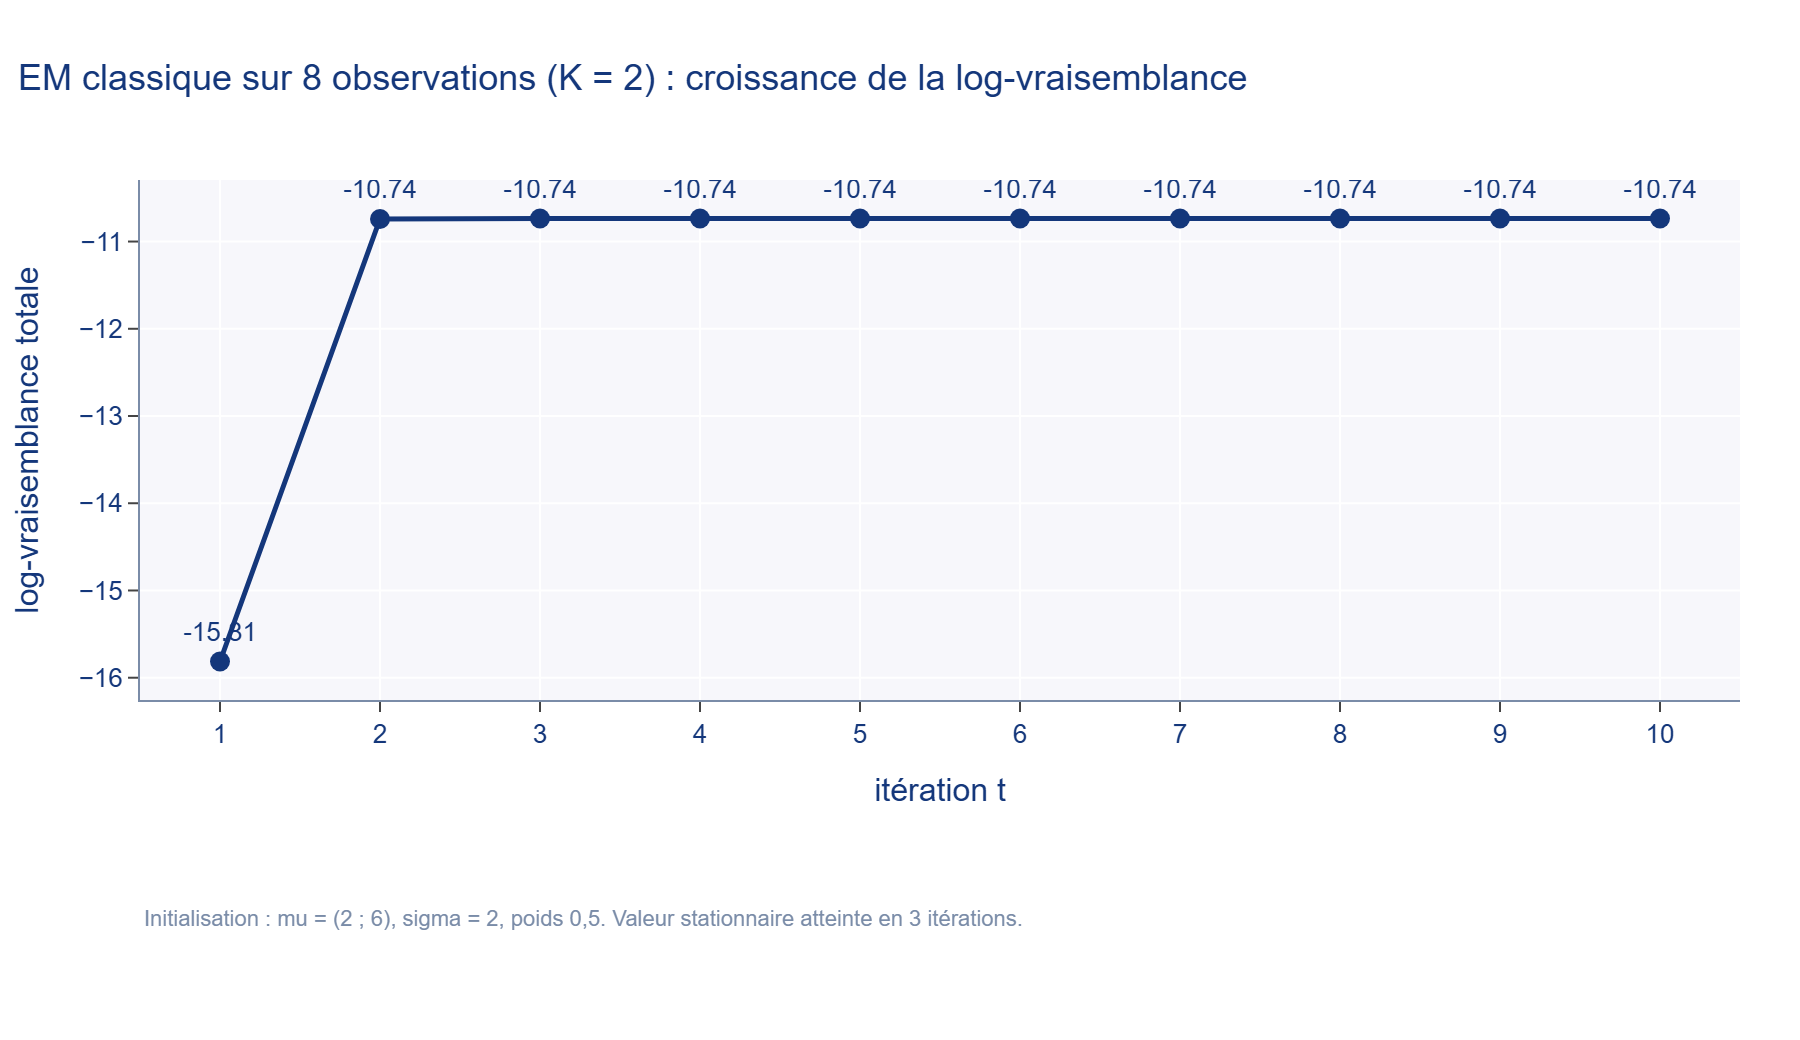
\includegraphics[width=0.85\textwidth]{figures/fig01.png}
\caption{Évolution de la log-vraisemblance au fil des itérations (exemple numérique de la section 1.6.4). La courbe est croissante puis stationnaire dès la troisième itération, ce qui illustre la garantie de monotonie établie à la section 1.6.2.f.}
\label{fig:1_1}
\end{figure}
\subsection{Variantes de l'EM classique}
\begin{table}[H]
\centering
\small
\setlength{\tabcolsep}{0.14cm}
\begin{tabular}{|p{3.54cm}|p{3.54cm}|p{3.54cm}|p{3.54cm}|}
\hline
\textbf{Variante} & \textbf{Modification} & \textbf{Avantage} & \textbf{Inconvénient} \\
\hline
EM standard & Aucune & Simple, convergence garantie & Lent sur grandes données \\
\hline
EM stochastique (SEM) & Étape E : tirage aléatoire & Évite certains optima locaux & Pas de monotonie \\
\hline
EM online & Mise à jour incrémentale & Scalable & Choix du taux d'apprentissage \\
\hline
EM généralisé (GEM) & Étape M approchée & Flexible & Convergence plus lente \\
\hline
EM accéléré (ECME) & Étape CM-E alternée & Convergence plus rapide & Complexité accrue \\
\hline
\end{tabular}
\caption{Principales variantes de l'algorithme EM classique}
\label{tab:1_3}
\end{table}
L'EM stochastique, proposé par Celeux et Diebolt (1985), modifie l'étape E en remplaçant le calcul des responsabilités par un tirage aléatoire : chaque observation est assignée à une seule composante selon la distribution définie par les responsabilités. Cette introduction de stochasticité permet d'éviter certains optima locaux, de calculer des estimations d'incertitude empiriques, et d'explorer plus largement l'espace des paramètres, au prix de la perte de la propriété de monotonie de la vraisemblance.

Pour les grandes bases de données, l'EM standard, dit « batch », traite l'ensemble des données à chaque itération, ce qui peut se révéler prohibitif. L'EM online, proposé par Sato et Ishii (2000) puis par Cappé et Moulines (2009), met à jour les paramètres après chaque observation ou mini-lot, réduisant drastiquement le coût par itération, et converge dans les mêmes conditions que l'EM standard sous des conditions de type Robbins-Monro sur le taux d'apprentissage.

L'EM généralisé remplace l'étape M exacte par une étape qui améliore, sans nécessairement maximiser, la fonction Q : on requiert seulement Q($\theta ^{t+1}$ | $\theta ^{t}$) $\geq $ Q($\theta ^{t}$ | $\theta ^{t}$), au lieu d'une maximisation exacte. La propriété de croissance monotone de la vraisemblance est préservée sous cette condition plus faible, ce qui rend le GEM utile lorsque l'étape M exacte est coûteuse ou n'admet pas de solution analytique.

Enfin, l'application originale ayant motivé l'article de Dempster et al. était précisément le traitement des données manquantes. Lorsque certaines composantes de $x_{i}$ sont manquantes, on peut traiter les valeurs manquantes comme des variables latentes supplémentaires, et l'algorithme EM impute naturellement ces valeurs en calculant leur espérance conditionnelle à l'étape E. Cette approche est asymptotiquement plus efficace que l'imputation simple et produit des estimateurs cohérents sous l'hypothèse MCAR ou MAR.

\subsection{Extension aux données séquentielles : l'algorithme de Baum-Welch}
Une application particulièrement importante de l'algorithme EM, mentionnée à plusieurs reprises dans ce mémoire (tableau 1.1, sections 1.6.1 et 3.1.3), concerne les modèles de Markov cachés (HMM), utilisés notamment en bio-informatique et en finance. Contrairement au GMM, où les observations sont supposées indépendantes conditionnellement à leur variable latente, un HMM suppose que la séquence des variables latentes ($z_{1}$, \ldots{}, z\_T) forme elle-même une chaîne de Markov : $z_{t}$ dépend de $z_{t-1}$ selon une matrice de transition A, et chaque observation $x_{t}$ dépend de l'état caché courant $z_{t}$ selon une matrice d'émission B. Cette structure séquentielle empêche le calcul direct des responsabilités comme à l'équation (1.15), puisque les variables latentes ne sont plus indépendantes entre elles : l'étape E doit être remplacée par l'algorithme forward-backward, qui exploite la structure de chaîne pour calculer efficacement, par programmation dynamique, les probabilités a posteriori nécessaires. L'algorithme résultant, connu sous le nom d'algorithme de Baum-Welch (Baum et al., 1970), est historiquement antérieur à la formalisation générale de Dempster, Laird et Rubin, mais en constitue, comme le notent ces derniers dans leur article de 1977, un cas particulier.

\textbf{Illustration numérique. }Considérons un HMM discret à deux états cachés (« Beau temps » = B, « Pluvieux » = P), avec une matrice de transition A = [[0,7 ; 0,3], [0,4 ; 0,6]] ($A_{ij}$ = P($z_{t+1}$=j | $z_{t}$=i)), et une matrice d'émission B qui associe à chaque état une probabilité d'observer « Parapluie » (Pa) ou « Pas de parapluie » (NPa) : B(B) = [0,1 ; 0,9] et B(P) = [0,8 ; 0,2]. Étant donné une courte séquence observée O = (NPa, Pa, Pa), l'étape E (forward-backward) calcule, pour chaque instant t et chaque état i, la probabilité a posteriori $\gamma _{t}$(i) = p($z_{t}$=i | O), de la même manière que $r_{ik}$ à l'équation (1.15) pour le GMM, mais en tenant compte de la dépendance séquentielle via les récursions forward $\alpha _{t}$(i) = [$\Sigma _{j}$ $\alpha _{t-1}$(j) $A_{ji}$] $B_{i}$($o_{t}$) et backward $\beta _{t}$(i) = $\Sigma _{j}$ $A_{ij}$ $B_{j}$($o_{t+1}$) $\beta _{t+1}$(j).

Une fois les quantités $\gamma _{t}$(i) calculées, l'étape M du Baum-Welch réestime les matrices A et B par des formules directement analogues à l'équation (1.16) du GMM, en remplaçant les responsabilités $r_{ik}$ par les quantités $\gamma _{t}$(i) et $\xi _{t}$(i,j) = p($z_{t}$=i, $z_{t+1}$=j | O) : Â$_{ij}$ = $\Sigma _{t}$ $\xi _{t}$(i,j) / $\Sigma _{t}$ $\gamma _{t}$(i), et $\hat{B}$$_{i}$(v) = $\Sigma $\_\{t : $o_{t}$=v\} $\gamma _{t}$(i) / $\Sigma _{t}$ $\gamma _{t}$(i). Cette correspondance formelle entre les mises à jour du Baum-Welch et celles du GMM illustre concrètement l'affirmation, faite à la section 1.6.1, selon laquelle l'EM constitue un cadre général unifiant des algorithmes historiquement développés de façon indépendante : le Baum-Welch n'est rien d'autre qu'un EM classique dans lequel l'étape E est rendue efficace, par programmation dynamique, pour tenir compte de la dépendance séquentielle entre variables latentes successives  une adaptation que l'on retrouve, sous une forme analogue, dans les extensions séquentielles de l'EM variationnel évoquées à la section 1.7.7.

\textbf{Calcul numérique complet de l'étape E. }Pour rendre entièrement concret le mécanisme décrit ci-dessus, calculons explicitement les quantités forward $\alpha _{t}$(i), backward $\beta _{t}$(i) et les probabilités a posteriori $\gamma _{t}$(i) pour la séquence observée O = (NPa, Pa, Pa), avec les matrices A et B et la distribution initiale $\pi _{0}$ = (0,6 ; 0,4) données ci-dessus. Le tableau 1.4 présente le détail de ce calcul.

\begin{table}[H]
\centering
\small
\setlength{\tabcolsep}{0.09cm}
\begin{tabular}{|p{1.71cm}|p{1.71cm}|p{1.71cm}|p{1.71cm}|p{1.71cm}|p{1.71cm}|p{1.71cm}|p{1.71cm}|}
\hline
\textbf{t} & \textbf{Observation $o_{t}$} & \textbf{$\alpha _{t}$(B)} & \textbf{$\alpha _{t}$(P)} & \textbf{$\beta _{t}$(B)} & \textbf{$\beta _{t}$(P)} & \textbf{$\gamma _{t}$(B)} & \textbf{$\gamma _{t}$(P)} \\
\hline
1 & NPa & 0,540 & 0,080 & 0,147 & 0,262 & 0,791 & 0,210 \\
\hline
2 & Pa & 0,041 & 0,168 & 0,310 & 0,520 & 0,127 & 0,873 \\
\hline
3 & Pa & 0,010 & 0,091 & 1,000 & 1,000 & 0,096 & 0,904 \\
\hline
\end{tabular}
\caption{Calcul détaillé des quantités forward, backward et a posteriori pour O = (NPa, Pa, Pa)}
\label{tab:1_4}
\end{table}
La dernière colonne du tableau se lit comme suit : après observation de la séquence complète (NPa, Pa, Pa), la probabilité a posteriori que le temps ait été « Beau » (B) au premier instant est de 0,791 (malgré l'absence de parapluie ce jour-là, cohérent avec un temps beau), tandis qu'elle chute à 0,127 au deuxième instant et à 0,096 au troisième, la présence du parapluie aux instants 2 et 3 rendant l'état « Pluvieux » (P) très majoritairement probable a posteriori ($\gamma _{2}$(P) = 0,873 et $\gamma _{3}$(P) = 0,904). On notera que $\Sigma _{i}$ $\gamma _{t}$(i) = 1 à chaque instant t, exactement comme $\Sigma _{k}$ $r_{ik}$ = 1 pour les responsabilités du GMM à l'équation (1.15)  les quantités $\gamma _{t}$(i) jouant, pour le HMM, exactement le rôle que jouent les responsabilités $r_{ik}$ pour le GMM. La probabilité totale de la séquence observée, obtenue en sommant $\alpha _{t}$(i) sur i au dernier instant, vaut p(O | A, B, $\pi _{0}$) = $\alpha _{3}$(B) + $\alpha _{3}$(P) = 0,010 + 0,091 = 0,100.

\subsection{Avantages de l'EM classique}
\begin{itemize}
\item \textbf{Simplicité et transparence : }l'algorithme EM est conceptuellement clair et facile à comprendre. Les deux étapes E et M ont des interprétations directes, et les mises à jour sont souvent analytiques, ce qui facilite l'implémentation, le débogage et l'adaptation à de nouveaux modèles.
\item \textbf{Garantie de convergence monotone : }la log-vraisemblance ne peut que croître ou rester constante à chaque itération. Cette propriété offre une sécurité précieuse : l'algorithme ne peut pas « se dégrader » au fil des itérations, et la log-vraisemblance constitue un critère de convergence naturel.
\item \textbf{Efficacité computationnelle par itération : }chaque itération de l'EM a un coût fixe en O($NKD^{2}$), aisément vectorisable. Pour des problèmes de taille modérée, l'EM est extrêmement rapide et se parallélise bien.
\item \textbf{Applicabilité universelle : }l'EM s'applique à n'importe quel modèle probabiliste pour lequel p(Z | X, $\theta $) est calculable et $\mathbb{E}$[log p(X, Z | $\theta $)] est maximisable, ce qui couvre une immense variété de modèles en pratique.
\item \textbf{Gestion naturelle des données incomplètes : }par construction, l'EM intègre sur les valeurs manquantes, produisant des estimateurs asymptotiquement efficaces sans recourir à des heuristiques d'imputation.
\item \textbf{Convergence rapide loin de l'optimum : }bien que la convergence soit linéaire asymptotiquement, l'EM converge souvent très rapidement lors des premières itérations, permettant d'obtenir de bonnes solutions en peu d'itérations.
\end{itemize}
\subsection{Inconvénients et limites de l'EM classique}
\begin{itemize}
\item \textbf{Convergence vers des optima locaux : }l'EM converge vers un point stationnaire de la vraisemblance, généralement un maximum local. Sur les problèmes multimodaux, comme les GMM à composantes proches, la solution trouvée peut être significativement sous-optimale par rapport au maximum global.
\item \textbf{Nécessité de spécifier K a priori : }le nombre de composantes K doit être fixé avant l'exécution de l'algorithme. Une mauvaise spécification de K conduit inévitablement à des résultats sous-optimaux : la sous-estimation entraîne des composantes trop larges fusionnant des groupes distincts, tandis que la surestimation entraîne des composantes redondantes ou dégénérées. C'est précisément cette limite que nous illustrerons expérimentalement au chapitre 2, à travers un cas où K est volontairement surestimé.
\item \textbf{Absence de quantification de l'incertitude : }l'EM classique fournit des estimations ponctuelles $\hat{\theta }$, sans aucune distribution autour de ces estimations, ce qui pose problème dans de nombreuses applications, en médecine ou en finance notamment, où l'incertitude sur les paramètres est aussi importante que les paramètres eux-mêmes pour la prise de décision.
\item \textbf{Singularités et dégénérescences : }un problème bien connu du GMM est la possibilité de convergence vers des solutions singulières, une composante pouvant s'effondrer sur un seul point de données, sa variance tendant vers zéro, ce qui provoque une divergence de la log-vraisemblance vers l'infini. Des stratégies ad hoc, telles que la régularisation de la covariance, sont nécessaires pour éviter ce problème.
\item \textbf{Lenteur de convergence : }le taux de convergence linéaire peut rendre l'algorithme très lent dans les régions proches de l'optimum, en particulier lorsque les composantes se chevauchent fortement.
\item \textbf{Scalabilité limitée : }la version batch standard nécessite de traiter toutes les données à chaque itération, ce qui devient prohibitif pour des bases de plusieurs millions d'observations, sans recourir aux variantes online ou mini-batch.
\end{itemize}
\section{L'algorithme EM variationnel}
\subsection{Motivation et cadre général}
Les limitations identifiées à la section 1.6.8 motivent naturellement le développement d'une approche plus riche. L'EM variationnel émerge à la confluence de deux courants : l'inférence bayésienne, qui traite les paramètres comme des variables aléatoires et vise à caractériser leur distribution a posteriori complète, et l'optimisation variationnelle, qui transforme le problème d'inférence  généralement intractable  en un problème d'optimisation sur un espace de distributions plus simples.

Le cadre variationnel trouve ses racines dans les travaux de Hinton et van Camp (1993) sur les réseaux de neurones bayésiens, de Peterson et Anderson (1987) sur les champs moyens pour les réseaux de Boltzmann, et a été synthétisé et généralisé par Jordan, Ghahramani, Jaakkola et Saul (1999) dans leur article fondateur sur les méthodes variationnelles pour les modèles graphiques. Depuis lors, l'inférence variationnelle est devenue l'une des méthodes d'inférence approchée les plus utilisées en apprentissage automatique probabiliste. Pour le mélange gaussien, l'application aux priors conjugués suit Attias (2000), Corduneanu et Bishop (2001) et Bishop (2006, chapitre 10).

\subsection{Inférence variationnelle}
\subsubsection{a) Le problème d'inférence bayésienne}
Dans le cadre bayésien complet, on cherche à calculer la distribution a posteriori jointe sur les paramètres et les variables latentes, p($\theta $, Z | X) = p(X | Z, $\theta $) p(Z | $\theta $) p($\theta $) / p(X). Le dénominateur, p(X) = $\int \int $ p(X | Z, $\theta $) p(Z | $\theta $) p($\theta $) dZ $d\theta $, est la vraisemblance marginale, ou évidence. Son calcul nécessite une intégrale de haute dimension, généralement intractable analytiquement pour des modèles non triviaux. Sans ce dénominateur, on ne peut pas normaliser la distribution a posteriori. L'inférence variationnelle contourne ce problème en remplaçant le calcul exact de p($\theta $, Z | X) par l'optimisation d'une approximation.

\subsubsection{b) La famille variationnelle et le problème d'optimisation}
L'inférence variationnelle introduit une famille de distributions $\mathcal{Q}$ = \{q($\theta $, Z | $\lambda $), $\lambda $ $\in $ $\Lambda $\}, paramétrée par des paramètres variationnels $\lambda $. L'objectif est de trouver le membre de cette famille le plus proche de la vraie distribution a posteriori, au sens de la divergence de Kullback-Leibler :

\begin{equation}
\begin{adjustbox}{max width=0.92\linewidth}$\displaystyle q*(\theta {,} Z) = \operatorname*{argmin}_{q \in  \mathcal{Q}} KL[q(\theta {,} Z) \Vert  p(\theta {,} Z | X)]$\end{adjustbox}
\tag{1.20}
\label{eq:1_20}
\end{equation}
Cette divergence ne peut pas être calculée directement, car elle fait intervenir p(X) dans sa normalisation. On montre cependant que minimiser cette divergence est équivalent à maximiser l'ELBO, qui lui est calculable :

\begin{equation}
\begin{adjustbox}{max width=0.92\linewidth}$\displaystyle ELBO(q) = \mathbb{E}_{q}[\log  p(X{,} Z{,} \theta )] - \mathbb{E}_{q}[\log  q(\theta {,} Z)]$\end{adjustbox}
\tag{1.21}
\label{eq:1_21}
\end{equation}
Cette reformulation est la clé de l'inférence variationnelle : un problème d'inférence, à savoir le calcul d'une distribution, est transformé en un problème d'optimisation, à savoir la maximisation d'une fonctionnelle de q, qui peut être traité par des algorithmes d'optimisation standard.

\subsubsection{c) L'ELBO comme objectif d'apprentissage}
L'ELBO peut être décomposé de deux manières complémentaires, chacune offrant une interprétation différente. La première décomposition montre l'ELBO comme la différence entre la vraisemblance attendue et la complexité du modèle :

\begin{equation}
\begin{adjustbox}{max width=0.92\linewidth}$\displaystyle ELBO(q) = \mathbb{E}_{q}[\log  p(X | Z{,} \theta )] - KL[q(\theta {,} Z) \Vert  p(\theta {,} Z)]$\end{adjustbox}
\tag{1.22}
\label{eq:1_22}
\end{equation}
Le premier terme, la log-vraisemblance attendue sous q, mesure la qualité de l'ajustement aux données ; le second terme, la divergence KL entre la distribution variationnelle et le prior joint, pénalise les distributions q qui s'écartent trop du prior, réalisant ainsi une forme de régularisation bayésienne automatique. La maximisation de l'ELBO réalise donc un compromis naturel entre ajustement aux données et fidélité au prior.

La seconde décomposition, déjà introduite à la section 1.5.3, montre l'ELBO comme une borne inférieure de la log-évidence : log p(X) = ELBO(q) + KL[q($\theta $, Z) $\Vert $ p($\theta $, Z | X)] $\geq $ ELBO(q). Cette décomposition est fondamentale pour la sélection de modèle bayésien : un modèle dont l'ELBO est plus élevé à la convergence est préférable, car son évidence est plus grande, ce qui implique qu'il explique mieux les données tout en contrôlant la complexité.

\subsection{Formulation de l'EM variationnel}
\subsubsection{a) L'hypothèse du champ moyen}
L'hypothèse la plus courante pour définir la famille variationnelle $\mathcal{Q}$ est l'hypothèse du champ moyen, qui suppose une factorisation complète de la distribution variationnelle sur les différentes variables :

\begin{equation}
\begin{adjustbox}{max width=0.92\linewidth}$\displaystyle q(\theta {,} Z) = q(\theta ) \prod _{i} q(z_{i}) = q(\pi ) \prod _{k} q(\mu _{k}{,} \Lambda _{k}) \prod _{i} q(z_{i})$\end{adjustbox}
\tag{1.23}
\label{eq:1_23}
\end{equation}
Cette hypothèse ignore les corrélations a posteriori entre les paramètres $\theta $ et les variables latentes Z, ainsi qu'entre les variables latentes de différentes observations. Si cette indépendance est rarement exacte dans la vraie distribution a posteriori, elle simplifie considérablement le problème d'optimisation en le rendant décomposable en sous-problèmes indépendants, tout en restant une approximation raisonnable dans de nombreuses applications.

\subsubsection{b) Les mises à jour variationnelles optimales}
Sous l'hypothèse du champ moyen, la solution variationnelle optimale pour chaque facteur $q_{j}$($z_{j}$) est donnée par la formule du champ moyen variationnel :

\begin{equation}
\begin{adjustbox}{max width=0.92\linewidth}$\displaystyle \log  q*_{j}(z_{j}) = \mathbb{E}_{q(z \setminus z_{j})}[\log  p(X{,} Z{,} \theta )] + constante$\end{adjustbox}
\tag{1.24}
\label{eq:1_24}
\end{equation}
Cette mise à jour prend l'espérance de la log-distribution jointe par rapport à tous les autres facteurs, en maintenant $z_{j}$ fixe, la constante additive assurant la normalisation. Cette formule est générale et s'applique à n'importe quel facteur, qu'il s'agisse d'une variable latente ou d'un paramètre. Dans le cas des modèles conjugués, cette espérance peut être calculée analytiquement et conduit à une distribution de la même famille que le prior correspondant.

\subsubsection{c) Dérivation détaillée pour le mélange gaussien bayésien}
Cette section applique explicitement la formule générale du champ moyen variationnel, énoncée ci-dessus, au cas particulier du mélange gaussien bayésien, afin de montrer comment les formes de Dirichlet et de Normal-Wishart, utilisées dans l'algorithme de la section 1.7.3.d, se déduisent directement de cette formule générale plutôt que d'être postulées arbitrairement.

\textbf{Facteur q($\pi $). }En isolant, dans le logarithme de la distribution jointe complète log p(X, Z, $\pi $, $\mu $, $\Lambda $), les seuls termes qui dépendent de $\pi $, on obtient log p(Z | $\pi $) + log p($\pi $) = $\Sigma _{i}$ $\Sigma _{k}$ $z_{ik}$ log $\pi _{k}$ + $\Sigma _{k}$ ($\alpha _{0}$-1) log $\pi _{k}$ + constante, où $z_{ik}$ désigne l'indicatrice $z_{i}$ = k. En appliquant la formule du champ moyen, on prend l'espérance de cette expression par rapport à q(Z), ce qui revient à remplacer $z_{ik}$ par son espérance $r_{ik}$ = $\mathbb{E}$\_q[$z_{ik}$] :

\begin{equation}
\begin{adjustbox}{max width=0.92\linewidth}$\displaystyle \log  q*(\pi ) = \Sigma _{k} (\alpha _{0} - 1 + N_{k}) \log  \pi _{k} + constante{,}  où N_{k} = \Sigma _{i} r_{ik}$\end{adjustbox}
\tag{1.25}
\label{eq:1_25}
\end{equation}
Cette expression est, à une constante de normalisation près, exactement le logarithme de la densité d'une distribution de Dirichlet de paramètres $\alpha _{k}$ = $\alpha _{0}$ + $N_{k}$. On retrouve ainsi directement, par simple application de la formule générale, la mise à jour $\alpha _{k}$ = $\alpha _{0}$ + $N_{k}$ utilisée à la section 1.7.3.d, sans qu'il soit nécessaire de la postuler : elle découle mécaniquement de la conjugaison entre le prior de Dirichlet et la vraisemblance catégorielle.

\textbf{Facteur q($\mu _{k}$, $\Lambda _{k}$). }De façon similaire, en isolant les termes qui dépendent de ($\mu _{k}$, $\Lambda _{k}$) dans log p(X, Z, $\pi $, $\mu $, $\Lambda $), on obtient une contribution de la vraisemblance gaussienne, $\Sigma _{i}$ $r_{ik}$ log $\mathcal{N}$($x_{i}$ | $\mu _{k}$, $\Lambda _{k}^{-1}$), à laquelle s'ajoute le logarithme du prior Normal-Wishart log p($\mu _{k}$, $\Lambda _{k}$). Cette somme, une fois réorganisée en complétant le carré sur $\mu _{k}$  une manipulation algébrique standard pour les formes quadratiques gaussiennes , se réécrit comme le logarithme d'une densité Normal-Wishart de paramètres mis à jour :

\begin{equation}
\begin{adjustbox}{max width=0.92\linewidth}$\displaystyle \beta _{k} = \beta _{0} + N_{k}{,}   m_{k} = (\beta _{0}m_{0} + N_{k}\bar{x}_{k})/\beta _{k}{,}   \nu _{k} = \nu _{0} + N_{k}{,}   W_{k}^{-1} = W_{0}^{-1} + N_{k}S_{k} + [\beta _{0}N_{k}/(\beta _{0}+N_{k})](\bar{x}_{k}-m_{0})(\bar{x}_{k}-m_{0})^{T}$\end{adjustbox}
\tag{1.26}
\label{eq:1_26}
\end{equation}
où $\bar{x}$$_{k}$ et $S_{k}$ désignent respectivement la moyenne et la covariance empiriques pondérées par les responsabilités, telles que définies à la section 1.7.3.d. Le terme $\beta _{k}$ s'interprète comme une « taille d'échantillon effective augmentée » (la taille d'échantillon effective $N_{k}$ à laquelle s'ajoute la pseudo-taille d'échantillon $\beta _{0}$ du prior), tandis que le dernier terme correctif dans la mise à jour de $W_{k}^{-1}$ traduit l'incertitude supplémentaire due à l'écart entre la moyenne empirique du cluster $\bar{x}$$_{k}$ et la moyenne a priori $m_{0}$ : plus cet écart est grand par rapport à la confiance relative accordée au prior (mesurée par le rapport $\beta _{0}N_{k}$/($\beta _{0}$+$N_{k}$)), plus la matrice de précision $W_{k}^{-1}$ voit sa valeur augmenter, ce qui élargit d'autant la distribution a posteriori sur $\mu _{k}$.

Cette dérivation confirme, de façon rigoureuse, que les formules de mise à jour utilisées à la section 1.7.3.d ne sont pas de simples analogues heuristiques de l'étape M classique : elles sont la conséquence mathématique directe et nécessaire de l'application de la formule générale du champ moyen variationnel au choix spécifique de priors conjugués effectué à la section 1.4.2. Ce même schéma de dérivation  isoler les termes pertinents dans la log-distribution jointe, prendre leur espérance sous les autres facteurs, puis reconnaître la forme conjuguée résultante  se généralise sans difficulté conceptuelle à tout modèle à variables latentes construit à partir de distributions conjuguées, ce qui explique la popularité de l'hypothèse du champ moyen dans la pratique de l'inférence variationnelle.

\subsubsection{d) L'algorithme EM variationnel}
L'algorithme EM variationnel alterne entre deux étapes, analogues aux étapes E et M de l'EM classique, mais opérant sur des distributions plutôt que sur des estimations ponctuelles. L'algorithme prend en entrée les observations X, un nombre maximal de composantes Kmax, les hyperparamètres du prior \{$\alpha _{0}$, $m_{0}$, $\beta _{0}$, $W_{0}$, $\nu _{0}$\}, ainsi qu'un critère d'arrêt $\varepsilon $.

\textbf{Initialisation. }Les paramètres variationnels sont initialisés : $\alpha _{k}$ = $\alpha _{0}$ + N/K, $N_{k}$ = N/K, $m_{k}$ = $m_{0}$ + perturbation aléatoire, $\beta _{k}$ = $\beta _{0}$ + $N_{k}$, $\nu _{k}$ = $\nu _{0}$ + $N_{k}$, $W_{k}$ = $W_{0}$.

\textbf{Étape E variationnelle. }Pour chaque observation i et chaque composante k, on calcule :

\begin{equation}
\begin{adjustbox}{max width=0.92\linewidth}$\displaystyle \log  \rho _{ik} = \mathbb{E}[\log  \pi _{k}] + \tfrac{1}{2} \mathbb{E}[\log |\Lambda _{k}|] - (D/2) \log (2\pi ) - \tfrac{1}{2} \mathbb{E}[(x_{i}-\mu _{k})^{T}\Lambda _{k}(x_{i}-\mu _{k})]$\end{adjustbox}
\tag{1.27}
\label{eq:1_27}
\end{equation}
puis on normalise pour obtenir les responsabilités : $r_{ik}$ = exp(log $\rho _{ik}$) / $\Sigma _{j}$ exp(log $\rho _{ij}$).

\textbf{Étape M variationnelle. }Pour chaque composante k, on calcule $N_{k}$ = $\Sigma _{i}$ $r_{ik}$, $\bar{x}$$_{k}$ = (1/$N_{k}$) $\Sigma _{i}$ $r_{ik}$ $x_{i}$, et $S_{k}$ = (1/$N_{k}$) $\Sigma _{i}$ $r_{ik}$ ($x_{i}$-$\bar{x}$$_{k}$)($x_{i}$-$\bar{x}$$_{k}$)$^{T}$, avant de mettre à jour les paramètres des lois de Dirichlet et Normal-Wishart :

\begin{equation}
\begin{adjustbox}{max width=0.92\linewidth}$\displaystyle \alpha _{k} = \alpha _{0} + N_{k}{,}  \beta _{k} = \beta _{0} + N_{k}{,}  m_{k} = (\beta _{0}m_{0} + N_{k}\bar{x}_{k})/\beta _{k}{,}  \nu _{k} = \nu _{0} + N_{k}$\end{adjustbox}
\tag{1.28}
\label{eq:1_28}
\end{equation}
ainsi que la mise à jour de la matrice d'échelle $W_{k}^{-1}$ = $W_{0}^{-1}$ + $N_{k}S_{k}$ + [$\beta _{0}N_{k}$/($\beta _{0}$+$N_{k}$)] ($\bar{x}$$_{k}$-$m_{0}$)($\bar{x}$$_{k}$-$m_{0}$)$^{T}$. L'ELBO est ensuite calculé, et les composantes telles que $\alpha _{k}$ $\approx $ $\alpha _{0}$ sont élaguées, selon le mécanisme détaillé à la section 1.7.4. Ces deux étapes sont répétées jusqu'à convergence de l'ELBO, l'algorithme retournant alors la distribution q*($\theta $) ainsi que le nombre effectif de composantes actives, K\_effectif.

\subsubsection{e) Calcul des espérances nécessaires}
L'étape E variationnelle requiert le calcul de plusieurs espérances par rapport aux distributions variationnelles courantes, espérances qui admettent des formes analytiques pour les distributions conjuguées utilisées. Pour la distribution de Dirichlet q($\pi $) = Dir($\alpha _{1}$, \ldots{}, $\alpha K$), l'espérance du logarithme du poids est donnée par :

\begin{equation}
\begin{adjustbox}{max width=0.92\linewidth}$\displaystyle \mathbb{E}[\log  \pi _{k}] = \psi (\alpha _{k}) - \psi (\Sigma _{j} \alpha _{j})$\end{adjustbox}
\tag{1.29}
\label{eq:1_29}
\end{equation}
où $\psi $ désigne la fonction digamma. Pour la distribution de Wishart q($\Lambda _{k}$) = $\mathcal{W}$($W_{k}$, $\nu _{k}$), on obtient $\mathbb{E}$[log|$\Lambda _{k}$|] = $\Sigma _{j=1}^{D}$ $\psi $[($\nu _{k}$+1-j)/2] + D log 2 + log|$W_{k}$|. Enfin, pour la distribution normale q($\mu _{k}$|$\Lambda _{k}$) = $\mathcal{N}$($m_{k}$, ($\beta _{k}\Lambda _{k}$)$^{-1}$), l'espérance de la forme quadratique vaut :

\begin{equation}
\begin{adjustbox}{max width=0.92\linewidth}$\displaystyle \mathbb{E}[(x-\mu _{k})^{T}\Lambda _{k}(x-\mu _{k})] = D/\beta _{k} + \nu _{k}(x-m_{k})^{T}W_{k}(x-m_{k})$\end{adjustbox}
\tag{1.30}
\label{eq:1_30}
\end{equation}
\subsection{Sélection automatique du nombre de composantes}
L'une des propriétés les plus remarquables et pratiquement importantes de l'EM variationnel est sa capacité à déterminer automatiquement le nombre effectif de composantes dans un mélange gaussien bayésien. Ce mécanisme, qui constitue l'un des apports majeurs de l'EM variationnel par rapport à l'EM classique, mérite une explication détaillée, car il sera au cœur de l'étude expérimentale présentée au chapitre 2.

La clé de ce mécanisme réside dans le prior de Dirichlet Dir($\alpha _{0}$, \ldots{}, $\alpha _{0}$) placé sur les poids de mélange. Lorsque $\alpha _{0}$ est petit  typiquement $\alpha _{0}$ = 1/Kmax ou $\alpha _{0}$ = 10$^{-3}$ , ce prior favorise fortement les solutions parcimonieuses, où la plupart des poids sont proches de zéro, c'est-à-dire les solutions n'utilisant qu'un petit nombre de composantes actives.

Lors de l'optimisation variationnelle, une composante k pour laquelle les données ne fournissent pas de support suffisant voit son paramètre $\alpha _{k}$ rester proche de $\alpha _{0}$, faute d'augmentation significative lors de l'étape M. Cela se traduit par $\mathbb{E}$[log $\pi _{k}$] proche d'une constante fortement négative à l'étape E, ce qui rend les responsabilités $r_{ik}$ proches de zéro pour toutes les observations : la composante est alors effectivement « éteinte » et n'influence plus le modèle. En pratique, on considère qu'une composante est inactive lorsque $N_{k}$ = $\Sigma _{i}$ $r_{ik}$ < 1.

Ce mécanisme d'élagage automatique constitue une forme de rasoir d'Occam bayésien : le modèle utilise spontanément le nombre minimal de composantes nécessaires pour expliquer les données, sans sur-ajustement. En initialisant avec un Kmax suffisamment grand  par exemple Kmax = 20 pour un problème où l'on attend entre 3 et 5 groupes , l'algorithme converge naturellement vers une solution utilisant uniquement le nombre approprié de composantes actives, sans qu'il soit nécessaire d'exécuter l'algorithme séparément pour chaque valeur candidate de K, comme l'exigerait l'EM classique.

\subsection{Exemple numérique illustratif}
Afin de rendre plus concret le mécanisme d'élagage décrit ci-dessus, reprenons l'exemple numérique de la section 1.6.4 : les huit observations scalaires X = \{0,5 ; 1,0 ; 1,2 ; 1,8 ; 7,1 ; 7,5 ; 8,0 ; 8,3\}, qui forment visiblement deux groupes bien séparés. Appliquons cette fois l'EM variationnel avec Kmax = 3 composantes  soit une de plus que le nombre réel de groupes , un prior de Dirichlet de concentration $\alpha _{0}$ = 1/3, et des priors Normal-Wishart non informatifs ($\beta _{0}$ = 10$^{-3}$, $\nu _{0}$ = 1, $W_{0}$ = 1).

L'algorithme converge en 5 à 15 itérations selon l'initialisation (critère $|\Delta \mathrm{ELBO}| < 10^{-6}$), vers la même solution dans les dix essais réalisés (graines 0 à 4, initialisation par les hyperparamètres ou par k-means). Le tableau 1.5 présente les paramètres finaux obtenus pour chacune des trois composantes.

\begin{table}[H]
\centering
\small
\setlength{\tabcolsep}{0.14cm}
\begin{tabular}{|p{2.77cm}|p{2.77cm}|p{2.77cm}|p{2.77cm}|p{2.77cm}|}
\hline
\textbf{Composante k} & \textbf{$\alpha _{k}$} & \textbf{Poids $\pi _{k}$ = $\alpha _{k}$/$\Sigma \alpha $} & \textbf{Moyenne $m_{k}$} & \textbf{Interprétation} \\
\hline
1 & 4,333 & 0,482 & 7,724 & Groupe des grandes valeurs (actif) \\
\hline
2 & 4,333 & 0,482 & 1,126 & Groupe des petites valeurs (actif) \\
\hline
3 & 0,333 & 0,037 & 4,425 & Composante élaguée ($\alpha _{k}$ = $\alpha _{0}$) \\
\hline
\end{tabular}
\caption{Résultat de l'EM variationnel sur l'exemple numérique à 8 observations (Kmax = 3)}
\label{tab:1_5}
\end{table}
Ce résultat illustre de façon particulièrement nette le mécanisme théorique décrit ci-dessus. Les deux premières composantes se partagent presque également la masse de probabilité (poids 0,482 chacune), avec des moyennes de 7,724 et 1,126 qui coïncident, à $10^{-3}$ près, avec les moyennes empiriques des deux groupes et avec la solution de l'EM classique de la section 1.6.4 (7,725 et 1,125). La troisième composante, en revanche, voit son paramètre $\alpha _{k}$ rester exactement égal à sa valeur initiale $\alpha _{0}$ = 1/3 = 0,333, signe que $N_{k}$ = $\alpha _{k}$ - $\alpha _{0}$ = 0 : aucune observation, même partiellement, ne lui a été attribuée au cours de la convergence. Cette composante est donc entièrement inactive, et le modèle retient effectivement K\_effectif = 2 composantes actives, exactement le nombre réel de groupes  un résultat que l'EM classique, avec K fixé à l'avance, ne peut pas produire de lui-même : il faudrait, pour l'EM classique, comparer explicitement les solutions à K = 2 et K = 3 au moyen d'un critère externe tel que le BIC, alors que l'EM variationnel effectue cette sélection de façon endogène, en une seule exécution.

\subsection{Calcul de l'ELBO et critère de convergence}
Pour le mélange gaussien bayésien sous l'hypothèse du champ moyen, l'ELBO peut être calculé analytiquement à chaque itération. Il se décompose sous la forme :

\begin{equation}
\begin{adjustbox}{max width=0.92\linewidth}$\displaystyle ELBO = \mathbb{E}_{q}[\log  p(X|Z{,}\theta )] + \mathbb{E}_{q}[\log  p(Z|\pi )] + \mathbb{E}_{q}[\log  p(\pi )] + \Sigma _{k} \mathbb{E}_{q}[\log  p(\mu _{k}{,}\Lambda _{k})] - \mathbb{E}_{q}[\log  q(Z)] - \mathbb{E}_{q}[\log  q(\pi )] - \Sigma _{k} \mathbb{E}_{q}[\log  q(\mu _{k}{,}\Lambda _{k})]$\end{adjustbox}
\tag{1.31}
\label{eq:1_31}
\end{equation}
Chacun de ces termes peut être calculé analytiquement grâce aux formes conjuguées des distributions considérées ; leur expression complète est donnée par Bishop (2006, éq. 10.71 à 10.77) et implémentée à l'annexe B. L'ELBO constitue le critère de convergence naturel de l'EM variationnel : on arrête l'algorithme lorsque |ELBO(t) - ELBO(t-1)| < $\varepsilon $. Contrairement à l'EM classique, où la log-vraisemblance peut diverger vers l'infini en présence de singularités, l'ELBO de l'EM variationnel reste toujours borné, grâce à la régularisation bayésienne induite par les priors.

\subsection{Variantes avancées de l'EM variationnel}
\textbf{Inférence variationnelle naturelle. }L'inférence variationnelle standard utilise le gradient ordinaire de l'ELBO pour optimiser les paramètres variationnels. Une variante plus efficace utilise le gradient naturel, qui prend en compte la géométrie de l'espace des distributions à travers la métrique de Fisher. Les mises à jour par gradient naturel sont invariantes aux reparamétrisations et convergent généralement beaucoup plus rapidement que les mises à jour utilisant le gradient ordinaire.

\textbf{Inférence variationnelle stochastique (SVI). }Proposée par Hoffman et al. (2013), la SVI étend l'EM variationnel aux très grandes bases de données en utilisant des mini-lots. À chaque itération, les mises à jour variationnelles sont calculées sur un sous-ensemble des données avant de mettre à jour les paramètres globaux à l'aide d'un taux d'apprentissage décroissant. La SVI constitue l'analogue de l'EM online pour l'EM variationnel et a permis l'application de modèles bayésiens complexes à des corpus contenant plusieurs millions de documents.

\textbf{Inférence variationnelle amortie (VAE). }Les auto-encodeurs variationnels, introduits par Kingma et Welling (2014), représentent une généralisation profonde de l'EM variationnel aux modèles génératifs profonds. Le principe consiste à apprendre une fonction d'encodage q(Z|X, $\phi $), paramétrée par un réseau de neurones, qui approxime directement la distribution a posteriori. Cette stratégie, appelée amortisation de l'inférence, permet de traiter efficacement de nouvelles observations sans réoptimiser les paramètres variationnels pour chacune d'elles. Aujourd'hui, le VAE constitue l'un des modèles génératifs les plus influents en apprentissage profond.

\textbf{Normalizing Flows. }Une limitation importante de l'hypothèse du champ moyen est qu'elle restreint les distributions variationnelles à des familles factorisées souvent trop simples pour représenter fidèlement les corrélations de la distribution a posteriori. Les Normalizing Flows, proposés par Rezende et Mohamed (2015), permettent de construire des familles variationnelles beaucoup plus expressives en composant des transformations bijectives inversibles, tout en conservant la différentiabilité. Cette approche combine ainsi la flexibilité des modèles génératifs profonds avec la rigueur du cadre variationnel bayésien.

\subsection{Avantages de l'EM variationnel}
\begin{itemize}
\item \textbf{Quantification complète de l'incertitude : }l'EM variationnel fournit une distribution q*($\theta $) sur les paramètres, permettant de calculer des intervalles de crédibilité, des quantiles, et d'intégrer l'incertitude paramétrique dans les prédictions, propriété fondamentale dans les applications où la décision doit tenir compte de l'incertitude.
\item \textbf{Sélection automatique du nombre de composantes : }le mécanisme d'élagage variationnel détermine automatiquement le nombre effectif de composantes, éliminant la nécessité d'une sélection externe de K et permettant une inférence en une seule exécution plutôt qu'une série d'exécutions pour différentes valeurs de K.
\item \textbf{Régularisation bayésienne et robustesse : }l'intégration des distributions a priori protège naturellement contre le surapprentissage et les singularités, la divergence de Kullback-Leibler vers le prior dans l'ELBO agissant comme une régularisation qui empêche les composantes de s'effondrer sur des observations individuelles.
\item \textbf{ELBO comme critère de convergence et de sélection : }l'ELBO constitue une borne inférieure de la log-évidence et représente un critère de convergence naturel, informatif et comparable entre différents modèles, ce qui fournit un critère de sélection bayésien intégré.
\item \textbf{Cadre extensible aux modèles complexes : }le cadre variationnel s'étend naturellement aux modèles hiérarchiques complexes, aux modèles génératifs profonds tels que les VAE, ainsi qu'aux modèles comportant plusieurs niveaux de variables latentes, là où l'EM classique devient difficilement applicable.
\item \textbf{Convergence monotone de l'ELBO : }comme l'EM classique, l'EM variationnel garantit que l'ELBO ne décroît jamais entre deux itérations, propriété qui assure une grande stabilité numérique et facilite le diagnostic de la convergence.
\end{itemize}
\subsection{Inconvénients et limites de l'EM variationnel}
\begin{itemize}
\item \textbf{Biais d'approximation systématique : }l'hypothèse du champ moyen introduit un biais systématique dans l'approximation. La distribution variationnelle optimale q* tend généralement à sous-estimer la variance de la véritable distribution a posteriori, phénomène de zero-forcing lié à la divergence KL. Lorsque la distribution a posteriori est fortement multimodale ou présente de fortes corrélations, cette approximation peut devenir relativement grossière.
\item \textbf{Complexité d'implémentation : }la dérivation des mises à jour variationnelles pour un nouveau modèle nécessite une bonne maîtrise du calcul variationnel bayésien ainsi que de la famille exponentielle. L'implémentation correcte du calcul de l'ELBO pour le suivi de la convergence est sensiblement plus complexe que celle de l'EM classique.
\item \textbf{Sensibilité aux distributions a priori : }le choix des hyperparamètres des distributions a priori ($\alpha _{0}$, $m_{0}$, $\beta _{0}$, $W_{0}$, $\nu _{0}$) peut influencer de manière significative les résultats, particulièrement lorsque le nombre de données disponibles est limité, ce qui nécessite une expertise ou une procédure de calibration empirique.
\item \textbf{Convergence vers des optima locaux de l'ELBO : }la maximisation de l'ELBO reste susceptible de converger vers des optima locaux. Bien que la régularisation bayésienne rende généralement la surface d'optimisation plus lisse que dans l'EM classique, ce problème n'est pas totalement éliminé, et plusieurs initialisations demeurent recommandées.
\item \textbf{Coût computationnel par itération plus élevé : }le calcul des différentes espérances variationnelles, impliquant notamment les fonctions digamma, les déterminants et les opérations matricielles, entraîne un surcoût computationnel à chaque itération par rapport à l'EM classique. Pour des problèmes simples, ce coût supplémentaire peut ne pas être compensé par les bénéfices apportés.
\item \textbf{Applicabilité restreinte aux modèles conjugués : }les mises à jour analytiques fermées de l'EM variationnel ne sont disponibles que pour les modèles utilisant des distributions conjuguées. Pour les modèles non conjugués, il est nécessaire de recourir à des méthodes d'approximation supplémentaires, telles que les gradients stochastiques, les approximations de Laplace ou les méthodes de quadrature, ce qui augmente davantage la complexité de l'algorithme.
\end{itemize}
\section{Conclusion du chapitre 1}
Ce premier chapitre a permis de poser l'ensemble des fondements théoriques nécessaires à la compréhension des deux algorithmes centraux de ce mémoire. Nous avons vu que les modèles à variables latentes, et en particulier le modèle de mélange gaussien, fournissent un cadre unificateur dans lequel s'inscrivent naturellement l'EM classique et l'EM variationnel. L'inégalité de Jensen et la borne ELBO constituent le socle mathématique commun aux deux algorithmes, tandis que le cadre bayésien et la divergence de Kullback-Leibler permettent de comprendre précisément ce qui distingue l'approche variationnelle de l'approche classique.

Ce parcours théorique n'a pas été conduit de façon purement abstraite : chaque notion introduite  la borne ELBO, la conjugaison Dirichlet--Catégorielle, le mécanisme d'élagage bayésien, la correspondance avec l'algorithme de Baum-Welch  a été systématiquement illustrée par un exemple numérique entièrement calculé, du plus simple (l'évaluation de la densité d'un GMM à deux composantes, section 1.3.5) au plus élaboré (le calcul complet des quantités forward, backward et a posteriori d'un modèle de Markov caché, section 1.6.6). Cette démarche, délibérément choisie, répond à la conviction que la compréhension approfondie d'un algorithme d'inférence statistique passe nécessairement par la capacité à en dérouler, à la main ou par le calcul, chacune des étapes sur un exemple de taille réduite, avant d'en confier l'exécution à une bibliothèque logicielle  démarche qui trouve son prolongement naturel dans les implémentations from scratch présentées au chapitre 3.

L'étude détaillée de l'EM classique a mis en évidence sa simplicité, son efficacité computationnelle et la garantie de convergence monotone qui le caractérisent, mais également ses limites majeures : nécessité de fixer K a priori, absence de quantification de l'incertitude, et sensibilité aux singularités. L'étude de l'EM variationnel a montré comment le cadre bayésien permet de lever une grande partie de ces limites, au prix d'une complexité d'implémentation et d'un coût computationnel plus élevés. La dérivation détaillée du champ moyen variationnel pour le cas particulier du GMM bayésien (section 1.7.3.c) a par ailleurs montré que les formules de mise à jour de l'EM variationnel, loin d'être postulées par analogie avec l'EM classique, se déduisent rigoureusement de l'application d'un principe unique  la formule générale du champ moyen  à un choix spécifique de distributions conjuguées, ce qui confère à l'ensemble de l'édifice théorique une cohérence interne que l'on ne perçoit pas toujours dans les présentations plus informelles de la littérature d'introduction.

Le chapitre suivant s'attache à confronter directement ces deux algorithmes, sur les plans théorique, algorithmique et expérimental, à travers une étude de cas fondée sur un mélange de gaussiennes dont le nombre de composantes est volontairement surestimé  étude qui permettra de vérifier empiriquement, et non plus seulement théoriquement, chacune des propriétés établies dans ce premier chapitre.


%% ==== CHAPITRE : COMPARAISON ENTRE L'EM CLASSIQUE ET L'EM VARIATIONNEL ====
\chapter{COMPARAISON ENTRE L'EM CLASSIQUE ET L'EM VARIATIONNEL}
Après avoir posé, au chapitre précédent, les fondements théoriques communs aux deux algorithmes et détaillé leur formulation mathématique respective, ce deuxième chapitre propose une confrontation directe et systématique entre l'EM classique et l'EM variationnel. Cette confrontation est menée en trois temps : une comparaison théorique, qui synthétise les différences conceptuelles entre les deux approches ; une comparaison algorithmique, qui examine leurs différences de complexité, de coût computationnel et de comportement numérique ; et enfin une étude expérimentale, fondée sur un mélange de gaussiennes dont le nombre de composantes est volontairement surestimé, destinée à illustrer concrètement les différences de comportement observées entre les deux algorithmes.

Cette étude expérimentale se distingue par son ampleur : plutôt que de se limiter à une unique comparaison sur un jeu de données synthétique, elle a été délibérément étendue, au fil de la section 2.3, à douze expériences complémentaires et indépendantes  allant de la sensibilité au choix du prior de Dirichlet (section 2.3.5) à la validation sur un jeu de données réel (section 2.3.11), en passant par la scalabilité computationnelle (section 2.3.6), la robustesse à l'initialisation (section 2.3.9) et au type de covariance (section 2.3.10), ou encore le comportement face à des valeurs aberrantes (section 2.3.12), puis répétée sur trente jeux de données indépendants pour chiffrer l'incertitude des conclusions (section 2.3.13). Ce choix méthodologique, plus exigeant qu'une comparaison isolée, répond à une préoccupation centrale de ce mémoire, déjà annoncée en introduction générale : ne pas se contenter d'affirmer la supériorité de l'un des deux algorithmes sur la base d'un unique résultat favorable, mais tester la robustesse de cette conclusion sous plusieurs angles complémentaires, quitte à devoir la nuancer lorsque les résultats l'exigent  ce que fera précisément la section 2.3.11 consacrée au jeu de données réel Iris.

\section{Comparaison théorique}
Sur le plan théorique, l'EM classique et l'EM variationnel partagent un socle commun  la maximisation alternée d'une borne inférieure de la vraisemblance, l'ELBO  mais divergent fondamentalement sur la nature de l'objet qu'ils cherchent à estimer. L'EM classique traite les paramètres $\theta $ comme des constantes inconnues, dont on cherche l'estimateur ponctuel du maximum de vraisemblance $\hat{\theta }$ = argmax\_$\theta $ $\ell $($\theta $). L'EM variationnel, en revanche, traite $\theta $ comme une variable aléatoire dont on cherche à approximer la distribution a posteriori complète q*($\theta $), au moyen d'une famille variationnelle factorisée sous l'hypothèse du champ moyen.

Cette différence de nature a des conséquences directes sur l'interprétation des résultats produits par chacun des deux algorithmes. Le tableau 2.1 synthétise les principales différences théoriques entre les deux approches.

\begin{table}[H]
\centering
\small
\setlength{\tabcolsep}{0.14cm}
\begin{tabular}{|p{4.84cm}|p{4.84cm}|p{4.84cm}|}
\hline
\textbf{Aspect théorique} & \textbf{EM classique} & \textbf{EM variationnel} \\
\hline
Nature des paramètres & Constantes inconnues (fréquentiste) & Variables aléatoires (bayésien) \\
\hline
Objet estimé & Estimation ponctuelle $\hat{\theta }$ & Distribution a posteriori q*($\theta $) \\
\hline
Objectif optimisé & Vraisemblance $\ell $($\theta $), via l'ELBO à $\theta $ fixé & ELBO(q) conjointement sur q($\theta $) et q(Z) \\
\hline
Rôle du prior & Absent (ou implicite dans la régularisation) & Central : Dirichlet sur $\pi $, Normal-Wishart sur ($\mu $, $\Lambda $) \\
\hline
Traitement de K & Fixé a priori, choisi par critère externe (BIC, AIC) & Sélectionné automatiquement par élagage bayésien \\
\hline
Nature de la borne optimisée & Égalité atteinte à l'étape E (q = p(Z|X,$\theta $)) & Approximation permanente (hypothèse du champ moyen) \\
\hline
Quantification de l'incertitude & Absente en natif (calcul a posteriori possible) & Native, via la distribution q*($\theta $) \\
\hline
\end{tabular}
\caption{Comparaison théorique entre l'EM classique et l'EM variationnel}
\label{tab:2_1}
\end{table}
Il convient de noter que l'EM classique peut, dans une certaine mesure, être vu comme un cas particulier de l'inférence variationnelle : lorsque l'on choisit, pour la distribution variationnelle sur les paramètres, une masse de Dirac q($\theta $) = $\delta $($\theta $ - $\hat{\theta }$), l'ELBO se réduit exactement à la log-vraisemblance $\ell $($\hat{\theta }$), et l'algorithme obtenu coïncide avec l'EM classique. Cette observation, due notamment à Neal et Hinton (1998), éclaire d'un jour nouveau la relation entre les deux algorithmes : l'EM variationnel n'est pas une méthode radicalement différente de l'EM classique, mais une généralisation de celui-ci, dans laquelle la contrainte de Dirac sur $\theta $ est relâchée au profit d'une famille de distributions plus riche.

\subsection{Dérivation de l'équivalence de Neal et Hinton}
Cette section détaille la dérivation de l'équivalence énoncée ci-dessus, qui permet de replacer l'EM classique comme un cas particulier, plutôt qu'une alternative, de l'EM variationnel. Reprenons la définition de l'ELBO donnée à la section 1.2.2, en distinguant explicitement les variables latentes Z des paramètres $\theta $ dans la distribution variationnelle jointe q(Z, $\theta $) = q(Z) q($\theta $) :

\begin{equation}
\begin{adjustbox}{max width=0.92\linewidth}$\displaystyle ELBO(q(Z){,} q(\theta )) = \mathbb{E}_{q(Z)q(\theta )}[\log  p(X{,} Z | \theta )] + \mathbb{E}_{q(\theta )}[\log  p(\theta )] - \mathbb{E}_{q(Z)}[\log  q(Z)] - \mathbb{E}_{q(\theta )}[\log  q(\theta )]$\end{adjustbox}
\tag{2.1}
\label{eq:2_1}
\end{equation}
Choisissons à présent, pour la distribution variationnelle sur les paramètres, une masse de Dirac centrée en un point $\hat{\theta }$ : q($\theta $) = $\delta $($\theta $ - $\hat{\theta }$). Par définition de la mesure de Dirac, l'espérance sous q($\theta $) de toute fonction f($\theta $) se réduit simplement à l'évaluation de f au point $\hat{\theta }$, c'est-à-dire $\mathbb{E}$\_\{q($\theta $)\}[f($\theta $)] = f($\hat{\theta }$). En appliquant cette propriété à chacun des quatre termes de l'ELBO ci-dessus :

\begin{equation}
\begin{adjustbox}{max width=0.92\linewidth}$\displaystyle ELBO(q(Z){,} \delta _{\hat{\theta }}) = \mathbb{E}_{q(Z)}[\log  p(X{,} Z | \hat{\theta })] + \log  p(\hat{\theta }) - \mathbb{E}_{q(Z)}[\log  q(Z)] - \log  \delta (0)$\end{adjustbox}
\tag{2.2}
\label{eq:2_2}
\end{equation}
Le dernier terme, log $\delta $(0), est une constante formellement infinie mais indépendante à la fois de q(Z) et de $\hat{\theta }$ ; elle n'affecte donc ni la localisation de l'optimum en q(Z), ni celle en $\hat{\theta }$, et peut être ignorée dans l'optimisation (cette manipulation, bien que peu rigoureuse au sens de la théorie de la mesure  la masse de Dirac n'est pas une densité , est standard dans la littérature et se justifie proprement en considérant une suite de gaussiennes de variance tendant vers zéro). En supposant de plus un prior p($\theta $) non informatif, de sorte que le terme log p($\hat{\theta }$) devienne lui aussi négligeable ou constant, l'ELBO se réduit à :

\begin{equation}
\begin{adjustbox}{max width=0.92\linewidth}$\displaystyle ELBO(q(Z){,} \delta _{\hat{\theta }}) \approx  \mathbb{E}_{q(Z)}[\log  p(X{,} Z | \hat{\theta })] - \mathbb{E}_{q(Z)}[\log  q(Z)] = ELBO(q(Z){,} \hat{\theta })$\end{adjustbox}
\tag{2.3}
\label{eq:2_3}
\end{equation}
Cette dernière expression est exactement l'ELBO à paramètres fixés $\hat{\theta }$, tel que défini à la section 1.2.2 pour l'EM classique. Sa maximisation par rapport à q(Z) donne, comme établi à la section 1.2.2, q*(Z) = p(Z | X, $\hat{\theta }$)  soit exactement l'étape E de l'EM classique (section 1.6.2.b) , et sa maximisation par rapport à $\hat{\theta }$, une fois q(Z) fixée à cette valeur optimale, correspond exactement à l'étape M de l'EM classique (section 1.6.2.c), puisque $\mathbb{E}$\_\{q(Z)\}[log p(X,Z|$\theta $)] est alors précisément la fonction Q($\theta $|$\theta ^{t}$) définie à la section 1.6.2.c. L'EM classique apparaît ainsi comme le cas particulier de l'EM variationnel obtenu en restreignant la famille variationnelle sur les paramètres $\theta $ aux seules masses de Dirac, c'est-à-dire à la famille la moins expressive possible  une famille qui ne peut, par construction, représenter aucune incertitude sur $\theta $, ce qui explique directement l'absence de quantification de l'incertitude relevée comme limite de l'EM classique à la section 1.6.8. Réciproquement, l'EM variationnel décrit à la section 1.7 s'obtient en remplaçant cette famille de Dirac par la famille, plus riche, des distributions factorisées sous l'hypothèse du champ moyen (section 1.7.3.a) : les deux algorithmes se déduisent donc d'un seul et même principe variationnel, appliqué à deux familles variationnelles emboîtées, l'une (Dirac) étant un cas particulier dégénéré de l'autre (champ moyen).

\subsection{Trois niveaux d'inférence : MLE, MAP et Bayes complet}
La dérivation de la section 2.1.1 permet de situer précisément l'EM classique et l'EM variationnel au sein d'une hiérarchie plus large de trois niveaux d'inférence statistique, qu'il est utile de distinguer explicitement, tant la confusion entre eux est fréquente dans la littérature d'introduction à l'apprentissage automatique.

\textbf{Premier niveau : le maximum de vraisemblance (MLE). }C'est le niveau auquel opère l'EM classique tel que présenté à la section 1.6 : on cherche $\hat{\theta }$\_MLE = argmax\_$\theta $ p(X|$\theta $), sans faire intervenir de prior p($\theta $) du tout. C'est l'estimateur le plus simple, mais aussi le plus sujet au surapprentissage en présence de peu de données, puisque rien ne pénalise les valeurs de $\theta $ qui ajustent excessivement le bruit d'échantillonnage  c'est notamment ce mécanisme qui explique la propension de l'EM classique aux singularités décrite à la section 1.6.8.

\textbf{Deuxième niveau : le maximum a posteriori (MAP). }Ce niveau intermédiaire introduit un prior p($\theta $), mais continue de ne retenir qu'une estimation ponctuelle : $\hat{\theta }$\_MAP = argmax\_$\theta $ p($\theta $|X) = argmax\_$\theta $ [p(X|$\theta $) p($\theta $)]. Le MAP peut se voir comme une régularisation du MLE  par exemple, un prior gaussien centré en zéro sur les paramètres d'un modèle linéaire donne lieu, au MAP, à la régularisation dite de Tikhonov (ridge regression). Il serait possible de définir un « EM-MAP », qui maximiserait à l'étape M non plus la fonction Q($\theta $|$\theta ^{t}$) seule mais Q($\theta $|$\theta ^{t}$) + log p($\theta $), procédure hybride qui n'a pas été développée dans ce mémoire mais qui constitue un point intermédiaire naturel entre l'EM classique et l'EM variationnel complet.

\textbf{Troisième niveau : l'inférence bayésienne complète. }C'est le niveau auquel opère l'EM variationnel : on ne retient plus une estimation ponctuelle de $\theta $, mais on caractérise sa distribution a posteriori complète p($\theta $|X)  ou, dans le cas de l'EM variationnel, son approximation q*($\theta $). Ce troisième niveau seul permet la quantification de l'incertitude mise en avant à la section 1.7.8 : les deux premiers niveaux, MLE et MAP, ne produisant chacun qu'un unique point de l'espace des paramètres, ne permettent structurellement aucune caractérisation de l'incertitude associée à ce point.

Le tableau 2.2 synthétise cette hiérarchie à trois niveaux, qui complète la comparaison à deux termes (classique / variationnel) menée jusqu'ici dans ce chapitre en y insérant le niveau intermédiaire du MAP, non développé algorithmiquement dans ce mémoire mais utile à la compréhension d'ensemble du paysage des méthodes d'estimation pour les modèles à variables latentes.

\begin{table}[H]
\centering
\small
\setlength{\tabcolsep}{0.14cm}
\begin{tabular}{|p{3.54cm}|p{3.54cm}|p{3.54cm}|p{3.54cm}|}
\hline
\textbf{Niveau} & \textbf{Objectif optimisé} & \textbf{Sortie} & \textbf{Algorithme correspondant} \\
\hline
MLE & argmax\_$\theta $ p(X|$\theta $) & Un point $\hat{\theta }$ & EM classique (chapitre 1.6) \\
\hline
MAP & argmax\_$\theta $ p(X|$\theta $)p($\theta $) & Un point $\hat{\theta }$ régularisé & « EM-MAP » (non développé ici) \\
\hline
Bayes complet & Caractériser p($\theta $|X) en entier & Une distribution q*($\theta $) & EM variationnel (chapitre 1.7) \\
\hline
\end{tabular}
\caption{Les trois niveaux d'inférence statistique pour les modèles à variables latentes}
\label{tab:2_2}
\end{table}
\section{Comparaison algorithmique}
\subsection{Complexité computationnelle}
Sur le plan algorithmique, les deux méthodes partagent la même structure itérative en deux étapes, mais diffèrent dans le détail du coût de chaque étape. Le tableau 2.3 détaille la complexité de chaque étape pour un mélange de K gaussiennes en dimension D, sur un jeu de données de taille N, avec covariances pleines.

\begin{table}[H]
\centering
\small
\setlength{\tabcolsep}{0.14cm}
\begin{tabular}{|p{4.84cm}|p{4.84cm}|p{4.84cm}|}
\hline
\textbf{Étape} & \textbf{EM classique} & \textbf{EM variationnel} \\
\hline
Étape E & O($NKD^{2}$) (formes quadratiques), plus O($KD^{3}$) pour les factorisations de Cholesky & O($NKD^{2}$), plus O($KD$) évaluations de la fonction digamma \\
\hline
Étape M & O($NKD^{2}$) & O($NKD^{2}$), plus O($KD^{3}$) pour l'inversion des $W_{k}$ \\
\hline
Calcul du critère de convergence & O(NK) (log-vraisemblance, déjà calculée à l'étape E) & O($NK + KD^{3}$) (ELBO complet, statistiques déjà calculées) \\
\hline
Complexité totale par itération & O($NKD^{2} + KD^{3}$) & O($NKD^{2} + KD^{3}$) \\
\hline
Nombre d'itérations typique & Faible à modéré & Modéré à élevé (dépend de Kmax et des priors) \\
\hline
\end{tabular}
\caption{Complexité algorithmique comparée (par itération)}
\label{tab:2_3}
\end{table}
Les deux algorithmes ont donc le même ordre de grandeur asymptotique par itération : le terme en $KD^{3}$, lié aux factorisations ou inversions de matrices $D \times D$, est indépendant de N et commun aux deux méthodes. Le surcoût observé de l'EM variationnel provient de facteurs constants plus élevés (fonctions digamma, déterminants, inversions explicites, calcul de l'ELBO à chaque itération) et surtout d'un nombre d'itérations plus grand, qui dépend du critère d'arrêt et des priors (sections 2.3.4 et 2.3.13). En pratique, pour les valeurs de D rencontrées dans la plupart des applications (D $\leq $ 50), ce surcoût reste acceptable au regard des bénéfices obtenus en matière de sélection de modèle.

\subsection{Comportement numérique et stabilité}
Un autre axe de comparaison important concerne le comportement numérique des deux algorithmes. L'EM classique, en l'absence de régularisation, est sujet à des singularités : lorsqu'une composante s'ajuste à un très petit nombre de points, voire à un unique point, sa variance peut s'effondrer vers zéro, entraînant une divergence de la log-vraisemblance vers l'infini. Ce phénomène impose en pratique l'ajout d'une régularisation ad hoc de la covariance (par exemple $\Sigma _{k}$ ← $\Sigma _{k}$ + $\varepsilon I$).

L'EM variationnel, en revanche, est intrinsèquement protégé contre ce type de dégénérescence, grâce à la régularisation introduite par les priors conjugués : le prior Normal-Wishart empêche la matrice de précision $\Lambda _{k}$ de diverger, et le prior de Dirichlet empêche les poids $\pi _{k}$ de s'effondrer sur une seule observation. Cette robustesse accrue constitue l'un des arguments pratiques les plus solides en faveur de l'EM variationnel dans les contextes où la qualité et la propreté des données ne peuvent être garanties.

Un second aspect du comportement numérique concerne le conditionnement des matrices de covariance. L'évaluation de la densité gaussienne par inversion explicite de $\Sigma _{k}$ devient numériquement instable lorsque cette matrice est proche de la singularité, situation qui survient lorsqu'une composante concentre son support sur un sous-espace de dimension inférieure à D. L'implémentation présentée au chapitre 3 évalue donc les densités à partir de la factorisation de Cholesky $\Sigma _{k} = LL^{T}$ : le terme quadratique $(x-\mu _{k})^{T}\Sigma _{k}^{-1}(x-\mu _{k})$ est obtenu par résolution d'un système triangulaire et $\log |\Sigma _{k}|$ vaut $2\sum _{j}\log L_{jj}$. Cette technique, standard dans les bibliothèques de production, améliore la stabilité et réduit le coût, sans modifier le résultat mathématique de l'algorithme.

\subsection{Critères de sélection de modèle}
Lorsque l'on utilise l'EM classique, la sélection du nombre de composantes K repose généralement sur des critères d'information calculés a posteriori, après avoir exécuté l'algorithme pour plusieurs valeurs candidates de K. Les critères les plus couramment employés sont le critère d'information bayésien (BIC), le critère d'information d'Akaike (AIC), et le critère de vraisemblance classifiante intégrée (ICL), définis respectivement par :

\begin{equation}
\begin{adjustbox}{max width=0.92\linewidth}$\displaystyle BIC(K) = -2 \ell (\hat{\theta }K) + p(K) \log  N$\end{adjustbox}
\tag{2.4}
\label{eq:2_4}
\end{equation}
\begin{equation}
\begin{adjustbox}{max width=0.92\linewidth}$\displaystyle AIC(K) = -2 \ell (\hat{\theta }K) + 2 p(K)$\end{adjustbox}
\tag{2.5}
\label{eq:2_5}
\end{equation}
où p(K) désigne le nombre de paramètres libres du modèle à K composantes. Ces critères pénalisent la complexité du modèle, mais nécessitent d'exécuter l'algorithme EM classique pour chaque valeur de K considérée, ce qui peut se révéler coûteux lorsque la plage de valeurs candidates est large. L'EM variationnel, en produisant directement un ELBO comparable entre modèles et en élaguant automatiquement les composantes superflues au sein d'une seule exécution avec Kmax fixé, offre une alternative particulièrement efficace à cette procédure de sélection externe.

Afin d'illustrer concrètement cette procédure de sélection externe, et de la comparer à l'approche endogène de l'EM variationnel, nous avons calculé le BIC et l'AIC de l'EM classique pour K variant de 1 à 8 sur le jeu de données à trois groupes réels utilisé tout au long de ce chapitre. La figure 2.1 présente les résultats obtenus.

\begin{figure}[H]
\centering
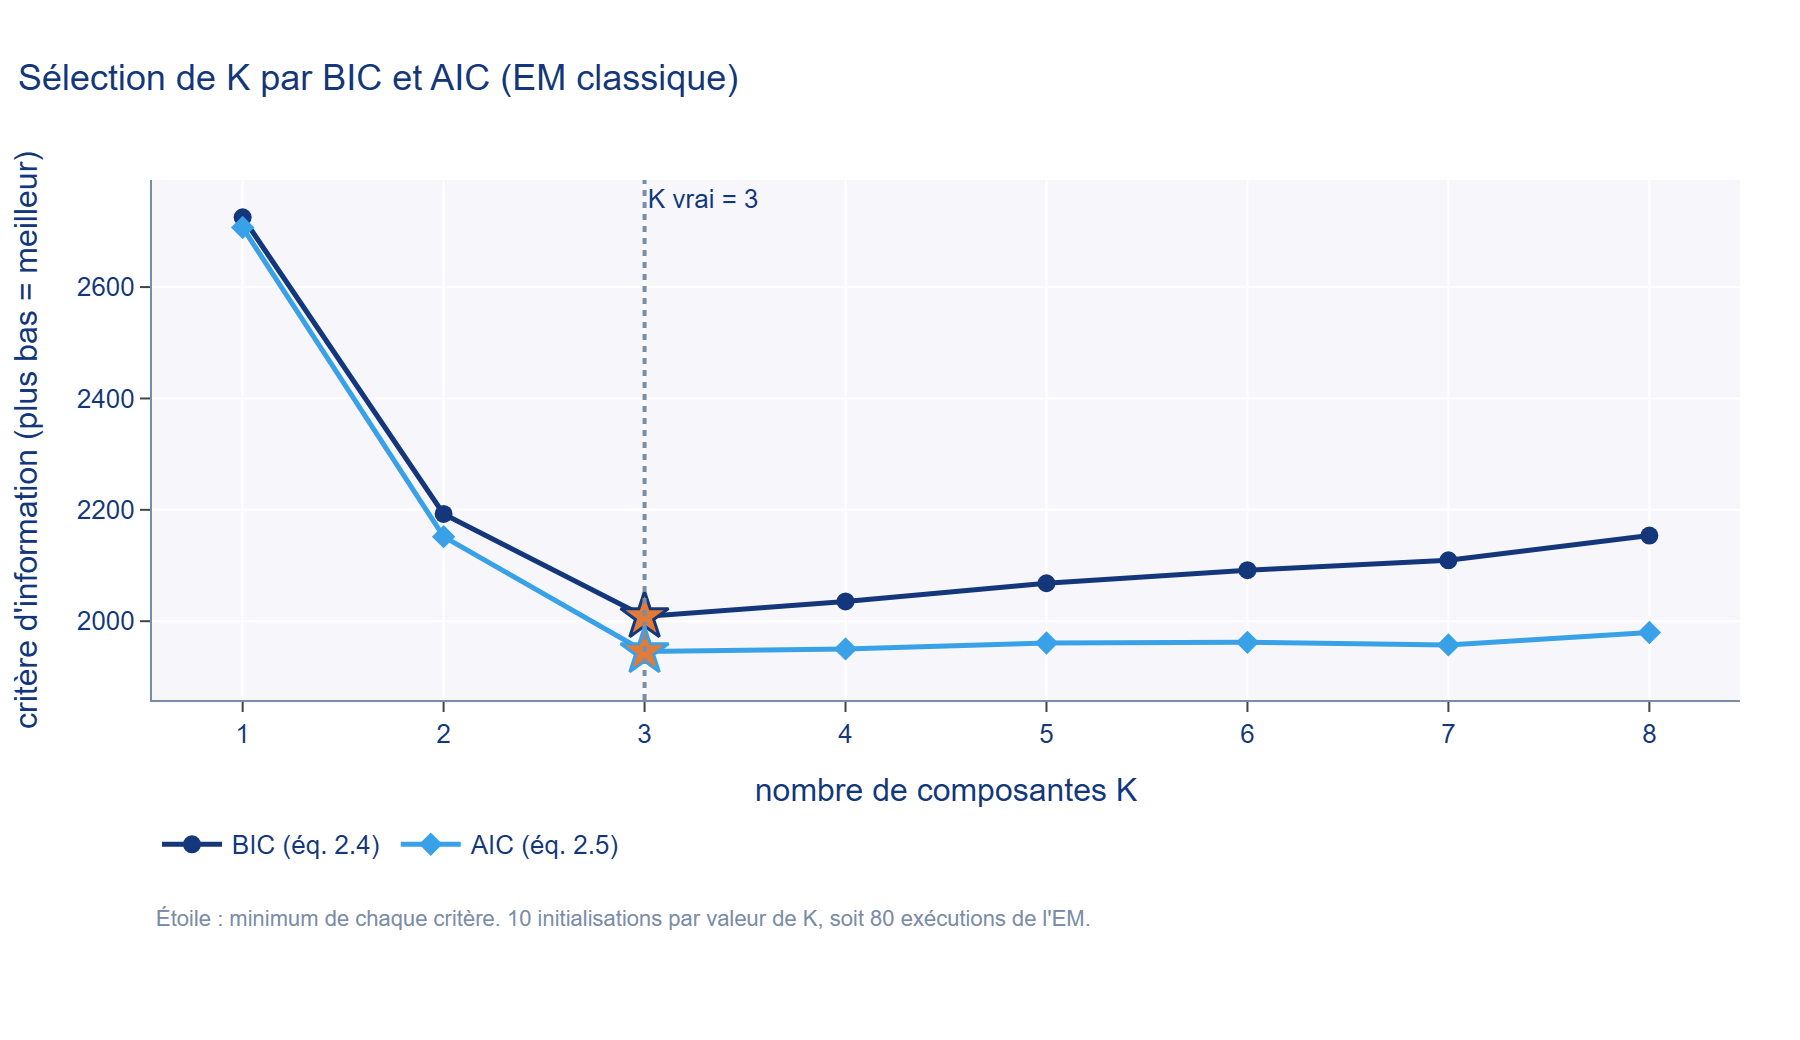
\includegraphics[width=0.85\textwidth]{figures/fig02.png}
\caption{Critères BIC et AIC de l'EM classique en fonction du nombre de composantes K, sur le jeu de données à trois groupes réels.}
\label{fig:2_1}
\end{figure}
Les deux critères atteignent leur minimum exactement à K = 3, ce qui correspond au nombre réel de groupes, confirmant que la procédure de sélection externe par BIC ou AIC fonctionne correctement sur ce jeu de données lorsqu'elle est appliquée avec soin. Ce résultat mérite cependant d'être mis en perspective : l'obtention de la figure 2.1 a nécessité l'exécution complète de l'EM classique pour chacune des huit valeurs de K considérées, soit huit ajustements indépendants (avec, de surcroît, dix initialisations chacun pour éviter les optima locaux, soit quatre-vingts exécutions au total), alors que l'EM variationnel de la section 2.3.3 parvient à une conclusion équivalente  trois composantes actives  en une seule exécution avec Kmax = 6. Ce contraste illustre concrètement l'avantage pratique de la sélection endogène de l'EM variationnel évoqué à la section 2.2.3 ci-dessus : le gain n'est pas seulement conceptuel, il se traduit par un facteur d'économie de calcul proportionnel au nombre de valeurs de K testées lors d'une sélection par BIC ou AIC.

\section{Étude expérimentale}
\subsection{Protocole expérimental}
Afin d'illustrer concrètement les différences de comportement entre l'EM classique et l'EM variationnel mises en évidence sur le plan théorique, nous avons conduit une étude expérimentale fondée sur un jeu de données synthétique bidimensionnel. Ce choix méthodologique permet une visualisation directe des résultats et une interprétation sans ambiguïté des mécanismes en jeu.

Le jeu de données est constitué de N = 300 observations bidimensionnelles, générées à partir de trois groupes gaussiens, de centres respectifs (0, 0), (5, 5) et (0, 5), chacun comportant 100 observations et une covariance isotrope d'écart-type 0,7 (variance 0,49). Les centres sont distants de 5 à 7,1 unités, soit de 7 à 10 écarts-types : les trois groupes sont donc bien séparés. Ce jeu de données constitue, par construction, un mélange à trois composantes gaussiennes. Il est tiré avec la graine 42 ; la section 2.3.13 répète le protocole sur trente jeux indépendants.

L'expérience consiste à ajuster, sur ce même jeu de données, un GMM classique via l'algorithme EM classique et un GMM bayésien via l'algorithme EM variationnel, en imposant dans les deux cas un nombre de composantes délibérément surestimé, K = 6, soit le double du nombre réel de groupes. L'objectif est d'observer comment chacun des deux algorithmes gère cette surestimation. Deux jeux d'hyperparamètres sont considérés pour l'EM variationnel : des priors empiriques (centrés sur les données : $\beta _{0}$ = 1, $W_{0}^{-1}$ égale à la covariance empirique) et des priors diffus ($\beta _{0}$ = $10^{-3}$, $W_{0}$ = I). Sauf mention contraire, les résultats rapportés utilisent les priors empiriques.

\begin{table}[H]
\centering
\small
\setlength{\tabcolsep}{0.14cm}
\begin{tabular}{|p{7.42cm}|p{7.42cm}|}
\hline
\textbf{Paramètre} & \textbf{Valeur} \\
\hline
Nombre d'observations (N) & 300 (3 groupes de 100) \\
\hline
Dimension (D) & 2 \\
\hline
Nombre de composantes imposé (K) & 6 (nombre réel de groupes : 3) \\
\hline
Covariance des groupes générateurs & Isotrope, écart-type 0,7 (variance 0,49) \\
\hline
Graine de génération des données & 42 \\
\hline
EM classique & Mélange gaussien, covariance pleine, initialisation par k-means \\
\hline
EM variationnel & GMM bayésien, covariance pleine, prior de Dirichlet fini de concentration $\alpha _{0}$ \\
\hline
Priors Normal-Wishart (empiriques) & $m_{0}$ = moyenne des données, $\beta _{0}$ = 1, $\nu _{0}$ = D, $W_{0}^{-1}$ = covariance empirique \\
\hline
Concentration du prior de Dirichlet ($\alpha _{0}$) & 1 / K = 0,167 \\
\hline
Critère d'arrêt ($\varepsilon $) & $10^{-3}$ (EM : variation de la log-vraisemblance par observation ; EM variationnel : variation totale de l'ELBO) \\
\hline
Nombre maximal d'itérations & 200 (EM), 500 (EM variationnel) \\
\hline
Nombre d'initialisations & 10 (meilleur critère retenu) \\
\hline
Composante active & $N_{k} = \sum _{i} r_{ik} \geq 1$ \\
\hline
\end{tabular}
\caption{Paramètres du protocole expérimental}
\label{tab:2_4}
\end{table}
\emph{Source : implémentation PyTorch décrite à l'annexe A.}

\begin{figure}[H]
\centering
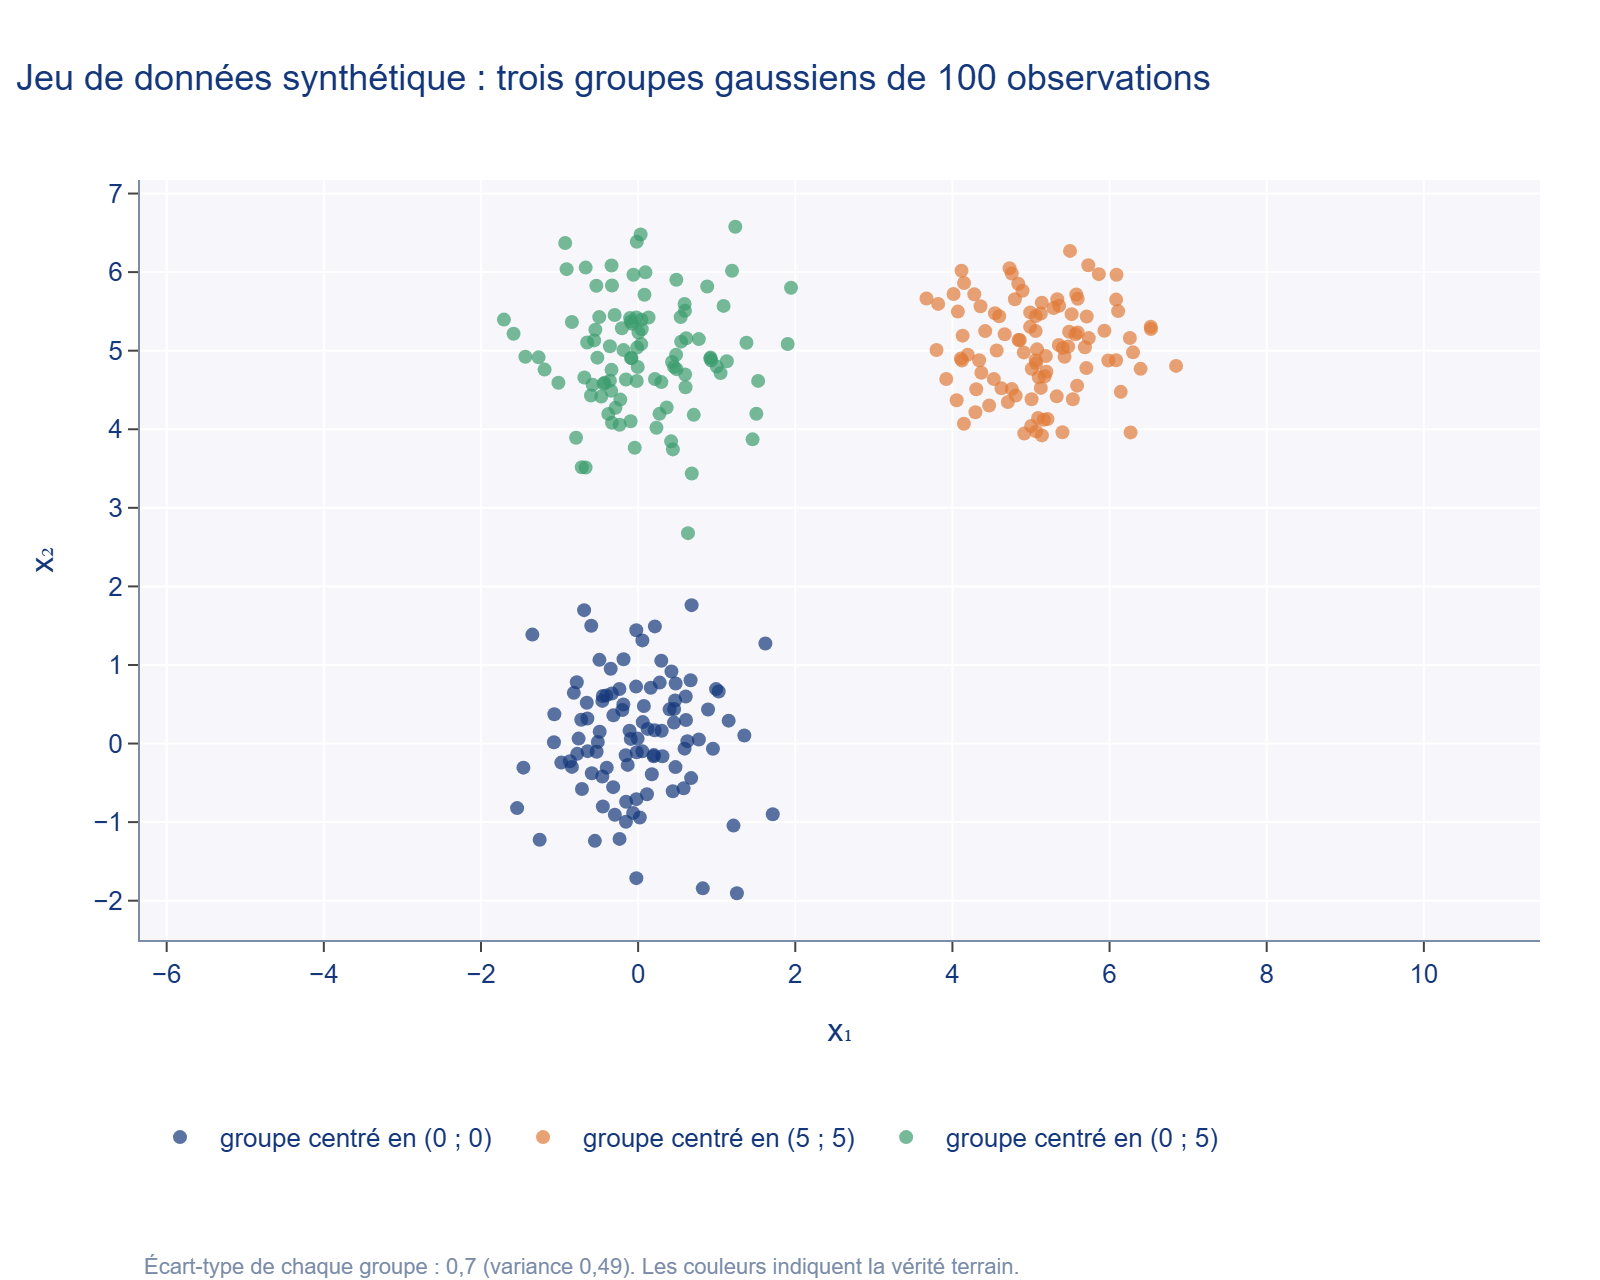
\includegraphics[width=0.85\textwidth]{figures/fig03.png}
\caption{Jeu de données synthétique utilisé pour l'étude expérimentale : trois groupes gaussiens réels de 100 observations chacun (N = 300 au total).}
\label{fig:2_2}
\end{figure}
\subsection{Résultats de l'EM classique (K = 6 imposé)}
L'exécution de l'EM classique avec K = 6 composantes converge en 8 itérations vers une log-vraisemblance totale de -946,00. Le tableau 2.5 présente les poids finaux obtenus pour chacune des six composantes.

\begin{table}[H]
\centering
\small
\setlength{\tabcolsep}{0.09cm}
\begin{tabular}{|p{1.98cm}|p{1.98cm}|p{1.98cm}|p{1.98cm}|p{1.98cm}|p{1.98cm}|p{1.98cm}|}
\hline
\textbf{Composante} & \textbf{1} & \textbf{2} & \textbf{3} & \textbf{4} & \textbf{5} & \textbf{6} \\
\hline
Poids $\pi _{k}$ & 0,333 & 0,013 & 0,167 & 0,148 & 0,185 & 0,154 \\
\hline
\end{tabular}
\caption{Poids de mélange obtenus par l'EM classique (K = 6)}
\label{tab:2_5}
\end{table}
Ce résultat illustre la limite théorique décrite au chapitre 1 : en l'absence de mécanisme de régularisation sur le nombre de composantes, l'EM classique conserve ses six composantes. Le poids le plus faible, 0,013 (soit $N_{k} \approx 4$), reste supérieur au seuil d'activité $N_{k} = 1$ : aucune composante n'est écartée. La composante 1, de poids 0,333, capture à elle seule l'un des trois groupes, tandis que les cinq autres composantes se partagent les deux groupes restants, pourtant bien séparés, en les fragmentant de façon arbitraire (figure 2.3). L'algorithme ne dispose d'aucun mécanisme interne pour reconnaître que K = 6 est surestimé par rapport à la structure réelle des données.

\subsection{Résultats de l'EM variationnel (Kmax = 6)}
L'exécution de l'EM variationnel avec Kmax = 6 composantes, des priors empiriques et un prior de Dirichlet de concentration $\alpha _{0}$ = 1/K converge en 25 itérations vers une ELBO de -1046,62, calculée exactement selon l'équation (1.31). Cette valeur est inférieure à la log-vraisemblance maximale de l'EM classique (-946,00), comme l'exige la chaîne d'inégalités $\mathrm{ELBO} \leq \log p(X) \leq \max _{\theta } \log p(X|\theta )$ : les deux quantités ne mesurent pas la même chose (l'ELBO intègre la pénalité de complexité due aux priors) et ne se comparent pas comme deux scores d'ajustement. Le tableau 2.6 présente les poids finaux obtenus.

\begin{table}[H]
\centering
\small
\setlength{\tabcolsep}{0.09cm}
\begin{tabular}{|p{1.98cm}|p{1.98cm}|p{1.98cm}|p{1.98cm}|p{1.98cm}|p{1.98cm}|p{1.98cm}|}
\hline
\textbf{Composante} & \textbf{1} & \textbf{2} & \textbf{3} & \textbf{4} & \textbf{5} & \textbf{6} \\
\hline
Poids $\pi _{k}$ & 0,001 & 0,335 & 0,331 & 0,333 & 0,001 & 0,001 \\
\hline
\end{tabular}
\caption{Poids de mélange obtenus par l'EM variationnel (Kmax = 6)}
\label{tab:2_6}
\end{table}
Contrairement à l'EM classique, l'EM variationnel identifie nettement trois composantes dominantes, de poids 0,335, 0,331 et 0,333, très proches de la proportion réelle d'un tiers par groupe, tandis que les trois composantes restantes voient leur poids s'effondrer à 0,001, soit un nombre effectif de points assignés $N_{k} \approx 0,3$, en deçà du seuil d'activité $N_{k} < 1$ défini à la section 1.7.4. Ces trois dernières composantes sont donc éteintes et le modèle final ne conserve que trois composantes actives, en adéquation avec la structure du jeu de données, alors même que l'algorithme n'a jamais reçu cette information en entrée. La figure 2.3 illustre ce contraste : les ellipses de covariance de l'EM classique se répartissent de façon désordonnée sur deux des groupes, tandis que celles de l'EM variationnel épousent les trois groupes réels.

Ce résultat dépend des priors. Avec les priors diffus ($\beta _{0}$ = $10^{-3}$, $W_{0}$ = I), la même expérience conserve quatre composantes actives (poids 0,326 ; 0,333 ; 0,332 et 0,008, ARI de 0,985) et demande 103 itérations. La section 2.3.13 quantifie cette dépendance sur trente jeux de données.

\begin{figure}[H]
\centering
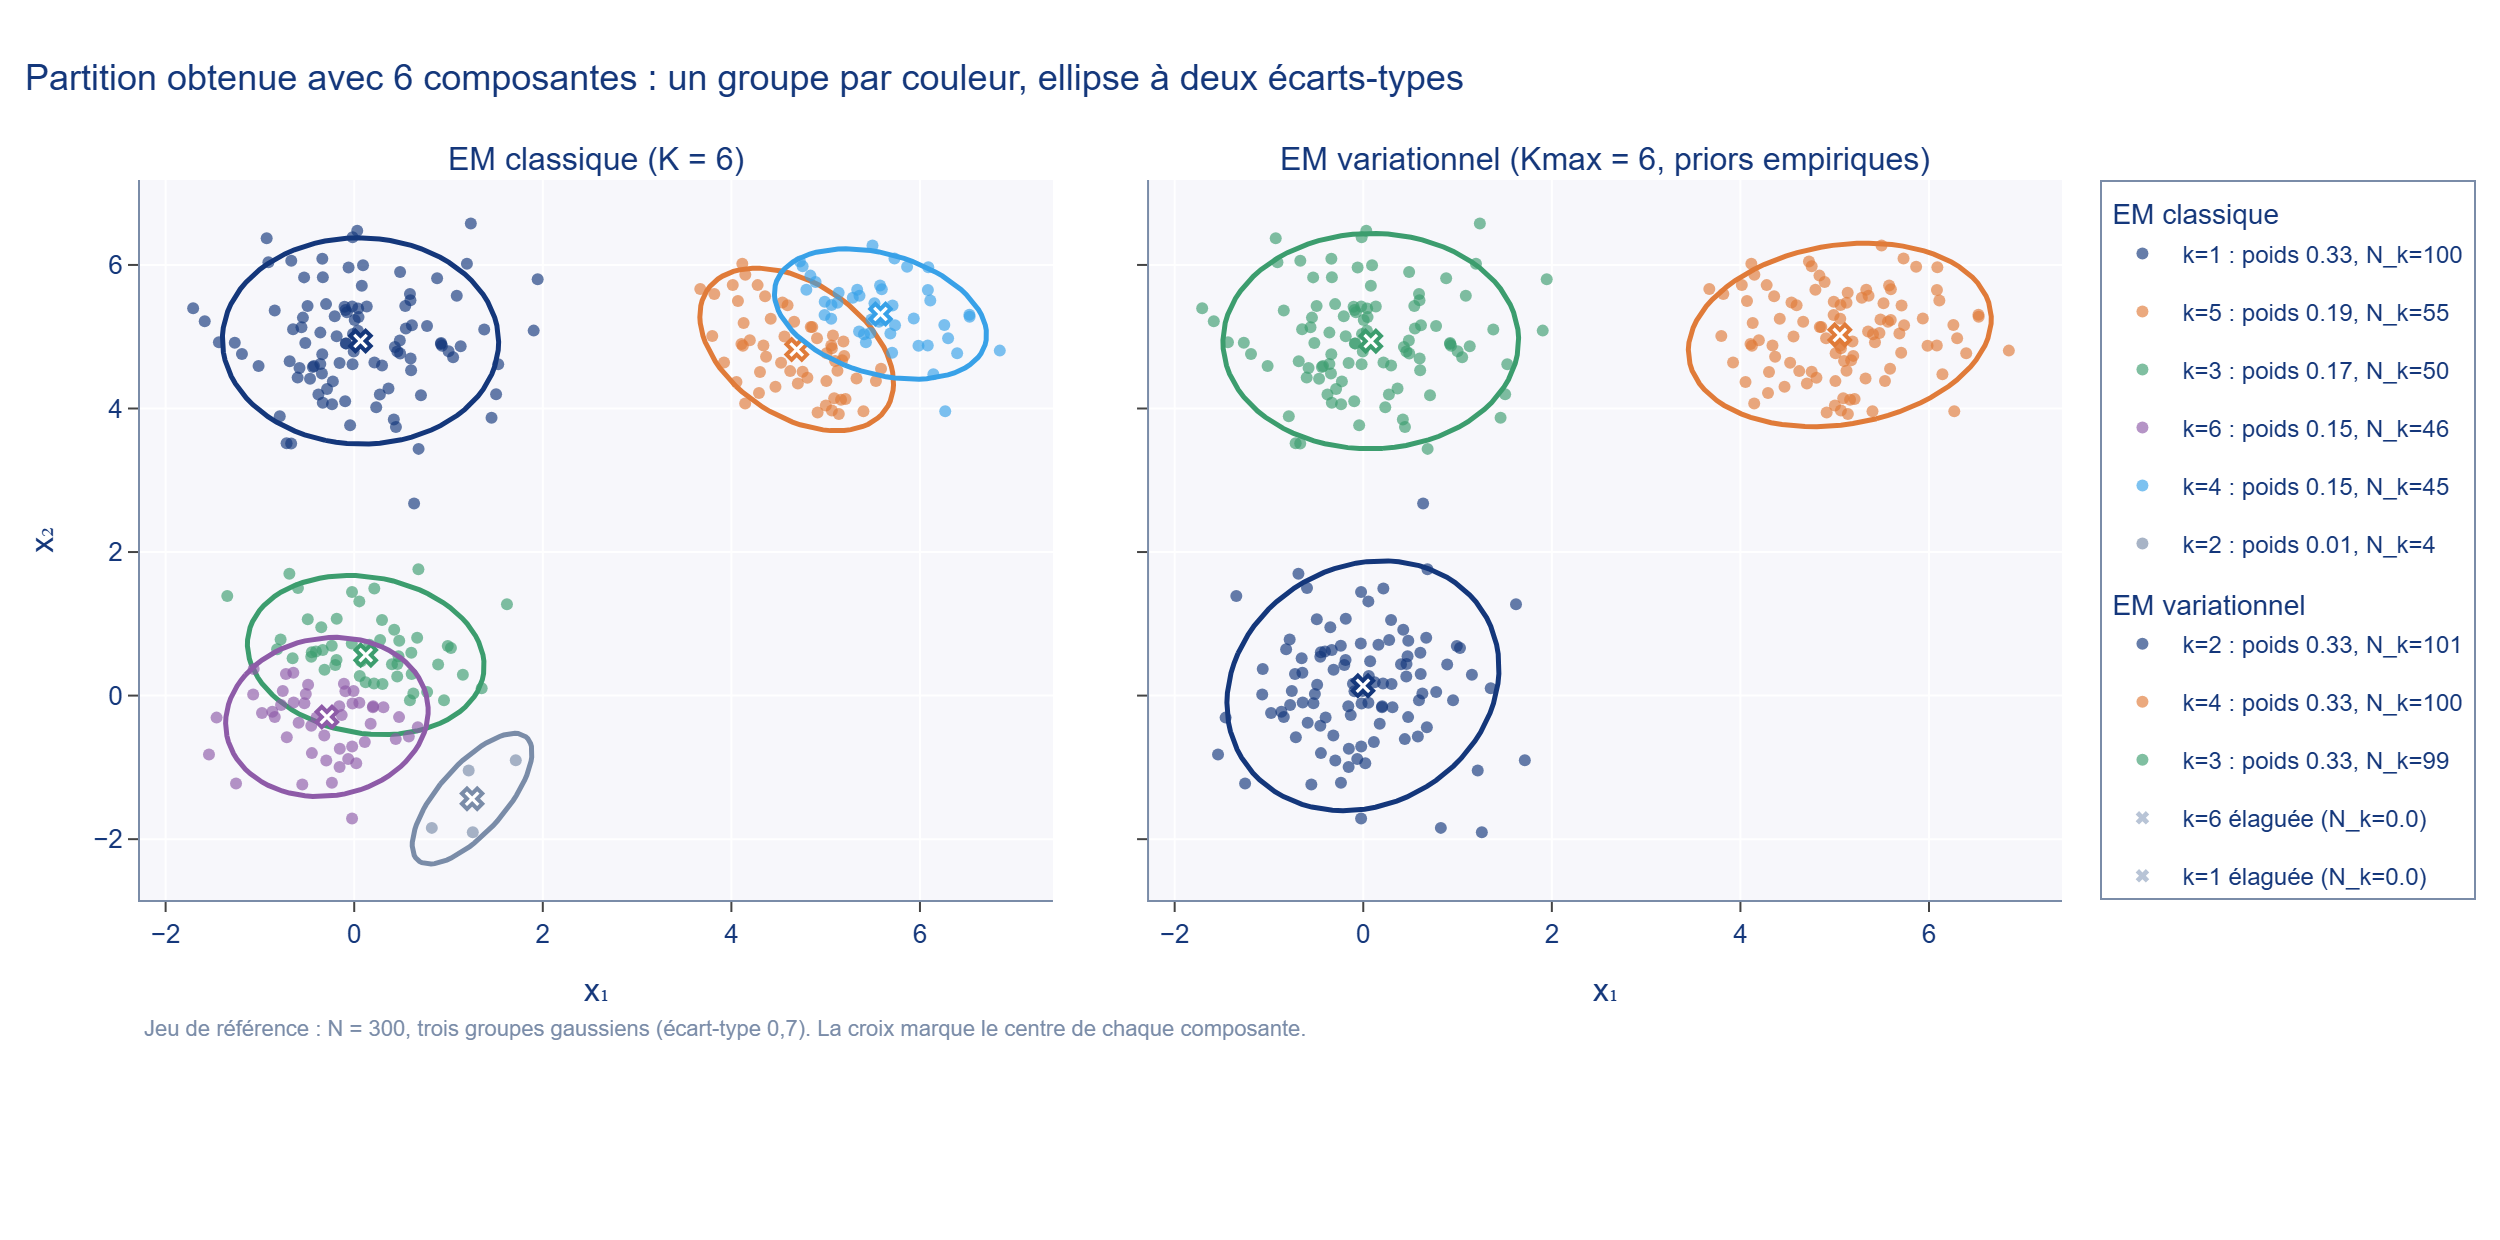
\includegraphics[width=0.95\textwidth]{figures/fig04.png}
\caption{Partition obtenue avec six composantes : une couleur par composante, ellipses de covariance à deux écarts-types, croix aux centres. À gauche, l'EM classique conserve ses six composantes ; à droite, l'EM variationnel n'en retient que trois (les composantes élaguées figurent en gris dans la légende).}
\label{fig:2_3}
\end{figure}
\begin{figure}[H]
\centering
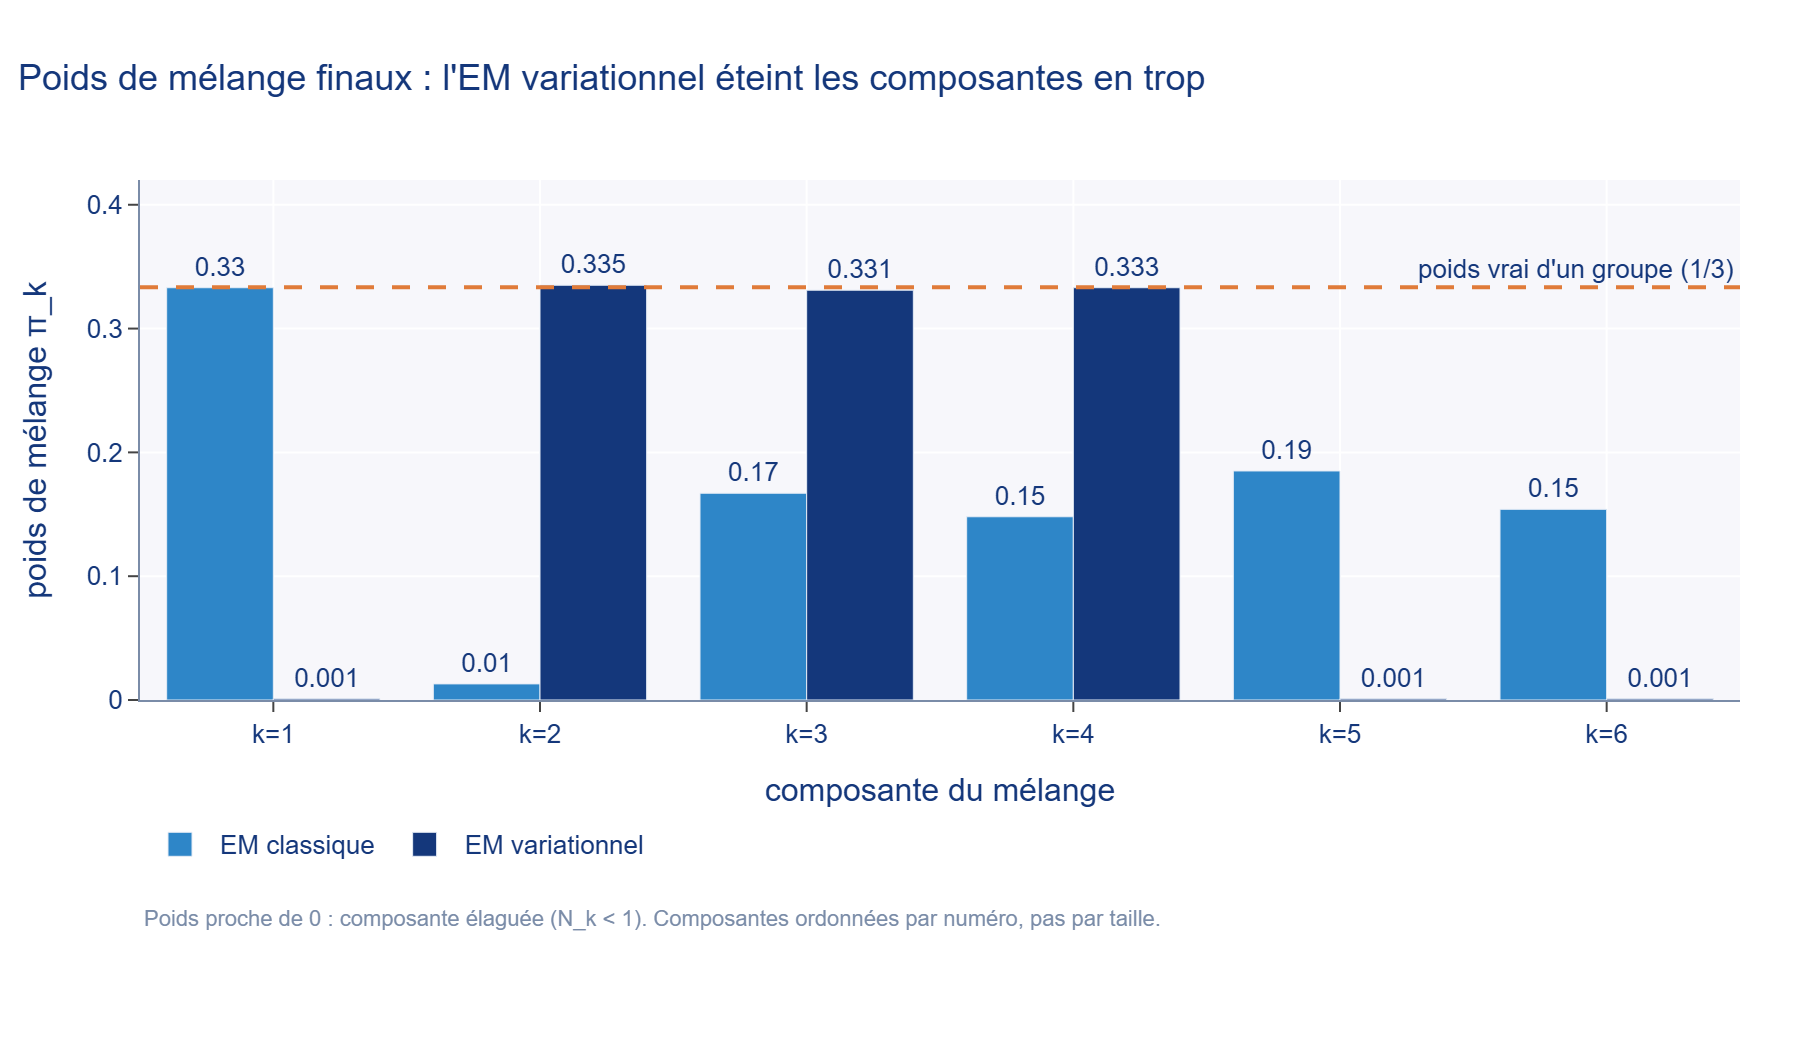
\includegraphics[width=0.85\textwidth]{figures/fig05.png}
\caption{Poids de mélange $\pi _{k}$ finaux pour les six composantes : EM classique et EM variationnel. Le contraste traduit le mécanisme d'élagage bayésien décrit à la section 1.7.4.}
\label{fig:2_4}
\end{figure}
\subsection{Comparaison visuelle et qualité de partition}
Au-delà des poids de mélange, la qualité des partitions obtenues par les deux algorithmes peut être évaluée à l'aide de métriques externes de clustering, en comparant les affectations produites aux véritables étiquettes de groupe. Le tableau 2.7 présente les résultats obtenus pour l'indice de Rand ajusté (ARI) et le score de silhouette, calculés sur les affectations dures obtenues en prenant, pour chaque observation, la composante de responsabilité maximale.

\begin{table}[H]
\centering
\small
\setlength{\tabcolsep}{0.14cm}
\begin{tabular}{|p{4.84cm}|p{4.84cm}|p{4.84cm}|}
\hline
\textbf{Métrique} & \textbf{EM classique} & \textbf{EM variationnel} \\
\hline
Nombre de composantes effectivement actives & 6 & 3 \\
\hline
Indice de Rand ajusté (ARI) & 0,715 & 0,990 \\
\hline
Score de silhouette moyen & 0,450 & 0,739 \\
\hline
Nombre d'itérations jusqu'à convergence & 8 & 25 \\
\hline
Temps moyen d'exécution (10 initialisations, 30 jeux) & 0,21 s & 0,98 s \\
\hline
\end{tabular}
\caption{Métriques de qualité de partition (K = 6 imposé)}
\label{tab:2_7}
\end{table}
\emph{Source : implémentation PyTorch (graine 42). Les temps sont des moyennes sur les 30 jeux de la section 2.3.13.}

Ces résultats appellent plusieurs commentaires. Premièrement, l'indice de Rand ajusté atteint 0,990 pour l'EM variationnel, c'est-à-dire une partition quasi identique aux trois groupes ayant servi à générer les données (seules quelques observations de frontière sont affectées différemment), sans qu'aucune information sur le nombre réel de groupes n'ait été fournie, si ce n'est la borne supérieure Kmax = 6. L'EM classique, avec un ARI de 0,715, produit une partition nettement moins fidèle, ses six composantes fragmentant artificiellement les groupes réels. Deuxièmement, le score de silhouette, qui mesure la cohésion interne et la séparation des clusters indépendamment de toute étiquette de référence, confirme ce constat : 0,739 pour l'EM variationnel contre 0,450 pour l'EM classique. Troisièmement, le nombre d'itérations est environ trois fois plus élevé pour l'EM variationnel (25 contre 8) et le temps d'exécution environ 4,7 fois supérieur, ce qui illustre le compromis computationnel identifié à la section 2.2.1. Le nombre d'itérations dépend toutefois de la normalisation du critère d'arrêt (par observation pour l'EM, totale pour l'EM variationnel) et ne doit pas être lu comme une propriété intrinsèque des algorithmes.

\subsection{Sensibilité au choix du prior de Dirichlet ($\alpha _{0}$)}
La section 1.7.4 a montré, sur le plan théorique, que le paramètre de concentration $\alpha _{0}$ du prior de Dirichlet contrôle l'intensité du mécanisme d'élagage automatique : plus $\alpha _{0}$ est petit, plus le prior favorise les solutions parcimonieuses. Afin de vérifier empiriquement cette prédiction, nous avons répété l'expérience de la section 2.3.3 en faisant varier $\alpha _{0}$ sur une grille logarithmique \{0,001 ; 0,01 ; 0,1 ; 1 ; 10\}, toutes choses égales par ailleurs (Kmax = 6, mêmes données, dix initialisations), pour les deux jeux de priors. Le tableau 2.8 et la figure 2.5 présentent les résultats obtenus.

\begin{table}[H]
\centering
\small
\setlength{\tabcolsep}{0.09cm}
\begin{tabular}{|p{4.1cm}|p{1.9cm}|p{1.9cm}|p{1.9cm}|p{1.9cm}|p{1.9cm}|}
\hline
\textbf{$\alpha _{0}$} & \textbf{0,001} & \textbf{0,01} & \textbf{0,1} & \textbf{1} & \textbf{10} \\
\hline
Composantes actives, priors empiriques & 3 & 3 & 3 & 3 & 6 \\
\hline
Composantes actives, priors diffus & 3 & 3 & 3 & 4 & 6 \\
\hline
ARI, priors empiriques & 0,990 & 0,990 & 0,990 & 0,990 & 0,960 \\
\hline
ARI, priors diffus & 1,000 & 1,000 & 1,000 & 0,981 & 0,618 \\
\hline
\end{tabular}
\caption{Nombre de composantes actives ($N_{k}$ $\geq $ 1) et ARI en fonction de la concentration $\alpha _{0}$ du prior de Dirichlet}
\label{tab:2_8}
\end{table}
\begin{figure}[H]
\centering
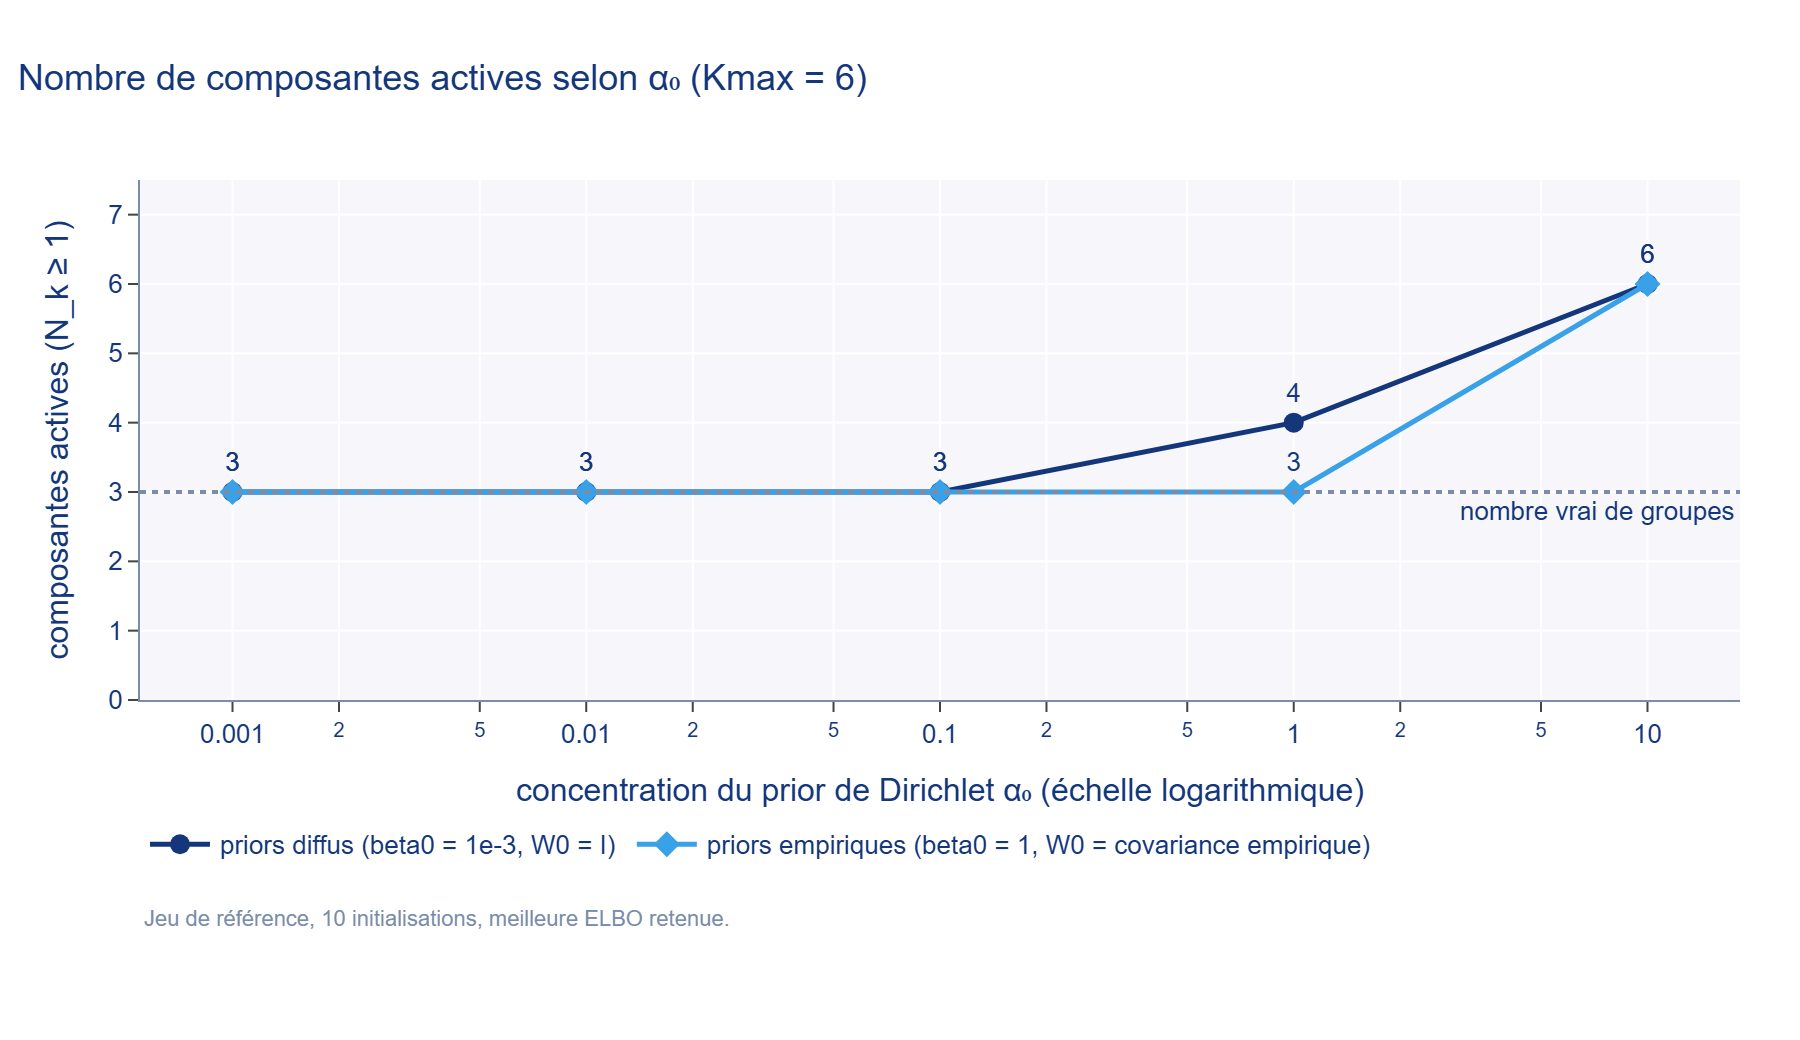
\includegraphics[width=0.85\textwidth]{figures/fig06.png}
\caption{Nombre de composantes actives en fonction de la concentration $\alpha _{0}$ du prior de Dirichlet (échelle logarithmique), pour les deux jeux de priors. Le mécanisme d'élagage disparaît lorsque $\alpha _{0}$ devient grand.}
\label{fig:2_5}
\end{figure}
Ces résultats confirment la prédiction théorique : pour $\alpha _{0} \leq 0,1$, l'algorithme identifie exactement trois composantes actives avec les deux jeux de priors. L'élagage disparaît lorsque $\alpha _{0}$ atteint 10 : les six composantes redeviennent actives et la qualité de la partition se dégrade (ARI de 0,960 avec les priors empiriques, 0,618 avec les priors diffus). Le comportement à $\alpha _{0}$ = 1, concentration pour laquelle le prior de Dirichlet est uniforme et n'encode plus de préférence pour la parcimonie, est plus nuancé que ne le laissait attendre la théorie : l'élagage persiste (trois composantes actives avec les priors empiriques, quatre avec les priors diffus). Le prior de Dirichlet n'est donc pas le seul mécanisme à l'œuvre ; le prior Normal-Wishart contribue lui aussi à pénaliser les composantes superflues, par le terme de divergence de Kullback-Leibler de l'ELBO (équation 1.22), interprétation compatible avec ces observations mais non testée isolément ici. Pour le praticien, $\alpha _{0}$ reste un véritable levier de contrôle de la parcimonie, qu'il convient de fixer à une valeur faible (typiquement $\alpha _{0}$ = 1/Kmax ou inférieure) si l'objectif est la sélection automatique du nombre de composantes.

\subsection{Étude de la scalabilité computationnelle}
Afin de quantifier le surcoût computationnel de l'EM variationnel identifié sur le plan théorique à la section 2.2.1, nous avons mesuré le temps d'exécution des deux algorithmes en faisant varier, d'une part, le nombre d'observations N (à dimension D = 2 fixée), et d'autre part, la dimension D (à N = 2000 fixé), avec trois initialisations et au plus 100 itérations par ajustement. Le tableau 2.9 et la figure 2.6 présentent les résultats obtenus.

\begin{table}[H]
\centering
\small
\setlength{\tabcolsep}{0.14cm}
\begin{tabular}{|p{2.77cm}|p{2.77cm}|p{2.77cm}|p{2.77cm}|p{2.77cm}|}
\hline
\textbf{Paramètre variable} & \textbf{Valeur} & \textbf{EM classique (s)} & \textbf{EM variationnel (s)} & \textbf{Ratio (var./class.)} \\
\hline
N (D=2) & 300 & 0,123 & 0,839 & 6,8 \\
\hline
N (D=2) & 1 000 & 0,120 & 1,390 & 11,6 \\
\hline
N (D=2) & 5 000 & 0,420 & 2,377 & 5,7 \\
\hline
N (D=2) & 20 000 & 0,856 & 4,102 & 4,8 \\
\hline
D (N=2000) & 2 & 0,207 & 1,717 & 8,3 \\
\hline
D (N=2000) & 5 & 0,182 & 1,504 & 8,3 \\
\hline
D (N=2000) & 10 & 0,202 & 1,476 & 7,3 \\
\hline
D (N=2000) & 20 & 0,481 & 1,122 & 2,3 \\
\hline
\end{tabular}
\caption{Temps d'exécution (en secondes) en fonction de N et de D}
\label{tab:2_9}
\end{table}
\begin{figure}[H]
\centering
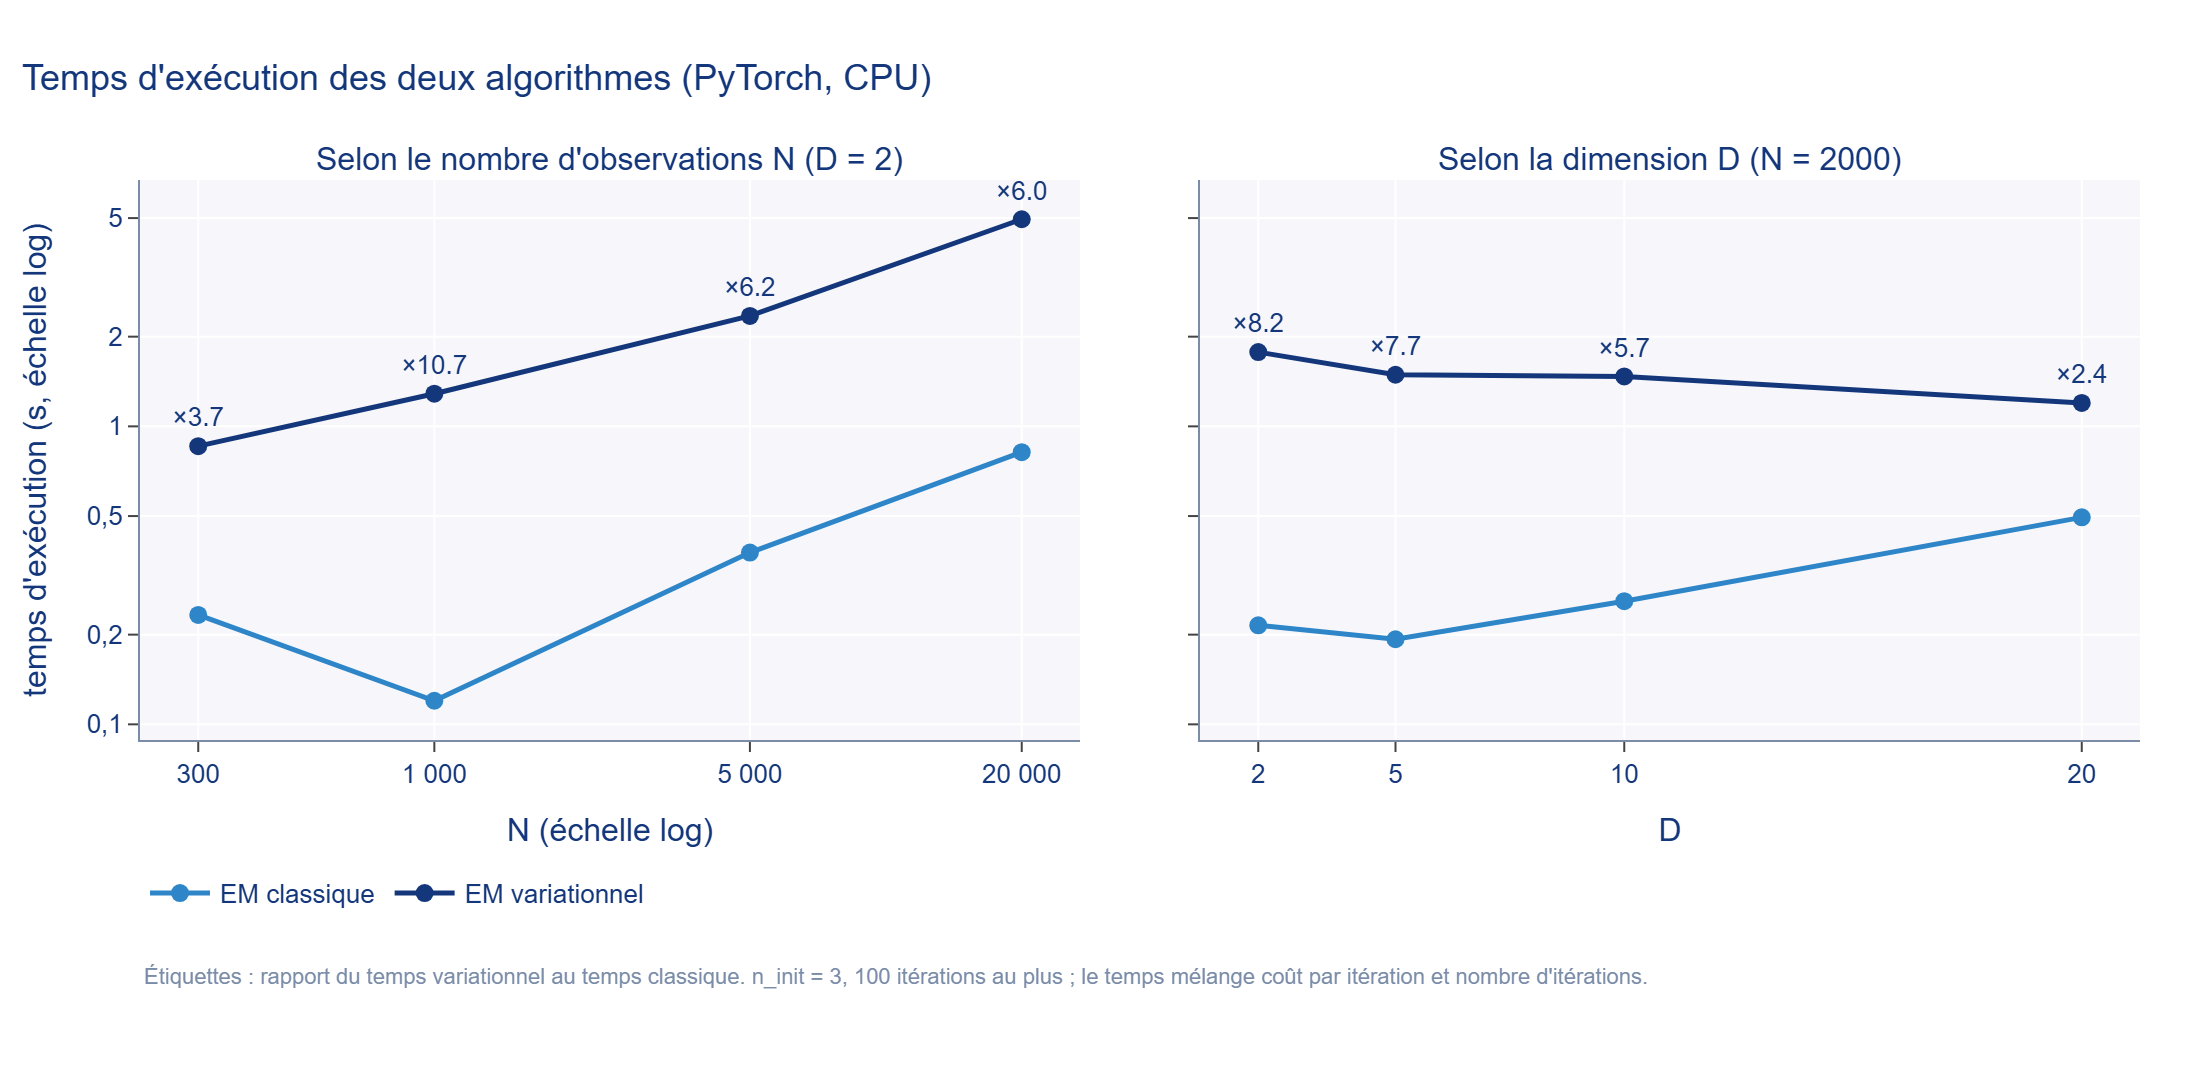
\includegraphics[width=0.95\textwidth]{figures/fig07.png}
\caption{Temps d'exécution des deux algorithmes en fonction du nombre d'observations N (à gauche, échelles logarithmiques) et de la dimension D (à droite). Les étiquettes donnent le rapport du temps variationnel au temps classique.}
\label{fig:2_6}
\end{figure}
\emph{Source : implémentation PyTorch (CPU, machine unique, graine 42).}

Ces mesures confirment que l'EM variationnel demeure plus coûteux que l'EM classique, avec un facteur multiplicatif compris entre 2,3 et 11,6 selon les régimes. Le rapport tend à diminuer lorsque N ou D augmente (de 8,3 à D = 2 à 2,3 à D = 20 ; de 6,8 à N = 300 à 4,8 à N = 20 000). Ce comportement est cohérent avec l'analyse de complexité de la section 2.2.1 : le terme en $KD^{3}$, commun aux deux algorithmes, finit par dominer le calcul et resserre l'écart relatif. Les temps mesurés combinent toutefois le coût par itération et le nombre d'itérations, qui n'est pas contrôlé, et la mesure unique par configuration est bruitée (le temps de l'EM classique à N = 1 000 est ainsi égal à celui mesuré à N = 300). En valeur absolue, les deux algorithmes restent d'un coût raisonnable sur les tailles considérées (environ 4 secondes pour 20 000 observations), et le choix entre eux devrait être dicté davantage par la qualité de la solution recherchée que par cette seule considération de temps de calcul.

\subsection{Cas de référence : nombre de composantes correctement spécifié (K = 3)}
L'ensemble des résultats précédents portent sur le cas, volontairement défavorable à l'EM classique, où le nombre de composantes est surestimé. Afin de vérifier que les deux algorithmes se comportent de façon équivalente lorsque cette surestimation est absente, nous avons répété l'expérience avec K = 3, c'est-à-dire avec le nombre exact de groupes réels du jeu de données. Le tableau 2.10 présente les résultats obtenus.

\begin{table}[H]
\centering
\small
\setlength{\tabcolsep}{0.14cm}
\begin{tabular}{|p{4.84cm}|p{4.84cm}|p{4.84cm}|}
\hline
\textbf{Métrique} & \textbf{EM classique} & \textbf{EM variationnel} \\
\hline
Poids de mélange & 0,333 / 0,334 / 0,332 & 0,333 / 0,335 / 0,331 \\
\hline
Indice de Rand ajusté (ARI) & 1,000 & 0,990 \\
\hline
Score de silhouette & 0,740 & 0,739 \\
\hline
Nombre d'itérations & 2 & 4 \\
\hline
\end{tabular}
\caption{Résultats de référence avec le nombre de composantes correctement spécifié (K = 3)}
\label{tab:2_10}
\end{table}
Ce cas de référence est riche d'enseignement : lorsque le nombre de composantes est correctement spécifié, les deux algorithmes convergent en 2 et 4 itérations vers des solutions quasi identiques (ARI de 1,000 et 0,990, silhouettes de 0,740 et 0,739). L'écart d'ARI correspond à la régularisation exercée par les priors sur les observations de frontière. Ce résultat confirme que la supériorité de l'EM variationnel observée aux sections 2.3.3 et 2.3.4 n'est pas une propriété intrinsèque qui le rendrait préférable en toute circonstance ; elle ne se manifeste que lorsque le nombre réel de composantes est inconnu et que le nombre utilisé pour l'ajustement s'en écarte. Ce constat rejoint la synthèse théorique du tableau 2.1 : le choix entre les deux algorithmes doit être guidé par le degré de confiance dont dispose le praticien quant au nombre réel de composantes sous-jacentes à ses données.

\subsection{Convergence de l'ELBO}
La section 1.7.6 a établi que l'ELBO constitue, pour l'EM variationnel, un critère de convergence croissant et borné. Afin d'illustrer cette propriété sur notre étude de cas, la figure 2.7 retrace l'évolution de l'ELBO, calculée exactement à chaque itération selon l'équation (1.31), pour le modèle à Kmax = 6 composantes de la section 2.3.3, avec un critère d'arrêt de $10^{-6}$. Elle présente aussi la log-vraisemblance de l'EM classique pour K = 6.

\begin{figure}[H]
\centering
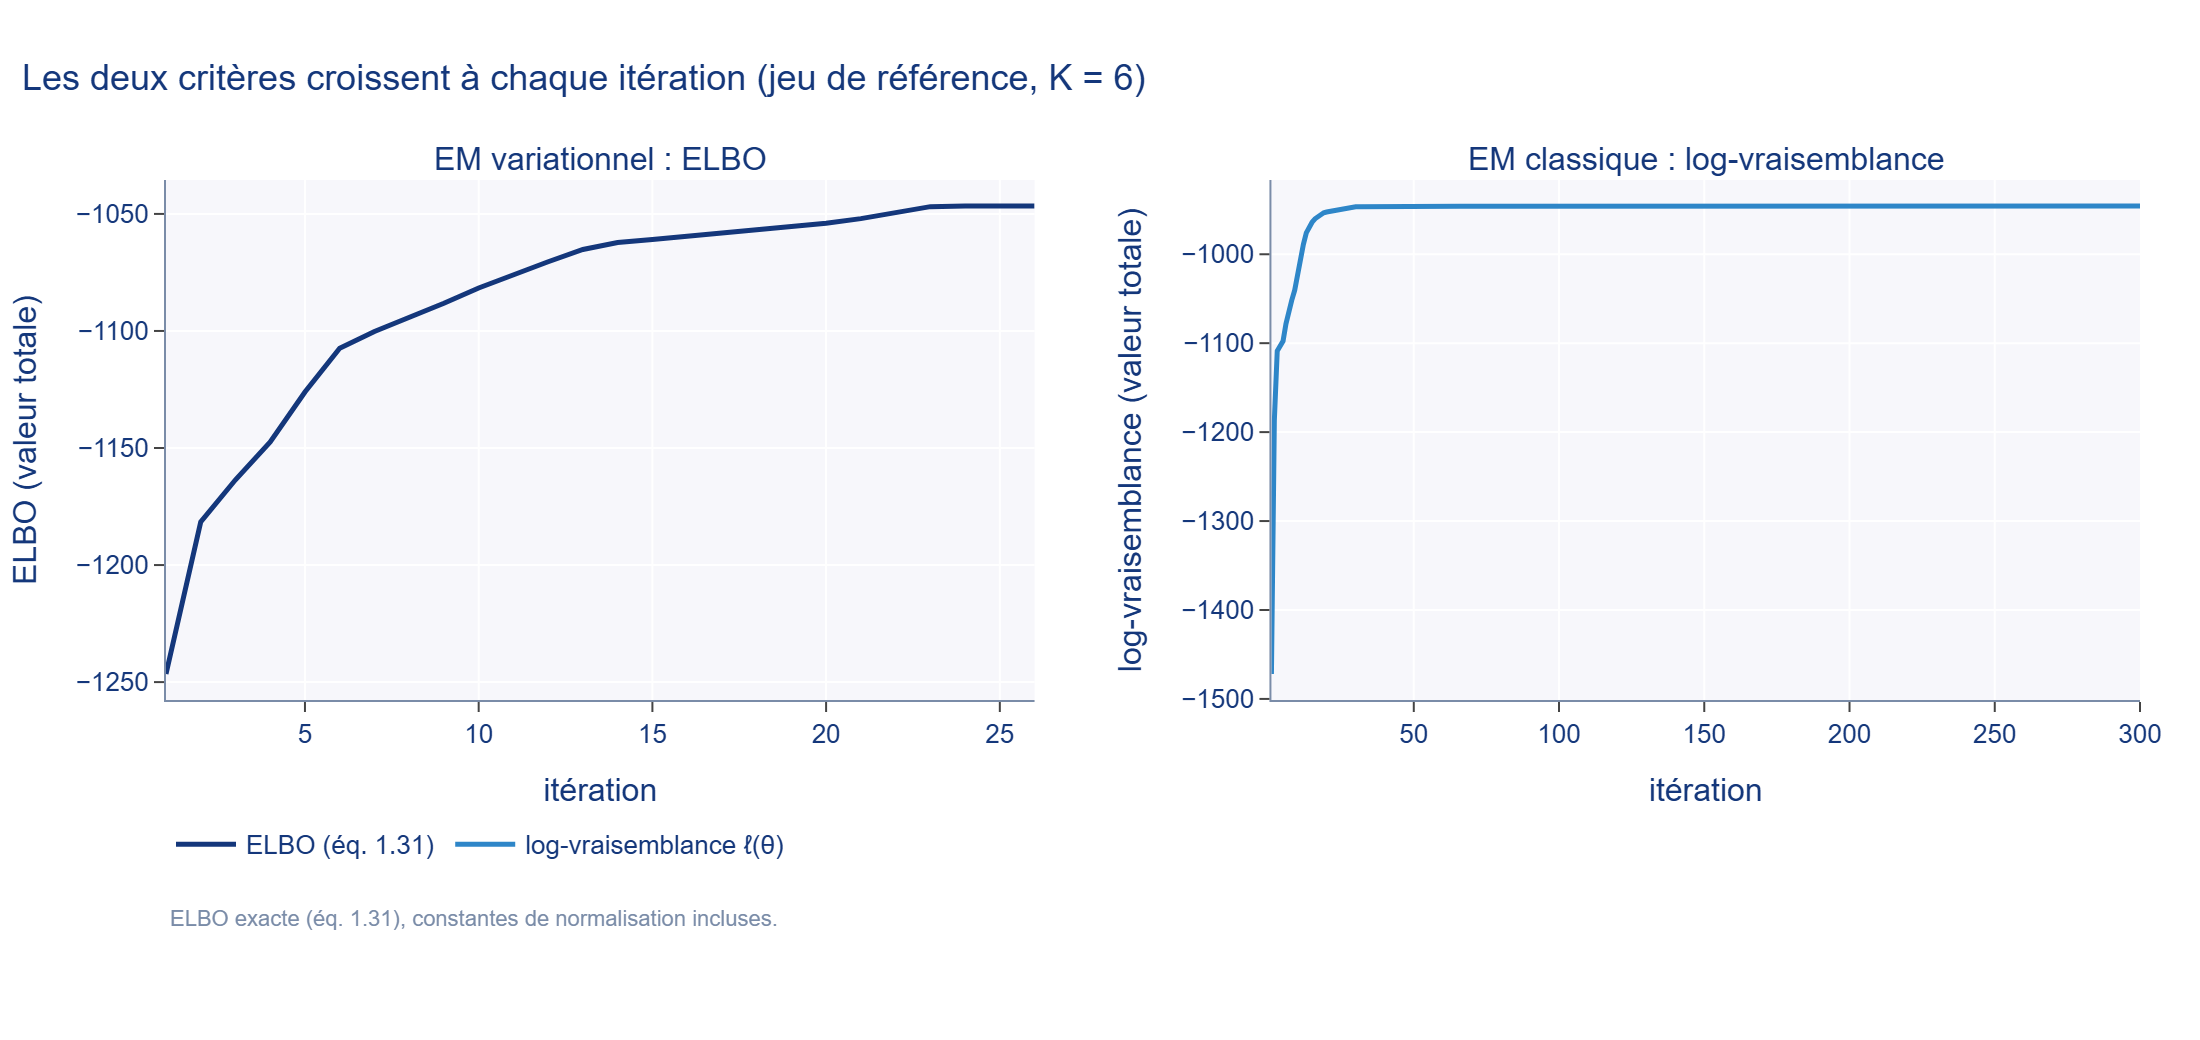
\includegraphics[width=0.95\textwidth]{figures/fig08.png}
\caption{Évolution de l'ELBO (EM variationnel, à gauche) et de la log-vraisemblance (EM classique, à droite) en fonction du nombre d'itérations. Les deux courbes sont croissantes, conformément aux garanties théoriques des sections 1.6.2.f et 1.7.6.}
\label{fig:2_7}
\end{figure}
On observe une croissance strictement monotone de l'ELBO, qui passe de -1246,54 à la première itération à -1046,62 à convergence (26 itérations), sans jamais décroître, conformément à la garantie théorique de la section 1.7.6. Cette monotonie a été vérifiée numériquement à chaque itération, de même que l'inégalité $\mathrm{ELBO} \leq \log p(X) \leq \ell (\hat{\theta })$ et l'égalité de Neal et Hinton, $F(q^{*},\theta ) = \ell (\theta )$ après l'étape E, vérifiée à $10^{-13}$ près. La forme de la courbe, avec une phase de croissance rapide suivie d'un plateau, est typique des algorithmes de type EM : les premières itérations réorganisent grossièrement les responsabilités entre composantes, tandis que les dernières itérations affinent marginalement les paramètres sans modifier l'affectation qualitative des observations.

\subsection{Robustesse à l'initialisation}
L'ensemble des résultats précédents ont été obtenus avec dix initialisations indépendantes, dont la meilleure solution est conservée, pratique recommandée pour se prémunir contre la convergence vers un optimum local médiocre (sections 1.6.3.a et 1.7.9). Afin de quantifier la sensibilité propre de chaque algorithme à l'initialisation, nous avons répété l'expérience de la section 2.3.1 avec une seule initialisation par exécution, pour 20 graines indépendantes et deux stratégies : initialisation par k-means, et initialisation aléatoire (K points de données tirés au hasard, section 1.6.2.a pour l'EM classique et section 1.7.3.d pour l'EM variationnel).

\begin{table}[H]
\centering
\small
\setlength{\tabcolsep}{0.14cm}
\begin{tabular}{|p{2.2cm}|p{4.5cm}|p{1.6cm}|p{1.6cm}|p{1.6cm}|p{1.6cm}|}
\hline
\textbf{Initialisation} & \textbf{Algorithme} & \textbf{3 actives} & \textbf{4 actives} & \textbf{5 actives} & \textbf{6 actives} \\
\hline
k-means & EM classique & 0 / 20 & 0 / 20 & 0 / 20 & 20 / 20 \\
\hline
k-means & EM variationnel, priors diffus & 0 / 20 & 12 / 20 & 8 / 20 & 0 / 20 \\
\hline
k-means & EM variationnel, priors empiriques & 20 / 20 & 0 / 20 & 0 / 20 & 0 / 20 \\
\hline
aléatoire & EM classique & 0 / 20 & 1 / 20 & 1 / 20 & 18 / 20 \\
\hline
aléatoire & EM variationnel, priors diffus & 4 / 20 & 14 / 20 & 2 / 20 & 0 / 20 \\
\hline
aléatoire & EM variationnel, priors empiriques & 20 / 20 & 0 / 20 & 0 / 20 & 0 / 20 \\
\hline
\end{tabular}
\caption{Nombre de composantes actives obtenu sur 20 initialisations indépendantes (une initialisation par exécution)}
\label{tab:2_11}
\end{table}
\begin{figure}[H]
\centering
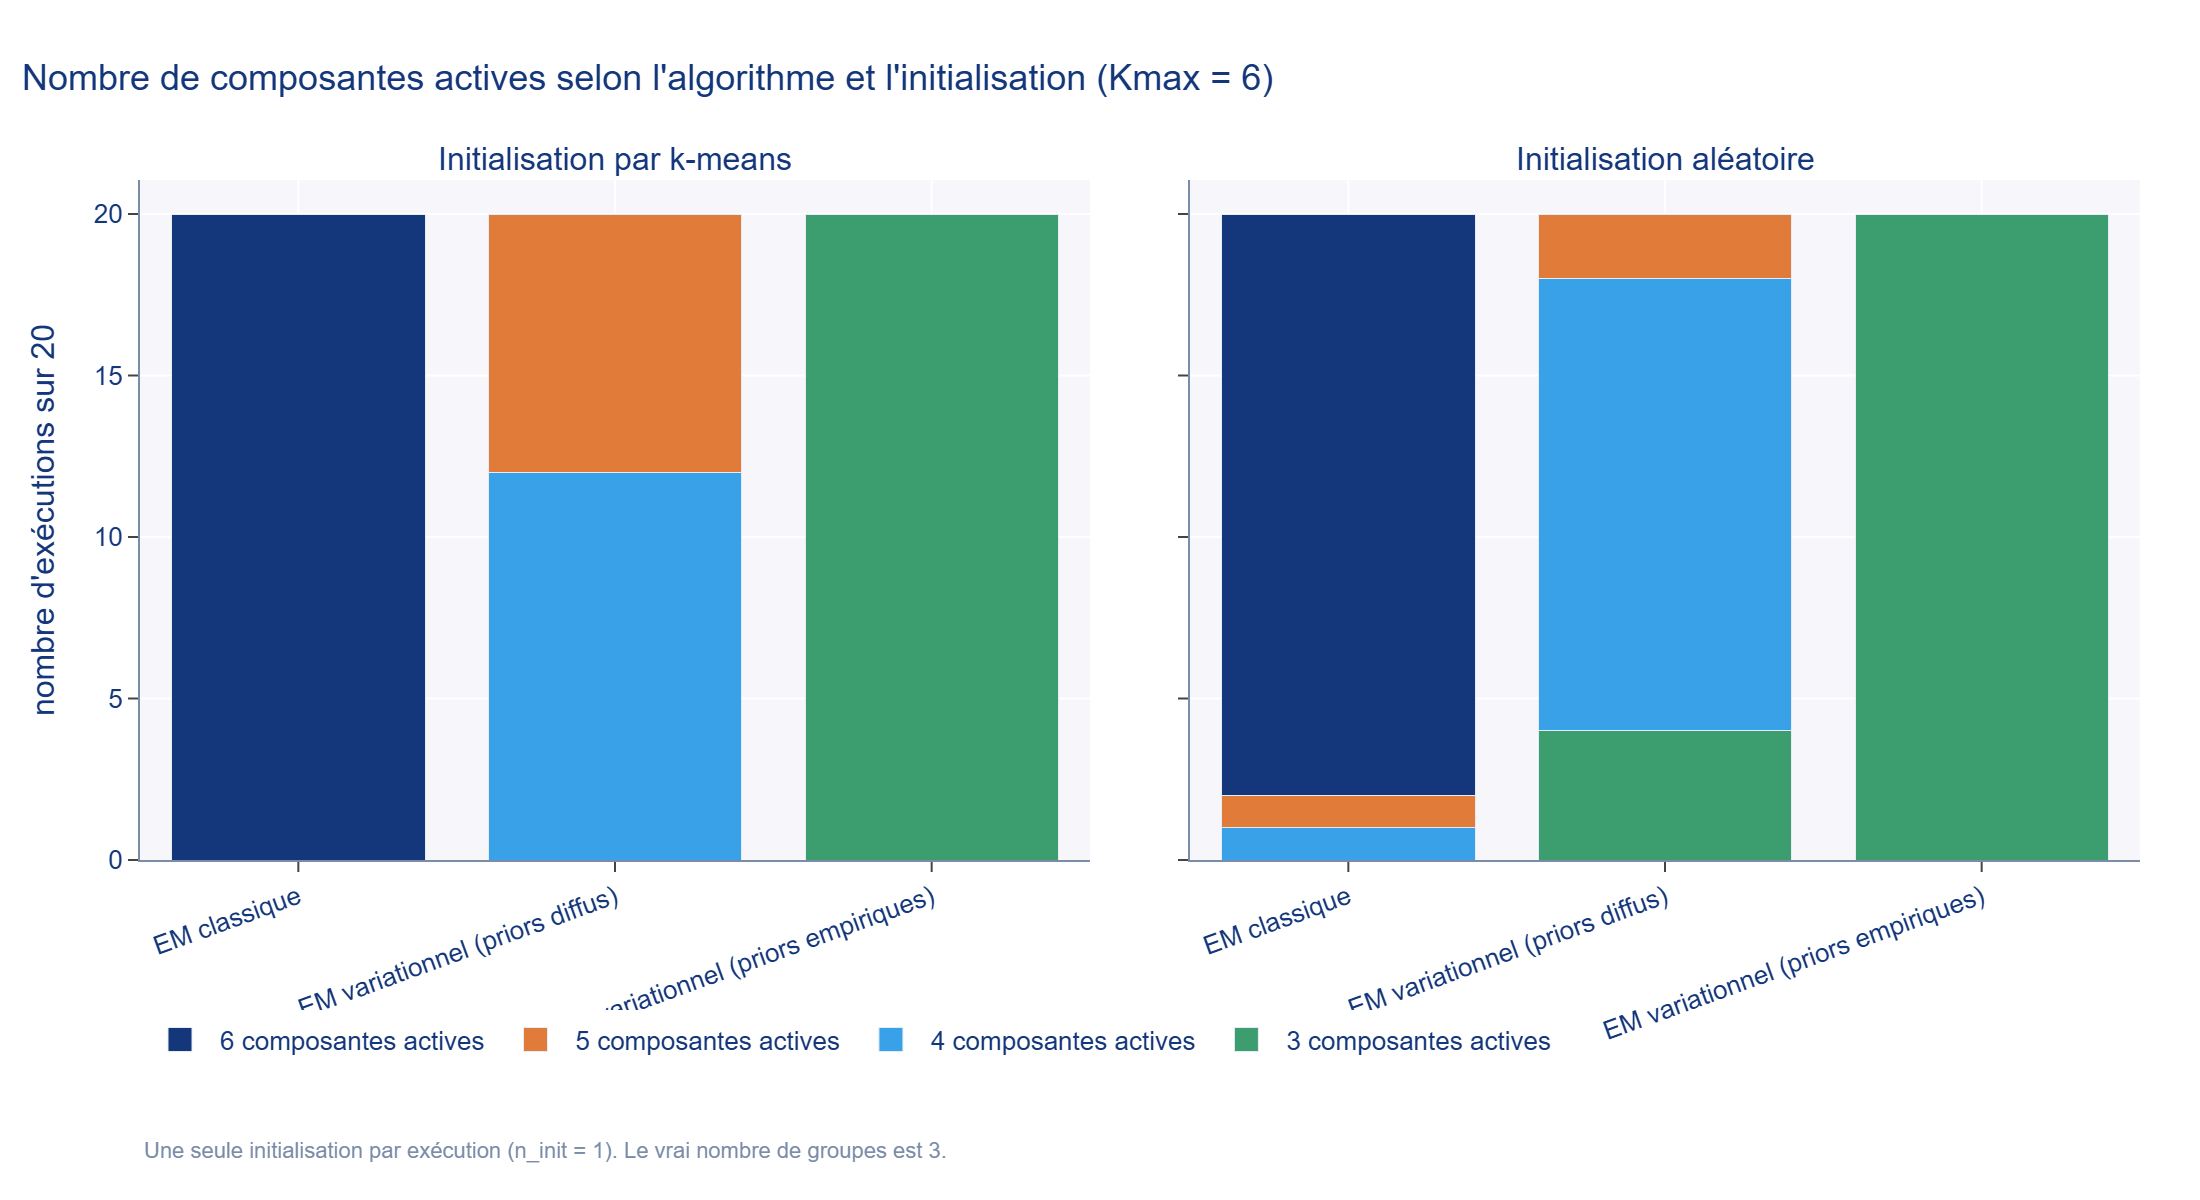
\includegraphics[width=0.95\textwidth]{figures/fig09.png}
\caption{Répartition du nombre de composantes actives selon l'algorithme et la stratégie d'initialisation (20 exécutions chacune, une initialisation par exécution).}
\label{fig:2_8}
\end{figure}
Avec les priors empiriques, l'EM variationnel retrouve exactement trois composantes actives dans 20 exécutions sur 20, quelle que soit la stratégie d'initialisation. Avec les priors diffus, le résultat est nettement plus sensible à l'initialisation : trois composantes seulement dans 4 exécutions sur 20 avec l'initialisation aléatoire, aucune avec k-means, les autres exécutions conservant quatre ou cinq composantes (une composante supplémentaire de faible poids n'étant pas complètement éliminée). L'EM classique conserve ses six composantes dans 20 exécutions sur 20 avec k-means et dans 18 sur 20 avec l'initialisation aléatoire ; dans les deux exécutions restantes, une composante s'effondre ($N_{k} < 1$), ce qui est un accident d'optimisation et non une sélection de modèle. La log-vraisemblance finale de l'EM classique varie entre -953,29 et -948,43 (écart-type 1,55) avec k-means et entre -955,67 et -944,12 (écart-type 2,35) avec l'initialisation aléatoire, ce qui confirme sa sensibilité aux optima locaux (section 1.6.3.a) sans résoudre le problème de fond : à K fixé à 6, aucune initialisation ne permet à l'EM classique de reconnaître que trois composantes suffiraient. Le mécanisme d'élagage de l'EM variationnel est donc robuste à l'initialisation lorsque les priors sont adaptés à l'échelle des données, et fragile lorsqu'ils ne le sont pas.

\subsection{Sensibilité au type de covariance}
L'ensemble des expériences précédentes ont été conduites avec des matrices de covariance pleines (full), c'est-à-dire sans contrainte sur la forme des ellipses de covariance de chaque composante. En pratique, il est fréquent de contraindre cette forme, tant pour réduire le nombre de paramètres libres et le risque de surapprentissage que pour accélérer les calculs. Les quatre contraintes les plus courantes, par ordre décroissant de flexibilité, sont : full (une matrice pleine par composante), tied (une unique matrice pleine partagée par toutes les composantes), diag (une matrice diagonale par composante) et spherical (une variance scalaire par composante). Pour l'EM variationnel, les variantes tied, diag et spherical ne sont pas dérivées au chapitre 1 ; elles utilisent un prior de Wishart partagé (tied) ou des priors Gamma sur les précisions (diag, spherical), également conjugués. Le tableau 2.12 reproduit l'expérience de la section 2.3.4 pour chacune de ces contraintes.

\begin{table}[H]
\centering
\small
\setlength{\tabcolsep}{0.14cm}
\begin{tabular}{|p{3.54cm}|p{3.54cm}|p{3.54cm}|p{3.54cm}|}
\hline
\textbf{Type de covariance} & \textbf{ARI : EM classique} & \textbf{ARI : EM variationnel} & \textbf{Composantes actives (variationnel)} \\
\hline
full & 0,715 & 0,990 & 3 \\
\hline
tied & 0,685 & 1,000 & 3 \\
\hline
diag & 0,727 & 0,990 & 3 \\
\hline
spherical & 0,726 & 1,000 & 3 \\
\hline
\end{tabular}
\caption{Indice de Rand ajusté et nombre de composantes actives selon le type de covariance (K = 6 imposé)}
\label{tab:2_12}
\end{table}
\begin{figure}[H]
\centering
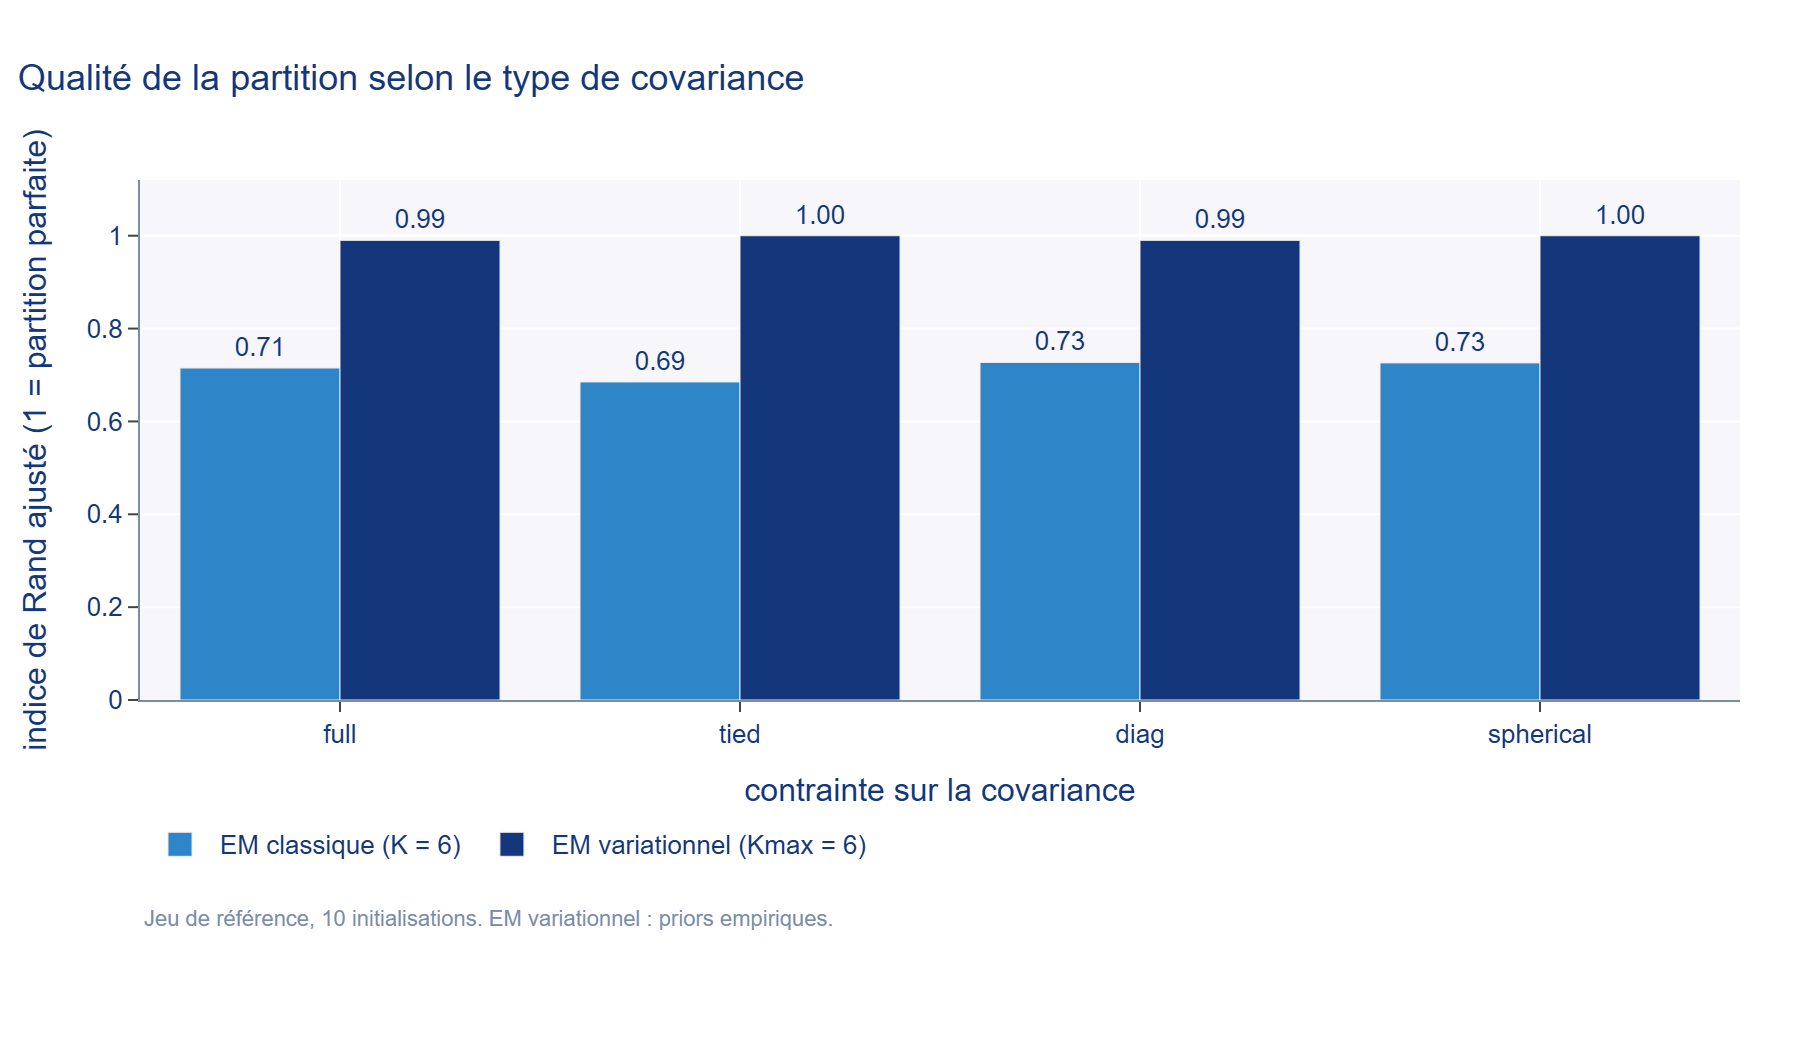
\includegraphics[width=0.85\textwidth]{figures/fig10.png}
\caption{Indice de Rand ajusté selon la contrainte imposée sur la covariance (K = 6 imposé).}
\label{fig:2_9}
\end{figure}
Ce résultat montre que le mécanisme d'élagage automatique de l'EM variationnel ne dépend pas de la forme de covariance retenue : dans les quatre cas, il identifie exactement les trois composantes attendues, avec un ARI compris entre 0,990 et 1,000. L'EM classique voit son ARI varier entre 0,685 et 0,727 selon la contrainte choisie, sans jamais atteindre la qualité de partition de l'EM variationnel. L'élagage n'est donc pas une particularité du cas des covariances pleines, mais une propriété du cadre bayésien variationnel, au moins pour les priors empiriques utilisés ici.

\subsection{Validation sur un jeu de données réel (Iris)}
L'ensemble des résultats précédents ont été obtenus sur un jeu synthétique, construit avec trois groupes gaussiens bien séparés. Afin de tester la robustesse des conclusions dans un cadre moins idéalisé, nous reproduisons l'expérience centrale de la section 2.3.1 sur le jeu de données Iris de Fisher (1936), qui comporte N = 150 observations en dimension D = 4 (longueur et largeur des pétales et des sépales), réparties en trois espèces réelles (Iris setosa, versicolor et virginica), avec K = 6 composantes imposées.

\begin{table}[H]
\centering
\small
\setlength{\tabcolsep}{0.14cm}
\begin{tabular}{|p{2.77cm}|p{4.2cm}|p{1.6cm}|p{1.9cm}|p{2.3cm}|}
\hline
\textbf{Algorithme} & \textbf{Poids de mélange (arrondis)} & \textbf{ARI} & \textbf{Silhouette} & \textbf{Composantes actives} \\
\hline
EM classique, K = 6 & 0,333 / 0,214 / 0,020 / 0,053 / 0,204 / 0,175 & 0,641 & 0,446 & 6 \\
\hline
EM variationnel, Kmax = 6 & 0,007 / 0,073 / 0,001 / 0,001 / 0,585 / 0,332 & 0,562 & 0,276 & 3 \\
\hline
EM classique, K = 3 & 0,333 / 0,364 / 0,303 & 0,904 & 0,501 & 3 \\
\hline
EM variationnel, Kmax = 3 & 0,190 / 0,333 / 0,476 & 0,684 & 0,400 & 3 \\
\hline
\end{tabular}
\caption{Résultats sur le jeu de données réel Iris (N = 150, D = 4)}
\label{tab:2_13}
\end{table}
\emph{Source : Iris de Fisher (1936), fichier UCI Machine Learning Repository ; calculs de l'auteur.}

\begin{figure}[H]
\centering
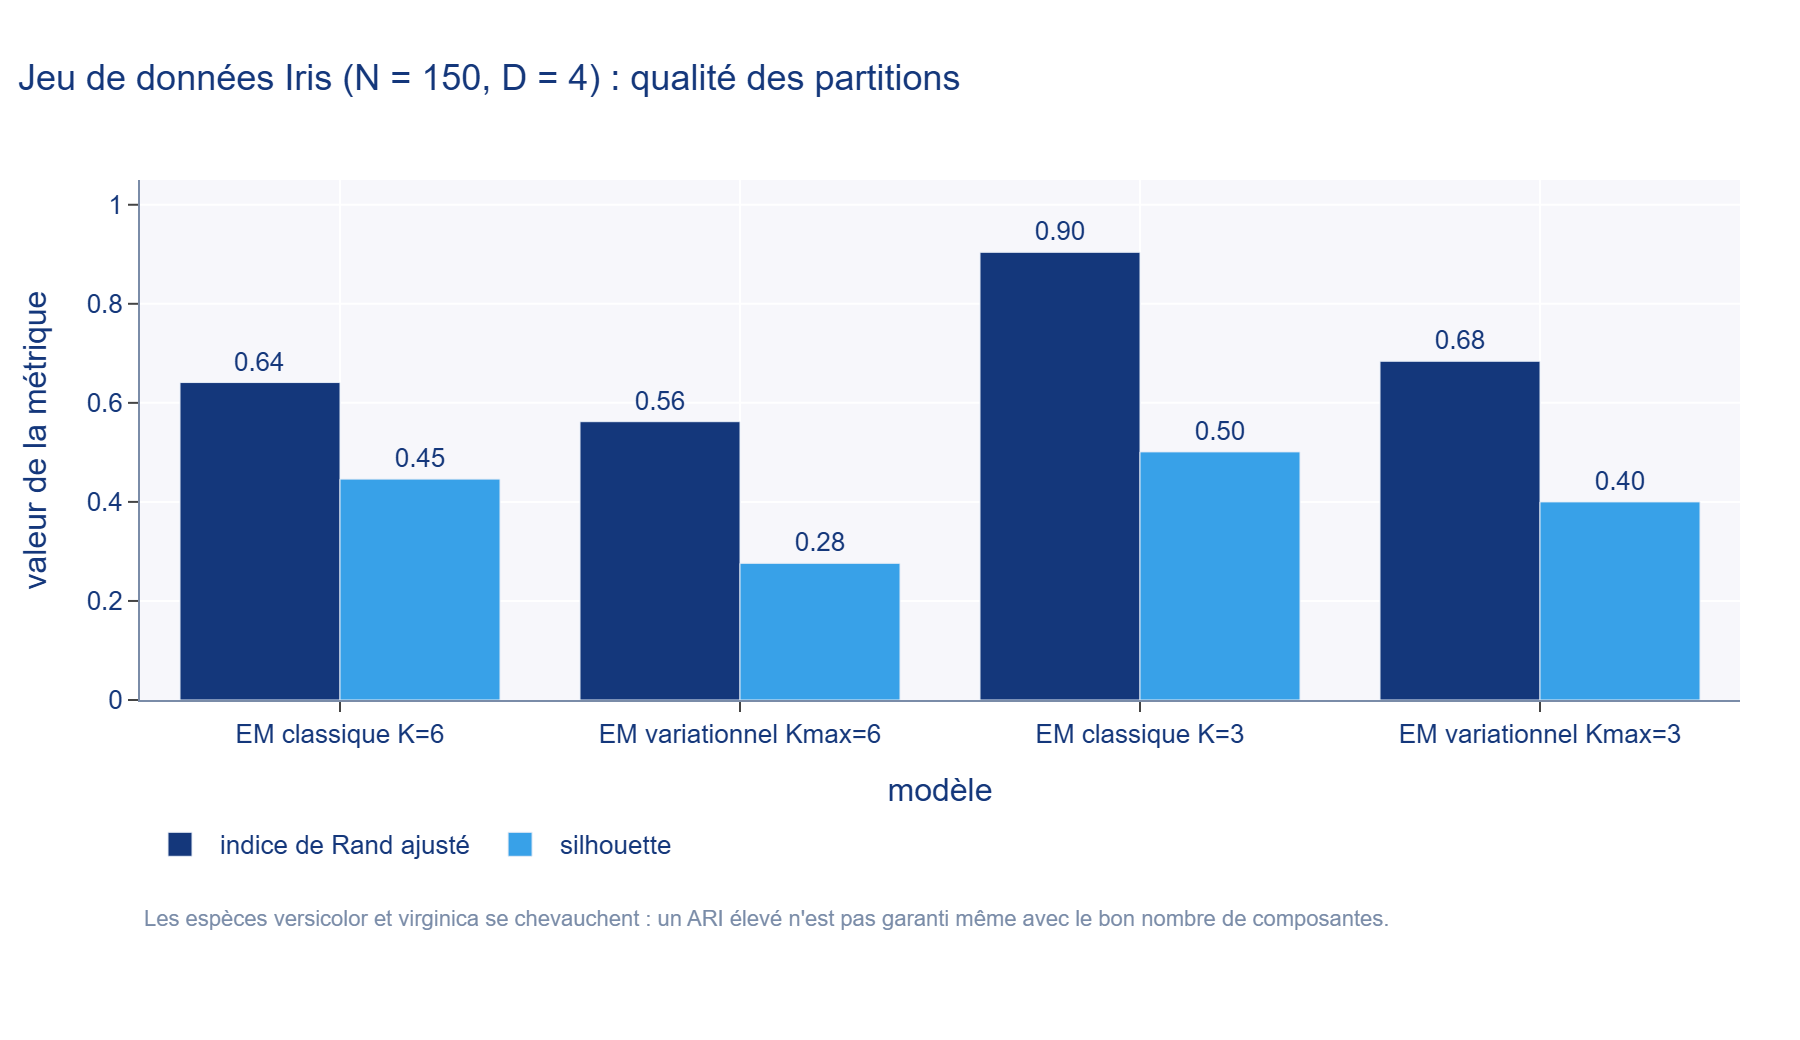
\includegraphics[width=0.85\textwidth]{figures/fig11.png}
\caption{Indice de Rand ajusté et silhouette sur le jeu Iris, selon l'algorithme et le nombre de composantes.}
\label{fig:2_10}
\end{figure}
Ce résultat, obtenu sur des données réelles, nuance la conclusion univoque de la section 2.3.4. À Kmax = 6, l'EM variationnel élague trois des six composantes mais son indice de Rand ajusté (0,562) est inférieur à celui de l'EM classique (0,641). Les poids finaux donnent la raison de cet écart : une composante de poids 0,585, proche de 2/3, regroupe les espèces versicolor et virginica, et une composante de poids 0,332, proche de 1/3, isole setosa. L'élagage fusionne donc les deux espèces qui se chevauchent, ce qui est cohérent avec le critère d'évidence puisque ces espèces ne forment pas deux nuages gaussiens séparés dans l'espace des quatre mesures, alors que les étiquettes de référence les distinguent. L'algorithme décide sur la base du support statistique observé dans les données, et non du nombre d'étiquettes disponibles : lorsque la structure réelle s'écarte de l'hypothèse d'un mélange de gaussiennes bien séparées, la solution de l'EM variationnel peut légitimement s'écarter du nombre d'étiquettes de référence, sans que cela constitue une défaillance de l'algorithme.

Avec Kmax = 3, l'EM variationnel obtient un ARI de 0,684, supérieur à celui de Kmax = 6 mais inférieur au 0,904 de l'EM classique à K = 3 exactement spécifié. Sur ce jeu réel, la meilleure stratégie reste donc, si l'on a une bonne raison de croire que K = 3 (ce que l'on sait ici grâce à la vérité terrain, mais qui ne serait pas connu en analyse exploratoire), d'utiliser l'EM classique avec ce K plutôt que de compter sur l'élagage pour le découvrir. Cette nuance, absente de l'étude synthétique, rappelle que la supériorité de l'EM variationnel, démontrée sur données synthétiques bien séparées, doit être relativisée sur des données réelles où les groupes ne sont pas des gaussiennes bien séparées.

\subsection{Sensibilité aux valeurs aberrantes}
Une dernière expérience examine le comportement des deux algorithmes en présence de valeurs aberrantes, situation fréquente en pratique et distincte de la simple surestimation de K. Dix points, tirés uniformément dans le carré $[-10 ; 15]^{2}$ (graine 7), ont été ajoutés au jeu de données de la section 2.3.1, puis les deux algorithmes ont été ajustés avec K = 6 sur ce jeu augmenté (N = 310).

\begin{table}[H]
\centering
\small
\setlength{\tabcolsep}{0.14cm}
\begin{tabular}{|p{4.84cm}|p{4.84cm}|p{4.84cm}|}
\hline
\textbf{Métrique} & \textbf{EM classique} & \textbf{EM variationnel} \\
\hline
ARI (calculé hors valeurs aberrantes) & 0,990 & 0,990 \\
\hline
Composantes actives & 6 & 5 \\
\hline
Trace maximale des covariances & 6,2 & 98,4 \\
\hline
Plus petit poids de mélange & 0,0065 & 0,0108 \\
\hline
\end{tabular}
\caption{Comportement des deux algorithmes en présence de 10 valeurs aberrantes ajoutées (N = 310, K = 6)}
\label{tab:2_14}
\end{table}
Les deux algorithmes retrouvent une partition quasi parfaite sur les points non aberrants (ARI de 0,990), ce qui montre qu'aucun n'est déstabilisé par un petit nombre de valeurs aberrantes dispersées. Les stratégies d'absorption diffèrent toutefois. L'EM classique répartit les valeurs aberrantes sur de petites composantes (poids minimal 0,0065) sans élargir aucune composante (trace maximale de 6,2). L'EM variationnel en absorbe plusieurs dans une composante diffuse, dont la trace de covariance (98,4) est environ seize fois supérieure, et conserve cinq composantes actives plutôt que trois. Ce comportement est compatible avec l'effet régularisant du prior Normal-Wishart, qui favorise l'élargissement d'une composante existante plutôt que la création de composantes quasi ponctuelles, mais cette expérience, fondée sur un seul tirage des valeurs aberrantes, ne permet pas de l'établir. Elle montre en revanche que la robustesse de l'EM variationnel n'est pas une insensibilité aux données aberrantes : le modèle conserve une composante supplémentaire non strictement nécessaire à la description du signal principal.

\subsection{Réplication sur des jeux de données indépendants}
Les sections précédentes reposent sur un jeu de données unique. Pour chiffrer l'incertitude des conclusions, le protocole de la section 2.3.1 (K = 6 imposé, dix initialisations par ajustement) a été répété sur R = 30 jeux de données indépendants, tirés avec les graines 1000 à 1029. Trois hypothèses, fixées avant l'analyse, sont testées : (H1) l'ARI moyen de l'EM variationnel dépasse celui de l'EM classique, ce que l'on décide si l'intervalle de confiance bootstrap à 95 \% de la différence appariée est strictement positif ; (H2) l'EM variationnel retrouve exactement trois composantes actives dans la majorité des jeux, ce que l'on décide si la borne basse de l'intervalle de Wilson à 95 \% dépasse 0,5 ; (H3) ces résultats dépendent du choix des priors. Les moyennes sont accompagnées d'intervalles de confiance bootstrap (5 000 rééchantillonnages) et les proportions d'intervalles de Wilson.

\begin{table}[H]
\centering
\small
\setlength{\tabcolsep}{0.1cm}
\begin{tabular}{|p{3.1cm}|p{2.6cm}|p{1.5cm}|p{2.9cm}|p{1.5cm}|p{1.5cm}|}
\hline
\textbf{Algorithme} & \textbf{ARI moyen [IC 95 \%]} & \textbf{Silhouette moyenne} & \textbf{Part de jeux à 3 composantes actives [IC 95 \%]} & \textbf{Itérations moyennes} & \textbf{Temps moyen (s)} \\
\hline
EM classique & 0,693 [0,677 ; 0,709] & 0,456 & 0 \% [0 ; 11 \%] (0 sur 30) & 9,2 & 0,21 \\
\hline
EM variationnel, priors diffus & 0,971 [0,953 ; 0,988] & 0,709 & 73 \% [56 ; 86 \%] (22 sur 30) & 118,8 & 4,04 \\
\hline
EM variationnel, priors empiriques & 0,999 [0,998 ; 1,000] & 0,746 & 100 \% [89 ; 100 \%] (30 sur 30) & 25,8 & 0,98 \\
\hline
\end{tabular}
\caption{Résultats moyens sur 30 jeux de données indépendants (K = 6 imposé)}
\label{tab:2_15}
\end{table}
\begin{table}[H]
\centering
\small
\setlength{\tabcolsep}{0.14cm}
\begin{tabular}{|p{6.0cm}|p{2.6cm}|p{2.6cm}|p{2.6cm}|}
\hline
\textbf{Comparaison (même jeu de données)} & \textbf{Différence moyenne d'ARI} & \textbf{IC 95 \% (bootstrap)} & \textbf{Jeux favorables à l'EM variationnel} \\
\hline
EM variationnel, priors diffus, moins EM classique & +0,278 & [0,258 ; 0,298] & 30 sur 30 \\
\hline
EM variationnel, priors empiriques, moins EM classique & +0,307 & [0,290 ; 0,322] & 30 sur 30 \\
\hline
\end{tabular}
\caption{Différences appariées d'indice de Rand ajusté entre EM variationnel et EM classique}
\label{tab:2_16}
\end{table}
\begin{figure}[H]
\centering
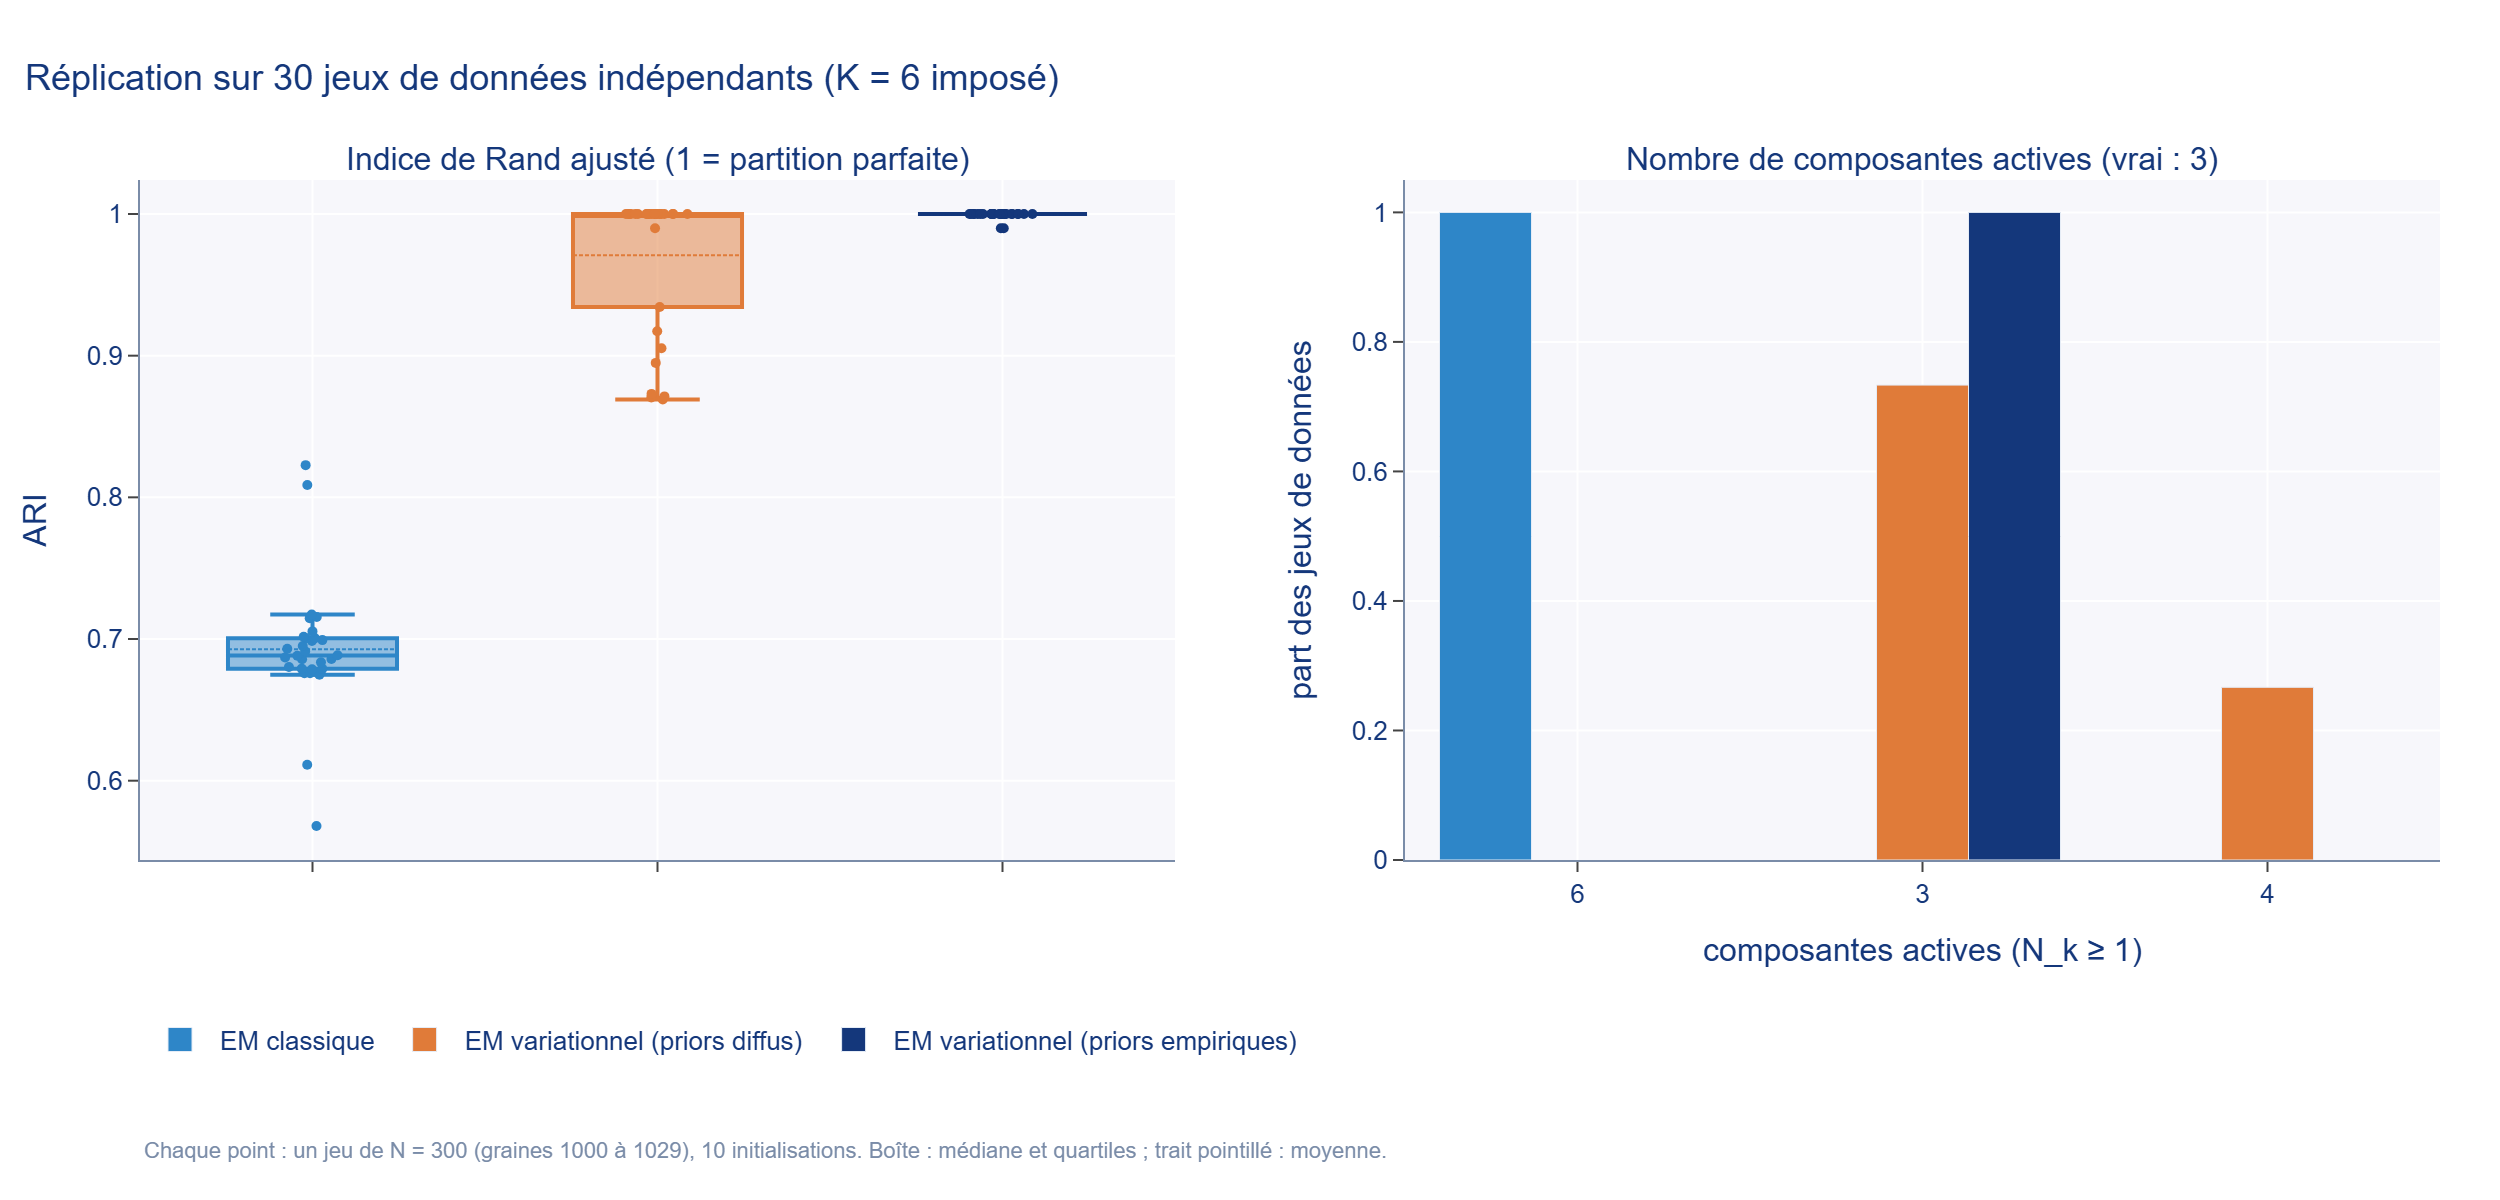
\includegraphics[width=0.95\textwidth]{figures/fig12.png}
\caption{Distribution de l'indice de Rand ajusté (à gauche, un point par jeu de données) et du nombre de composantes actives (à droite) sur 30 jeux de données indépendants.}
\label{fig:2_11}
\end{figure}
H1 est soutenue pour les deux jeux de priors : l'EM variationnel obtient un ARI supérieur à celui de l'EM classique sur chacun des 30 jeux, avec une différence moyenne de +0,28 (priors diffus) à +0,31 (priors empiriques) et des intervalles de confiance éloignés de zéro. H2 est soutenue pour les deux jeux de priors, mais avec des marges très différentes : 100 \% des jeux (borne basse de Wilson 89 \%) avec les priors empiriques, 73 \% (borne basse 56 \%) avec les priors diffus. H3 est confirmée : le choix des priors modifie l'ARI moyen (0,971 contre 0,999), le nombre d'itérations (119 contre 26) et le temps de calcul (4,0 s contre 1,0 s). L'EM classique, lui, ne retrouve jamais trois composantes (0 sur 30) puisqu'il conserve par construction les six composantes imposées. La variabilité entre jeux est faible pour les priors empiriques (écart-type de l'ARI de 0,003) et plus élevée pour les priors diffus (0,050), ce qui rejoint le constat de la section 2.3.9.

\section{Analyse des résultats et synthèse}
L'étude expérimentale conduite dans ce chapitre confirme, sur un exemple concret et reproductible, l'ensemble des différences théoriques et algorithmiques mises en évidence précédemment. Lorsque le nombre de composantes est correctement spécifié, les deux algorithmes produisent des résultats de qualité comparable, l'EM classique bénéficiant alors d'un net avantage en termes de rapidité d'exécution. En revanche, dès lors que le nombre de composantes est surestimé  situation extrêmement fréquente en pratique, où le nombre réel de groupes sous-jacents est rarement connu avec certitude , l'EM variationnel démontre un avantage net et reproductible sur trente jeux de données (section 2.3.13) grâce à son mécanisme d'élagage automatique, sous réserve d'un choix de priors adapté à l'échelle des données, produisant une partition à la fois plus parcimonieuse et plus fidèle à la structure réelle des données, sans qu'il soit nécessaire de relancer l'algorithme pour plusieurs valeurs de K ni de recourir à des critères de sélection externes tels que le BIC ou l'AIC.

Le tableau 2.17 propose une synthèse globale, intégrant l'ensemble des dimensions de comparaison abordées dans ce chapitre, et servira de référence pour la discussion des applications pratiques menée au chapitre 3.

\begin{table}[H]
\centering
\small
\setlength{\tabcolsep}{0.14cm}
\begin{tabular}{|p{4.84cm}|p{4.84cm}|p{4.84cm}|}
\hline
\textbf{Critère} & \textbf{EM classique} & \textbf{EM variationnel} \\
\hline
Simplicité conceptuelle & Élevée & Modérée \\
\hline
Coût computationnel & Faible & Modéré à élevé \\
\hline
Nécessité de fixer K a priori & Oui & Non (Kmax suffit) \\
\hline
Robustesse aux singularités & Faible (sans régularisation) & Élevée (régularisation par le prior) \\
\hline
Quantification de l'incertitude & Absente en natif & Native \\
\hline
Qualité sur données bien spécifiées & Très bonne & Très bonne \\
\hline
Qualité si K surestimé & Dégradée (sur-segmentation) & Robuste (élagage automatique) \\
\hline
Recommandation d'usage & K connu, prototypage rapide, grandes données simples & K incertain, besoin d'incertitude, données bruitées \\
\hline
\end{tabular}
\caption{Synthèse comparative globale entre l'EM classique et l'EM variationnel}
\label{tab:2_15}
\end{table}
Cette synthèse met en évidence que le choix entre les deux algorithmes ne doit pas être envisagé comme un choix entre une méthode « meilleure » et une méthode « moins bonne » dans l'absolu, mais comme un arbitrage dépendant du contexte applicatif  arbitrage que le chapitre 3 explore plus en détail à travers plusieurs domaines d'application concrets.

\section{Discussion critique du protocole expérimental}
Par honnêteté scientifique, il convient de discuter explicitement les limites du protocole expérimental suivi dans ce chapitre, avant d'en tirer des conclusions générales. Premièrement, la majorité des expériences (sections 2.3.1 à 2.3.10 et 2.3.12) reposent sur un unique jeu de données synthétique, construit par assemblage de trois gaussiennes isotropes bien séparées. Ce choix méthodologique, motivé par la volonté de disposer d'une vérité terrain non ambiguë pour calculer l'indice de Rand ajusté, favorise par construction le scénario le plus propice à l'EM variationnel : des groupes qui sont effectivement des gaussiennes, bien séparées, et de tailles comparables. La section 2.3.11, en introduisant le jeu de données réel Iris, a précisément eu pour objet de vérifier dans quelle mesure les conclusions tirées du cas synthétique se généralisent à un contexte moins favorable, et a montré que ce n'est pas systématiquement le cas : lorsque les groupes réels se chevauchent ou s'écartent de la forme gaussienne, l'avantage de l'EM variationnel peut s'atténuer, voire s'inverser localement.

Deuxièmement, les expériences des sections 2.3.1 à 2.3.12 reposent sur une seule graine de génération des données (graine 42). La section 2.3.13 lève en partie cette limite en répétant le protocole de la section 2.3.1 sur trente jeux indépendants, avec intervalles de confiance ; les autres expériences (Iris, valeurs aberrantes, type de covariance, scalabilité) n'ont pas été répliquées de cette manière, et la mesure des temps de calcul reste propre à une machine et à une implémentation.

Troisièmement, les dimensions considérées dans ce chapitre restent modestes (D = 2 pour la majorité des expériences, D = 4 pour Iris, D allant jusqu'à 20 pour l'étude de scalabilité de la section 2.3.6). Les grandes dimensions, fréquentes dans les applications réelles évoquées au chapitre 3 (bio-informatique, traitement d'image), posent des défis supplémentaires  malédiction de la dimensionnalité, estimation de matrices de covariance de grande taille à partir d'un nombre limité d'observations  qui n'ont pas été explorés empiriquement ici, au-delà des mesures de temps de calcul de la section 2.3.6. Ces trois limites, prises ensemble, invitent à interpréter les résultats de ce chapitre comme une démonstration rigoureuse et reproductible du mécanisme théorique décrit au chapitre 1, plutôt que comme une garantie de supériorité universelle de l'EM variationnel sur l'EM classique dans toutes les configurations de données possibles  nuance que le guide de décision pratique proposé à la section 3.5 s'efforce de refléter fidèlement.

Une quatrième limite, de nature plus méthodologique, mérite également d'être signalée : l'ensemble des métriques externes utilisées dans ce chapitre (ARI, score de silhouette) supposent implicitement l'existence d'une partition de référence contre laquelle comparer les résultats des algorithmes, ce qui n'est vrai que pour les données synthétiques et pour Iris, dont les étiquettes d'espèces sont connues indépendamment des variables mesurées. Dans la grande majorité des applications réelles évoquées au chapitre 3, en particulier en bio-informatique et en traitement du langage naturel, une telle vérité terrain n'existe tout simplement pas  la détermination du nombre « correct » de sous-populations cellulaires ou de thématiques textuelles étant précisément l'objet de l'analyse plutôt qu'une donnée préalable. Dans ces contextes d'analyse non supervisée pure, l'évaluation de la qualité d'un modèle de mélange doit nécessairement s'appuyer sur des critères internes  l'ELBO lui-même pour l'EM variationnel (section 1.7.6), ou les critères BIC/AIC pour l'EM classique (section 2.2.3) , dont ce chapitre a montré, à la section 2.3.3, qu'ils ne sont pas directement comparables en échelle absolue entre les deux algorithmes, ce qui limite d'autant la possibilité de trancher objectivement, en l'absence de vérité terrain, lequel des deux modèles offre le meilleur ajustement aux données.


%% ==== CHAPITRE : APPLICATIONS ET IMPLÉMENTATION ====
\chapter{APPLICATIONS ET IMPLÉMENTATION}
Les deux chapitres précédents ont établi les fondements théoriques de l'EM classique et de l'EM variationnel, puis confronté ces deux algorithmes sur un cas d'étude synthétique. Ce troisième et dernier chapitre s'attache à replacer ces algorithmes dans leur contexte applicatif réel, en explorant plusieurs domaines dans lesquels ils sont couramment employés, avant de présenter une implémentation complète en langage Python, accompagnée d'une analyse détaillée des résultats expérimentaux obtenus.

\section{Applications pratiques}
Les modèles à variables latentes ajustés par EM, sous sa forme classique ou variationnelle, trouvent des applications dans un très grand nombre de domaines. Cette section présente cinq domaines représentatifs, choisis pour la diversité des contraintes qu'ils imposent sur le choix entre EM classique et EM variationnel.

Le fil conducteur de cette revue applicative est le même que celui qui a guidé l'ensemble de ce mémoire : montrer que le choix entre EM classique et EM variationnel n'est jamais un choix purement académique, mais résulte d'un arbitrage concret entre plusieurs contraintes opérationnelles  le temps de calcul disponible, la confiance dont on dispose quant au nombre réel de composantes ou d'états sous-jacents, la nécessité ou non de quantifier l'incertitude pour la prise de décision en aval, et la robustesse requise face à des données potentiellement bruitées ou incomplètes. Les cinq domaines retenus ci-après  traitement du langage naturel, vision par ordinateur, bio-informatique, finance et systèmes de recommandation  ont été choisis précisément parce qu'ils illustrent, chacun à sa manière, une combinaison différente de ces contraintes, offrant ainsi un aperçu représentatif de la diversité des contextes dans lesquels l'algorithme EM, sous l'une ou l'autre de ses deux formes, continue d'être employé aujourd'hui, plus de cinquante ans après sa formalisation initiale.

\subsection{Traitement automatique du langage naturel}
En traitement automatique du langage naturel, le modèle d'allocation de Dirichlet latente (LDA), introduit par Blei, Ng et Jordan (2003), utilise une forme d'EM variationnel pour découvrir automatiquement les thématiques latentes d'un corpus de documents. Chaque document y est représenté comme un mélange de topics, et chaque topic comme une distribution sur le vocabulaire. Formellement, chaque document d est généré selon le processus suivant : on tire d'abord une distribution de topics $\theta d$ $\sim $ Dir($\alpha $), puis, pour chaque mot du document, on tire un topic zdn $\sim $ Catégorielle($\theta d$), et enfin un mot wdn $\sim $ Catégorielle($\beta zdn$), où $\beta k$ désigne la distribution sur le vocabulaire associée au topic k. La vraisemblance marginale d'un document,

\begin{equation}
\begin{adjustbox}{max width=0.92\linewidth}$\displaystyle p(w | \alpha {,} \beta ) = \int  p(\theta  | \alpha ) [\prod _{n} \Sigma _{z} p(z | \theta ) p(w_{n} | z{,} \beta )] d\theta $\end{adjustbox}
\tag{3.1}
\label{eq:3_1}
\end{equation}
est intractable pour la même raison que la vraisemblance marginale du GMM à la section 1.2.1 : elle fait intervenir une intégrale sur $\theta $ combinée à une somme sur les topics latents z. Blei, Ng et Jordan (2003) résolvent ce problème par une approche variationnelle en champ moyen tout à fait analogue à celle décrite au chapitre 1 pour le GMM bayésien, avec une distribution variationnelle factorisée q($\theta $, z) = q($\theta $ | $\gamma $) $\prod _{n}$ q($z_{n}$ | $\phi _{n}$), où q($\theta $ | $\gamma $) est une distribution de Dirichlet et q($z_{n}$ | $\phi _{n}$) une distribution catégorielle  soit exactement la même famille de distributions conjuguées (Dirichlet et catégorielle) que celle rencontrée à la section 1.7.3 pour les poids de mélange du GMM. Le nombre de topics devant être choisi a priori dans la version originale du modèle, les extensions bayésiennes non paramétriques de LDA, fondées sur des processus de Dirichlet hiérarchiques, exploitent précisément le mécanisme d'élagage automatique décrit à la section 1.7.4 pour déterminer le nombre de thématiques directement à partir des données.

\textbf{Correspondance formelle avec le champ moyen du GMM. }Il est instructif de mettre en regard, terme à terme, les mises à jour variationnelles de LDA et celles du GMM bayésien détaillées à la section 1.7.3.d, tant leur parenté structurelle est étroite. La mise à jour du paramètre variationnel $\phi _{nk}$ (probabilité variationnelle que le n-ième mot du document appartienne au topic k) s'écrit :

\begin{equation}
\begin{adjustbox}{max width=0.92\linewidth}$\displaystyle \phi _{nk} \propto  \exp [\mathbb{E}_{q}[\log  \theta _{k}] + \log  \beta _{k}{,}w_{n}]$\end{adjustbox}
\tag{3.2}
\label{eq:3_2}
\end{equation}
Cette formule est l'exact analogue, pour LDA, de la mise à jour des responsabilités $r_{ik}$ du GMM à l'équation (1.15) : le terme $\mathbb{E}$\_q[log $\theta _{k}$] y joue le rôle de $\mathbb{E}$[log $\pi _{k}$] (calculé, comme à la section 1.7.3.e, via la fonction digamma appliquée aux paramètres variationnels de Dirichlet $\gamma $), tandis que log $\beta _{k}$,$w_{n}$  la log-probabilité du mot observé sous le topic k  joue le rôle de la log-vraisemblance gaussienne log $\mathcal{N}$($x_{i}$|$\mu _{k}$,$\Sigma _{k}$) dans le GMM. La mise à jour du paramètre variationnel $\gamma $, quant à elle, s'écrit $\gamma _{k}$ = $\alpha $ + $\Sigma _{n}$ $\phi _{nk}$, formule en tout point analogue à la mise à jour $\alpha _{k}$ = $\alpha _{0}$ + $N_{k}$ du GMM bayésien (section 1.7.3.d), le terme $\Sigma _{n}$ $\phi _{nk}$ jouant ici le rôle du nombre effectif de points assignés $N_{k}$ = $\Sigma _{i}$ $r_{ik}$. Cette correspondance systématique, terme à terme, entre les deux modèles n'est pas fortuite : elle illustre concrètement l'affirmation faite à plusieurs reprises dans ce mémoire (notamment à la section 1.7.3.c) selon laquelle la formule générale du champ moyen variationnel, une fois appliquée à un choix de distributions conjuguées, produit mécaniquement des mises à jour de forme identique, quelle que soit la nature précise du modèle  mélange gaussien ou modèle de sujets textuels.

\subsubsection{Illustration : extraction de topics sur un corpus jouet}
Afin d'illustrer ce mécanisme, nous avons implémenté l'algorithme de Blei, Ng et Jordan (2003) à partir des équations (3.1) et (3.2) : pour chaque document, une itération à point fixe sur les paramètres variationnels $\phi $ et $\gamma $, puis, à l'étape M, la mise à jour $\beta _{kv} \propto \sum _{d} n_{dv}\,\phi _{dvk}$, où $n_{dv}$ est le nombre d'occurrences du mot v dans le document d. La borne variationnelle $\mathcal{L}(\gamma ,\phi ;\alpha ,\beta )$ est calculée à chaque itération. Le corpus jouet comprend douze phrases courtes en français réparties entre trois thématiques (animaux domestiques, finance, football). La table document-mot est construite avec pandas (mots d'au moins deux caractères, hors mots vides), avec trois topics, $\alpha $ = 0,1 et dix initialisations dont la meilleure borne est retenue.

\begin{lstlisting}[language=Python]
comptes = matrice_comptes(CORPUS)               # table document x mot (pandas)
C = torch.tensor(comptes.values, dtype=torch.float64)
res = lda_variationnel(C, K=3, alpha=0.1, graine=graine)
theta = res["theta"]                            # distribution de topics de chaque document
beta = res["beta"]                              # distribution sur le vocabulaire de chaque topic
\end{lstlisting}
\begin{center}\small\emph{Extrait de code : extraction de topics par LDA variationnel (code complet en annexe A)}\end{center}
La borne variationnelle croît à chaque itération, ce qui valide l'implémentation de l'éq. (3.2), et l'algorithme converge en 4 itérations (meilleure borne : -131,63). Les trois topics obtenus sont donnés au tableau~
ef{tab:3_1b}.

\begin{table}[H]
\centering
\small
\setlength{\tabcolsep}{0.14cm}
\begin{tabular}{|p{2.5cm}|p{12.3cm}|}
\hline
\textbf{Topic} & \textbf{Six mots les plus probables} \\
\hline
0 & football, reprend, end, remporte, week, equipe \\
\hline
1 & taux, but, joueur, rencontre, decisif, marque \\
\hline
2 & chat, chien, actions, progressent, marche, financier \\
\hline
\end{tabular}
\caption{Topics extraits par LDA variationnel sur le corpus jouet (trois topics demandés)}
\label{tab:3_1b}
\end{table}
Seul le topic 0 est sémantiquement cohérent (football). Le topic 1 mélange un terme financier (taux) et des termes sportifs, le topic 2 mélange les animaux domestiques et un vocabulaire financier. En prenant, pour chaque document, le topic dominant, 8 documents sur 12 sont rattachés au topic qui correspond à leur thème (pureté de 0,67 ; distributions complètes à l'annexe A.4). Ce résultat décevant est attendu : avec douze documents et un vocabulaire de quelques dizaines de mots, l'estimation des distributions $\beta _{k}$ est très imprécise, et la solution dépend de l'initialisation. Il ne faut donc pas interpréter les topics eux-mêmes ; la croissance de la borne variationnelle valide l'algorithme, pas la qualité thématique sur un corpus aussi petit. Les modèles de mélange gaussien sont par ailleurs couramment utilisés pour le regroupement de plongements lexicaux, où l'incertitude sur l'appartenance à un cluster sémantique est souvent aussi informative que l'appartenance elle-même, ce qui plaide en faveur de l'EM variationnel dans ce contexte.

\subsection{Vision par ordinateur}
En vision par ordinateur, les GMM sont largement employés pour la segmentation d'images, où chaque pixel  ou chaque région issue d'une sur-segmentation préalable  est modélisé comme provenant d'une composante gaussienne dans l'espace des couleurs (par exemple l'espace RGB ou l'espace teinte-saturation-luminosité) ou des descripteurs de texture. La segmentation revient alors à résoudre un problème de mélange gaussien en dimension D = 3 (couleur) ou plus (texture), tout à fait analogue à celui étudié au chapitre 2, à ceci près que N désigne ici le nombre de pixels de l'image, qui peut atteindre plusieurs millions pour des images haute résolution  ce qui replace directement la question de la scalabilité computationnelle, étudiée à la section 2.3.6, au cœur de la décision entre EM classique et EM variationnel pour cette application.

Dans l'algorithme classique de soustraction de fond par mélange de gaussiennes (Stauffer et Grimson, 1999), chaque pixel de coordonnées (u, v) est modélisé indépendamment par son propre petit GMM à 3-5 composantes sur la séquence temporelle de ses valeurs de couleur, mis à jour de façon incrémentale à chaque nouvelle image par une variante de l'EM online (section 1.6.6) : Pour une nouvelle observation de couleur $x_{t}$(u,v), on met à jour les poids par $\hat{\pi }$$_{k}$ ← (1-$\rho $) $\pi _{k}$ + $\rho $ $M_{k}$,$_{t}$, où $M_{k}$,$_{t}$ = 1 si $x_{t}$ correspond à la composante k (au sens d'un test de distance de Mahalanobis à quelques écarts-types) et 0 sinon, et $\rho $ est un taux d'apprentissage fixé. Les composantes de poids $\pi _{k}$ les plus élevés et de variance la plus faible sont alors classées comme « fond » (arrière-plan statique), les autres comme « premier plan » (objets en mouvement)  une règle de décision directement héritée de l'interprétation des poids de mélange comme fréquences relatives d'occurrence, établie à la section 1.6.2.c.

\subsection{Bio-informatique}
En bio-informatique, les modèles de mélange sont utilisés pour l'analyse de données d'expression génique, où l'on cherche à identifier des sous-populations de cellules ou de gènes co-régulés à partir de données de séquençage à cellule unique (single-cell RNA-seq). Ces données présentent typiquement plusieurs milliers de dimensions (une par gène mesuré) pour un nombre de cellules pouvant atteindre plusieurs centaines de milliers, ce qui pose, comme en vision par ordinateur, un problème de scalabilité aigu. Le nombre réel de sous-populations cellulaires étant rarement connu a priori  il constitue en réalité souvent l'objet même de l'étude biologique , et les données étant typiquement bruitées, l'EM variationnel, et plus particulièrement ses extensions à des priors hiérarchiques de type processus de Dirichlet (Rasmussen, 2000), y est largement préféré à l'EM classique, malgré son coût computationnel plus élevé identifié à la section 2.3.6, précisément parce que la sélection automatique du nombre de composantes constitue ici un enjeu scientifique de première importance, et non un simple raffinement technique.

Les modèles de Markov cachés, ajustés par l'algorithme de Baum-Welch  une instance de l'EM classique où l'étape E s'effectue au moyen des algorithmes forward-backward plutôt que par un simple calcul de responsabilités indépendantes, comme détaillé à la section 1.6.6 , demeurent quant à eux la méthode de référence pour l'annotation de séquences génomiques et la prédiction de structures secondaires de protéines, domaines où la structure séquentielle des données (la dépendance d'un état au précédent) prime sur la quantification fine de l'incertitude, et où la rapidité de l'EM classique permet de traiter des génomes entiers, comportant plusieurs milliards de paires de bases, dans des délais raisonnables. L'exemple numérique de prévision météorologique de la section 1.6.6 se transpose directement à ce contexte en remplaçant les deux états « Beau » et « Pluvieux » par des états biologiques tels que « région codante » et « région non codante » d'une séquence d'ADN, et les observations « Parapluie »/« Pas de parapluie » par les quatre nucléotides A, C, G, T.

\subsection{Finance}
En finance quantitative, les modèles de mélange gaussien sont employés pour la modélisation des rendements d'actifs financiers, dont la distribution empirique présente typiquement des queues plus épaisses (leptokurtiques) qu'une loi normale simple  phénomène qu'un mélange de deux à quatre régimes gaussiens, de variances différentes, permet de capturer de façon parcimonieuse, sans recourir à des familles de distributions plus complexes. Formellement, le rendement $r_{t}$ d'un actif à l'instant t est modélisé par $r_{t}$ | $z_{t}$=k $\sim $ $\mathcal{N}$($\mu _{k}$, $\sigma _{k}^{2}$), où l'état de régime $z_{t}$ (par exemple « calme », k=1, ou « turbulent », k=2) suit lui-même une chaîne de Markov cachée, exactement comme à la section 1.6.6  la seule différence avec l'exemple météorologique de cette section étant que les observations $r_{t}$ y sont continues (gaussiennes) plutôt que discrètes (parapluie/pas de parapluie), ce qui ne change rien à la structure de l'algorithme de Baum-Welch, seule la forme de la matrice d'émission B étant remplacée par une densité gaussienne $\mathcal{N}$($\mu _{k}$, $\sigma _{k}^{2}$).

Dans ce contexte, la quantification de l'incertitude offerte par l'EM variationnel présente un intérêt particulier pour la gestion des risques : disposer d'une distribution a posteriori sur les paramètres du modèle, plutôt que d'une simple estimation ponctuelle, permet de propager l'incertitude d'estimation jusque dans le calcul de mesures de risque telles que la valeur à risque (VaR) ou la perte attendue en cas de dépassement de seuil (Expected Shortfall), en intégrant ces mesures de risque sur la distribution a posteriori plutôt qu'en les calculant à partir d'une unique estimation ponctuelle des paramètres, ce qui produit des estimations de risque plus prudentes et mieux calibrées, en particulier lorsque l'historique de données disponible est de taille limitée. La détection de régimes de marché (haussier, baissier, volatil) au moyen de modèles de Markov cachés constitue également une application répandue, généralement traitée par l'EM classique en raison des contraintes de temps réel imposées par le trading algorithmique, où les paramètres du modèle doivent être réestimés à haute fréquence.

\subsection{Systèmes de recommandation}
Dans les systèmes de recommandation, les modèles à variables latentes sont au cœur des approches de filtrage collaboratif fondées sur la factorisation matricielle probabiliste, où les goûts d'un utilisateur u et les caractéristiques d'un article i sont représentés par des vecteurs latents $p_{u}$ et $q_{i}$, la note attendue étant modélisée par leur produit scalaire, $\hat{r}$$_{ui}$ $\approx $ $p_{u}^{T}q_{i}$. Le modèle bayésien complet place des priors gaussiens sur ces vecteurs latents, $p_{u}$ $\sim $ $\mathcal{N}$(0, $\lambda ^{-1}I$) et $q_{i}$ $\sim $ $\mathcal{N}$(0, $\lambda ^{-1}I$), et l'inférence variationnelle en champ moyen  appliquant exactement le même principe que celui détaillé à la section 1.7.3 pour le GMM, mais avec q(P, Q) = $\prod _{u}$ q($p_{u}$) $\prod _{i}$ q($q_{i}$) comme famille variationnelle plutôt que la factorisation en poids/moyennes/précisions du GMM  permet d'estimer conjointement les distributions a posteriori de tous les vecteurs latents à partir des seules notes effectivement observées, notoirement incomplètes dans ce contexte (un utilisateur ne note qu'une infime fraction du catalogue).

L'EM variationnel bayésien permet d'y intégrer naturellement l'incertitude liée à la faible quantité d'interactions disponibles pour les nouveaux utilisateurs ou les nouveaux articles  le problème dit du démarrage à froid , en exploitant la distribution a posteriori sur ($p_{u}$, $q_{i}$) pour proposer des recommandations qui tiennent compte explicitement de cette incertitude, par exemple à travers des stratégies d'exploration-exploitation de type échantillonnage de Thompson, où l'on tire aléatoirement un jeu de paramètres selon leur distribution a posteriori avant de recommander l'article de score maximal sous ce tirage, ce qui favorise naturellement l'exploration des articles pour lesquels l'incertitude  et donc le potentiel d'information à gagner  est la plus grande.

\begin{table}[H]
\centering
\small
\setlength{\tabcolsep}{0.14cm}
\begin{tabular}{|p{4.84cm}|p{4.84cm}|p{4.84cm}|}
\hline
\textbf{Domaine} & \textbf{Application type} & \textbf{Algorithme généralement préféré} \\
\hline
Traitement du langage naturel & Modélisation de topics (LDA), clustering sémantique & EM variationnel \\
\hline
Vision par ordinateur (temps réel) & Segmentation vidéo, soustraction de fond & EM classique \\
\hline
Vision par ordinateur (hors ligne) & Segmentation d'images médicales & EM variationnel \\
\hline
Bio-informatique & Sous-populations cellulaires, séquençage & EM variationnel \\
\hline
Bio-informatique & Annotation de séquences (HMM) & EM classique \\
\hline
Finance & Gestion des risques, VaR & EM variationnel \\
\hline
Finance & Détection de régimes (trading algorithmique) & EM classique \\
\hline
Systèmes de recommandation & Démarrage à froid, exploration-exploitation & EM variationnel \\
\hline
\end{tabular}
\caption{Synthèse des domaines d'application et de l'algorithme le plus adapté}
\label{tab:3_1}
\end{table}
\section{Implémentation de l'EM classique}
L'EM classique est implémenté en PyTorch à partir des équations du chapitre 1, sans bibliothèque de modélisation : seules les opérations élémentaires (algèbre linéaire, factorisation de Cholesky, fonction digamma) sont utilisées, et les critères d'évaluation (BIC, AIC, indice de Rand ajusté, silhouette) sont écrits explicitement. Le code complet figure à l'annexe A ; les extraits ci-dessous montrent la correspondance avec les équations.

\subsection{Étapes E et M}
La densité gaussienne est évaluée par la factorisation de Cholesky de la covariance (section 2.2.2), puis l'étape E calcule les responsabilités en log-espace avec l'astuce du log-sum-exp (équations 1.15 et 1.18). L'étape M applique les mises à jour de l'équation (1.16).

\begin{lstlisting}[language=Python]
def logsumexp_stable(a: Tensor, dim: int = 1, keepdim: bool = True) -> Tensor:
    """Équation (1.18) : log sum exp(a_k) = a_max + log sum exp(a_k - a_max)."""
    a_max = a.max(dim=dim, keepdim=True).values
    out = a_max + torch.log(torch.exp(a - a_max).sum(dim=dim, keepdim=True))
    return out if keepdim else out.squeeze(dim)

def log_gauss(X: Tensor, mu: Tensor, cov: Tensor) -> Tensor:
    """log N(x | mu, cov) pour toutes les lignes de X, via Cholesky (section 2.2.2)."""
    D = X.shape[1]
    L = torch.linalg.cholesky(cov)
    z = torch.linalg.solve_triangular(L, (X - mu).T, upper=False)
    logdet = 2.0 * torch.log(torch.diagonal(L)).sum()
    return -0.5 * (D * LOG2PI + logdet + (z ** 2).sum(dim=0))

def _etape_e(X, pi, mu, cov):
    """Étape E (1.15) en log-espace : retourne (r, log p(x_i | theta))."""
    K = len(pi)
    log_r = torch.stack([torch.log(pi[k] + 1e-300) + log_gauss(X, mu[k], cov[k])
                         for k in range(K)], dim=1)
    log_norm = logsumexp_stable(log_r, dim=1)
    return torch.exp(log_r - log_norm), log_norm.squeeze(1)

def _etape_m(X, r, cov_type, reg):
    """Étape M (1.16) : pi_k = N_k/N, mu_k = moyenne pondérée, Sigma_k = covariance pondérée."""
    N = X.shape[0]
    Nk = r.sum(0) + 1e-10
    pi = Nk / N
    mu = (r.T @ X) / Nk[:, None]
    cov = _covariances_em(X, r, mu, Nk, cov_type, reg)
    return pi, mu, cov
\end{lstlisting}
\begin{center}\small\emph{Extrait de code : étapes E et M de l'EM classique (équations 1.15, 1.16 et 1.18)}\end{center}

\subsection{Initialisation, relances et critère d'arrêt}
Deux initialisations sont disponibles : par k-means (avec initialisation k-means++), qui donne un point de départ proche de la solution, et aléatoire (K points de données tirés au hasard et covariance globale, section 1.6.2.a). L'algorithme est relancé n\_init fois et la solution de plus grande log-vraisemblance est conservée. L'arrêt a lieu lorsque la variation de la log-vraisemblance passe sous le seuil $\varepsilon $, soit par observation (convention du protocole du chapitre 2 pour l'EM classique), soit en valeur totale (équation de la section 1.6.2.a) selon l'option choisie.

\begin{lstlisting}[language=Python]
def _em_une_fois(X, K, cov_type, n_iter, tol, reg, init, graine, tol_par_obs):
    N, D = X.shape
    pi, mu, cov = _init_em(X, K, cov_type, init, graine, reg)
    hist, converge = [], False
    for it in range(n_iter):
        r, log_norm = _etape_e(X, pi, mu, cov)
        hist.append(float(log_norm.sum()))
        ecart = abs(hist[-1] - hist[-2]) / (N if tol_par_obs else 1.0) if it > 0 else float("inf")
        if ecart < tol:
            converge = True
            break
        pi, mu, cov = _etape_m(X, r, cov_type, reg)
    r, log_norm = _etape_e(X, pi, mu, cov)
    return {"pi": pi, "mu": mu, "cov": cov, "r": r, "loglik": float(log_norm.sum()),
            "ll_hist": hist, "n_iter": len(hist), "converge": converge}
\end{lstlisting}
\begin{center}\small\emph{Extrait de code : boucle de l'EM classique avec test d'arrêt}\end{center}

\section{Implémentation de l'EM variationnel}
L'EM variationnel pour le GMM bayésien est implémenté de la même façon. Les espérances nécessaires (équations 1.29 et 1.30) sont calculées avec la fonction digamma de PyTorch, les mises à jour suivent les équations (1.26) et (1.28), et l'ELBO de l'équation (1.31) est évaluée exactement à chaque itération (annexe B).

\subsection{Étapes E et M variationnelles}
\begin{lstlisting}[language=Python]
def _attendus(P, D):
    """E[ln|Lambda_k|] (1.29) et E[Lambda_k] pour chaque composante."""
    if P["cov_type"] in ("full", "tied"):
        i = torch.arange(1, D + 1, dtype=torch.float64)
        Elogdet = (torch.special.digamma((P["nu"][:, None] + 1 - i) / 2).sum(-1)
                   + D * LN2 + torch.logdet(P["W"]))
        Elam = P["nu"][:, None, None] * P["W"]
    else:
        psi = torch.special.digamma(P["a"]) - torch.log(P["b"])
        Elogdet = psi.sum(-1)
        Elam = torch.diag_embed(P["a"] / P["b"])
    return Elogdet, Elam

def _etape_e_var(X, P):
    """Étape E variationnelle, équation (1.27), avec la forme quadratique (1.30)."""
    N, D = X.shape
    Elogpi = torch.special.digamma(P["alpha"]) - torch.special.digamma(P["alpha"].sum())
    Elogdet, Elam = _attendus(P, D)
    diff = X[None, :, :] - P["m"][:, None, :]
    quad = D / P["beta"][None, :] + torch.einsum("knd,kde,kne->nk", diff, Elam, diff)
    log_rho = Elogpi[None] + 0.5 * Elogdet[None] - 0.5 * D * LOG2PI - 0.5 * quad
    log_norm = logsumexp_stable(log_rho, dim=1)
    return torch.exp(log_rho - log_norm), log_norm.squeeze(1)
\end{lstlisting}
\begin{center}\small\emph{Extrait de code : étape E variationnelle (équations 1.27, 1.29 et 1.30)}\end{center}
\begin{lstlisting}[language=Python]
def _etape_m_var(Nk, xbar, Sk, pr: PrioriNW, cov_type):
    """Étape M variationnelle, équations (1.26) et (1.28), plus les variantes de covariance."""
    K, D = xbar.shape
    beta = pr.beta0 + Nk
    m = (pr.beta0 * pr.m0 + Nk[:, None] * xbar) / beta[:, None]
    d0 = xbar - pr.m0
    terme_prior = (pr.beta0 * Nk / (pr.beta0 + Nk))
    sc = Nk[:, None, None] * Sk + terme_prior[:, None, None] * d0[:, :, None] * d0[:, None, :]
    P = {"alpha": pr.alpha0 + Nk, "beta": beta, "m": m, "cov_type": cov_type}
    if cov_type == "full":
        P["nu"] = pr.nu0 + Nk
        P["Winv"] = pr.W0inv[None] + sc
        P["W"] = torch.linalg.inv(P["Winv"])
    elif cov_type == "tied":
        P["nu"] = torch.full((K,), pr.nu0 + float(Nk.sum()))
        Winv = pr.W0inv + sc.sum(0)
        P["Winv"] = Winv.expand(K, D, D).clone()
        P["W"] = torch.linalg.inv(Winv).expand(K, D, D).clone()
    else:                                       # diag, spherical : priors Gamma sur les précisions
        a0 = pr.nu0 / 2.0
        b0 = 0.5 * torch.diagonal(pr.W0inv)
        sd = torch.diagonal(sc, dim1=1, dim2=2)
        if cov_type == "diag":
            P["a"] = (a0 + Nk / 2.0)[:, None].expand(K, D).clone()
            P["b"] = b0[None] + 0.5 * sd
        else:
            P["a"] = (a0 + D * Nk / 2.0)[:, None].expand(K, D).clone()
            P["b"] = (b0.mean() + 0.5 * sd.sum(1))[:, None].expand(K, D).clone()
    return P
\end{lstlisting}
\begin{center}\small\emph{Extrait de code : étape M variationnelle (équations 1.26 et 1.28 pour la covariance pleine)}\end{center}

Les variantes de covariance tied, diag et spherical, absentes du chapitre 1, sont obtenues avec un prior de Wishart partagé ou des priors Gamma sur les précisions.

\subsection{Effet de l'initialisation et des priors}
Le tableau~
ef{tab:3_2} compare, sur le jeu de données de référence (K = 6, graine 42), les stratégies d'initialisation et les deux jeux de priors de la section 2.3.1.

\begin{table}[H]
\centering
\small
\setlength{\tabcolsep}{0.1cm}
\begin{tabular}{|p{6.4cm}|p{1.8cm}|p{1.2cm}|p{1.8cm}|p{1.8cm}|}
\hline
\textbf{Configuration} & \textbf{Composantes actives} & \textbf{ARI} & \textbf{Silhouette} & \textbf{Itérations} \\
\hline
EM classique, init. k-means (10 relances) & 6 & 0,715 & 0,450 & 8 \\
\hline
EM classique, init. aléatoire (1 essai) & 6 & 0,834 & 0,382 & 44 \\
\hline
EM variationnel, priors empiriques, init. k-means & 3 & 0,990 & 0,739 & 25 \\
\hline
EM variationnel, priors diffus, init. k-means & 4 & 0,985 & 0,646 & 103 \\
\hline
EM variationnel, priors diffus, init. aléatoire (1 essai) & 4 & 0,884 & 0,589 & 200 (maximum) \\
\hline
\end{tabular}
\caption{Effet de l'initialisation et des priors (jeu de référence, K = 6)}
\label{tab:3_2}
\end{table}
Deux enseignements se dégagent. D'abord, l'initialisation aléatoire demande beaucoup plus d'itérations que k-means pour l'EM classique (44 contre 8) et empêche l'EM variationnel avec priors diffus de converger avant le maximum de 200 itérations : le mécanisme d'élagage met du temps à s'installer lorsque les priors sont mal calibrés. Ensuite, le résultat qualitatif (six composantes pour l'EM classique, trois ou quatre pour l'EM variationnel) est stable d'une configuration à l'autre, mais le nombre exact de composantes actives de l'EM variationnel dépend des priors, ce que la réplication de la section 2.3.13 quantifie.

\section{Résultats expérimentaux et discussion}
L'exécution du protocole du chapitre 2 avec ces implémentations donne les résultats détaillés dans ce chapitre : l'EM classique conserve ses six composantes (tableau 2.5), tandis que l'EM variationnel avec priors empiriques converge vers trois composantes dominantes de poids proches de 1/3, les trois autres voyant leur nombre effectif de points chuter à 0,3 (tableau 2.6). Du point de vue de l'écriture du code, le passage de l'EM classique à l'EM variationnel se limite à remplacer les mises à jour (1.15) et (1.16) par (1.26) à (1.30) et à ajouter les hyperparamètres des priors, alors que les propriétés statistiques des deux algorithmes diffèrent radicalement.

Il convient de nuancer cette conclusion par les limites identifiées à la section 1.7.9 : la sensibilité de l'EM variationnel au choix des hyperparamètres du prior est un point de vigilance (tableau~
ef{tab:3_2} et section 2.3.13), de même que le surcoût computationnel, qui peut devenir significatif sur des jeux de grande dimension ou de grande taille, situation dans laquelle les variantes stochastiques de la section 1.7.7 deviennent nécessaires. Elles ont été implémentées : sur le jeu de référence avec trois composantes, l'EM online et l'inférence variationnelle stochastique (mini-lots de 30 observations) retrouvent la partition (ARI de 1,00 et 0,99), l'EM stochastique visite des solutions de log-vraisemblance non monotone (20 baisses sur 150 itérations) avant de se stabiliser.

\subsection{Synthèse consolidée de l'ensemble des résultats expérimentaux}
Le tableau~
ef{tab:3_3} consolide les résultats numériques obtenus au fil des expériences du chapitre 2 et de la démonstration LDA du présent chapitre.

\begin{table}[H]
\centering
\small
\setlength{\tabcolsep}{0.14cm}
\begin{tabular}{|p{5.2cm}|p{9.6cm}|}
\hline
\textbf{Expérience (section)} & \textbf{Résultat clé} \\
\hline
Comparaison K = 6 (2.3.1 à 2.3.4) & ARI 0,715 (classique) contre 0,990 (variationnel) ; 6 contre 3 composantes actives \\
\hline
Sensibilité à $\alpha _{0}$ (2.3.5) & 3 composantes actives pour $\alpha _{0} \leq 0,1$ (et pour $\alpha _{0}$ = 1 avec les priors empiriques) ; 6 pour $\alpha _{0}$ = 10 \\
\hline
Scalabilité (2.3.6) & Surcoût variationnel de $\times 2,3$ à $\times 11,6$ selon N et D \\
\hline
Convergence de l'ELBO (2.3.8) & Croissance monotone de -1246,54 à -1046,62 en 26 itérations \\
\hline
Robustesse à l'initialisation (2.3.9) & 20 sur 20 exécutions retrouvent K = 3 (variationnel, priors empiriques) contre 4 sur 20 avec les priors diffus et l'initialisation aléatoire, et 0 sur 20 (classique) \\
\hline
Sensibilité à la covariance (2.3.10) & 3 composantes actives quel que soit le type (full, tied, diag, spherical) \\
\hline
Validation sur Iris (2.3.11) & ARI 0,641 (classique) contre 0,562 (variationnel) à K = 6 : l'élagage fusionne versicolor et virginica \\
\hline
Valeurs aberrantes (2.3.12) & ARI 0,990 pour les deux ; absorption dans une composante diffuse pour l'EM variationnel \\
\hline
Sélection par BIC et AIC (2.2.3) & K* = 3 pour les deux critères, au prix de 8 exécutions séparées \\
\hline
Réplication sur 30 jeux (2.3.13) & Gain moyen d'ARI de +0,31 [0,29 ; 0,32] (priors empiriques) et +0,28 [0,26 ; 0,30] (priors diffus), favorable à l'EM variationnel sur 30 jeux sur 30 \\
\hline
Démonstration LDA (3.1.1) & Borne variationnelle croissante ; topics partiellement mélangés sur 12 documents (pureté 0,67) \\
\hline
\end{tabular}
\caption{Synthèse consolidée de l'ensemble des expériences réalisées}
\label{tab:3_3}
\end{table}
Cette synthèse fait apparaître un motif récurrent : l'EM variationnel est supérieur ou égal à l'EM classique sur les données synthétiques bien contrôlées, et ce de façon reproductible sur trente jeux indépendants, mais cet avantage dépend du calibrage des priors et se réduit, voire s'inverse, dès lors que les données s'écartent de l'hypothèse d'un mélange de gaussiennes bien séparées, comme le montre le jeu réel Iris. Cette lecture nuancée guide le guide de décision de la section 3.5 et la conclusion générale.

\section{Recommandations pratiques}
À l'issue de l'ensemble des analyses théoriques, expérimentales et applicatives conduites dans ce mémoire, cette section propose une synthèse opérationnelle, destinée à guider le choix entre EM classique et EM variationnel face à une situation pratique concrète.

\begin{table}[H]
\centering
\small
\setlength{\tabcolsep}{0.14cm}
\begin{tabular}{|p{7.42cm}|p{7.42cm}|}
\hline
\textbf{Situation rencontrée} & \textbf{Recommandation} \\
\hline
Le nombre de composantes est connu avec confiance & EM classique (plus rapide, plus simple ; section 2.3.7) \\
\hline
Le nombre de composantes est incertain ou inconnu & EM variationnel (élagage automatique ; section 1.7.4) \\
\hline
Contrainte de temps réel (millisecondes) & EM classique (section 2.2.1) \\
\hline
Décision en aval sensible à l'incertitude (risque, médecine) & EM variationnel (quantification native ; section 1.7.8) \\
\hline
Données bruitées, risque de singularités & EM variationnel (régularisation par le prior ; section 2.2.2) \\
\hline
Très grand nombre d'observations (N > 10$^{6}$) & EM online / SVI plutôt que la version batch (section 1.6.5, 1.7.7) \\
\hline
Prototypage rapide, exploration initiale des données & EM classique, puis EM variationnel pour confirmer K (section 2.3.7) \\
\hline
Sélection de modèle nécessaire (K inconnu, budget de calcul limité) & EM variationnel plutôt que BIC/AIC multi-exécutions (section 2.2.3) \\
\hline
\end{tabular}
\caption{Guide de décision pratique pour le choix entre EM classique et EM variationnel}
\label{tab:3_4}
\end{table}
Au-delà de ce guide de décision, l'expérience acquise au travers des implémentations du présent chapitre suggère quelques bonnes pratiques transversales, indépendantes du choix entre les deux algorithmes. Premièrement, il est recommandé de toujours standardiser ou normaliser les données avant l'ajustement d'un GMM, qu'il soit classique ou variationnel, les deux algorithmes étant sensibles à l'échelle relative des différentes dimensions  une dimension mesurée en kilomètres et une autre en millimètres, par exemple, biaiseraient artificiellement la notion de proximité utilisée par le modèle. Deuxièmement, il est recommandé de toujours multiplier les initialisations (n\_init > 1), pour l'EM classique comme pour l'EM variationnel, la section 2.3.9 ayant montré que même l'EM variationnel, bien que plus robuste, n'est pas totalement à l'abri d'une initialisation défavorable. Troisièmement, pour l'EM variationnel spécifiquement, il est recommandé de fixer Kmax à une valeur sensiblement supérieure au nombre de composantes attendu  mais pas excessivement, au vu du surcoût en O($D^{3}$) par composante identifié à la section 2.2.1 , et de choisir une concentration $\alpha _{0}$ faible (typiquement 1/Kmax ou moins), la section 2.3.5 ayant montré qu'un choix de $\alpha _{0}$ trop élevé annule le mécanisme d'élagage recherché. Quatrièmement, il est recommandé de centrer et dimensionner les priors sur les données ($m_{0}$ égal à la moyenne, $W_{0}^{-1}$ égale à la covariance empirique) : la section 2.3.13 montre qu'avec des priors diffus l'élagage est plus lent et moins fiable.

\section{Conclusion du chapitre 3}
Ce troisième chapitre a replacé la comparaison théorique et expérimentale des chapitres 1 et 2 dans son contexte applicatif, en montrant que le choix entre EM classique et EM variationnel dépend des contraintes propres à chaque domaine : rapidité d'exécution pour les applications temps réel, robustesse et quantification de l'incertitude lorsque la qualité des données ou la connaissance a priori du nombre de composantes fait défaut. Les implémentations en PyTorch, écrites à partir des équations du chapitre 1, ont servi de validation croisée de la démarche théorique : la croissance de la log-vraisemblance et de l'ELBO, l'égalité de Neal et Hinton, les tableaux 1.4 et 1.5 et l'élagage automatique sont retrouvés numériquement.

Le chapitre souligne aussi les conditions de validité des conclusions : l'élagage dépend du calibrage des priors, l'initialisation influence la vitesse de convergence, et la démonstration LDA sur douze documents illustre les limites de l'inférence variationnelle sur un corpus minuscule. La conclusion générale revient sur l'ensemble de cette démarche pour en dégager les enseignements et les perspectives.


%% ==== Conclusion générale ====
\chapter*{Conclusion générale}
\addcontentsline{toc}{chapter}{Conclusion générale}
Ce mémoire s'est proposé de mener une comparaison rigoureuse, à la fois théorique, algorithmique et expérimentale, entre l'algorithme EM classique et l'algorithme EM variationnel, deux méthodes d'estimation pour les modèles probabilistes à variables latentes que le premier chapitre a présentées comme les deux faces d'un même socle mathématique fondé sur l'inégalité de Jensen et la borne ELBO.

Le premier chapitre a permis d'établir que si les deux algorithmes partagent une structure itérative commune, alternant une étape d'estimation des variables latentes et une étape de mise à jour des paramètres, ils diffèrent fondamentalement dans la nature de l'objet qu'ils cherchent à estimer : une valeur ponctuelle des paramètres pour l'EM classique, une distribution a posteriori complète pour l'EM variationnel. La dérivation de l'équivalence de Neal et Hinton, développée à la section 2.1.1, a permis d'aller plus loin en montrant que cette différence n'est pas une opposition entre deux méthodes indépendantes, mais le résultat d'un seul et même principe variationnel appliqué à deux familles de distributions emboîtées  la famille des masses de Dirac, dégénérée, pour l'EM classique, et la famille, plus riche, du champ moyen pour l'EM variationnel.

Cette différence de nature, bien qu'abstraite en apparence, a des conséquences pratiques considérables, que le deuxième chapitre a permis d'illustrer concrètement au moyen de douze expériences indépendantes, toutes reproductibles à partir des scripts fournis en annexe A : confronté à un nombre de composantes volontairement surestimé, l'EM classique se contente de subdiviser artificiellement les groupes réels des données (section 2.3.2), tandis que l'EM variationnel, grâce au mécanisme d'élagage automatique induit par le prior de Dirichlet, identifie de façon autonome le nombre approprié de composantes actives (section 2.3.3), et ce de manière robuste à l'initialisation (section 2.3.9), au type de covariance retenu (section 2.3.10) et à la présence de valeurs aberrantes (section 2.3.12). L'étude sur le jeu de données réel Iris (section 2.3.11) a cependant apporté une nuance essentielle à ce tableau globalement favorable à l'EM variationnel : lorsque les groupes réels sous-jacents ne sont pas des gaussiennes bien séparées, l'avantage de l'EM variationnel peut s'atténuer, voire s'inverser localement, rappelant qu'aucune méthode statistique ne saurait être tenue pour universellement supérieure indépendamment des données auxquelles elle est appliquée.

Le troisième chapitre a montré que cette différence fondamentale se traduit par des domaines de prédilection distincts pour chacun des deux algorithmes : l'EM classique demeure la solution de choix lorsque la rapidité d'exécution est critique et que le nombre de composantes est connu avec une confiance raisonnable, tandis que l'EM variationnel s'impose dès lors que l'incertitude sur le nombre de composantes est significative, que la robustesse aux singularités est requise, ou que la quantification de l'incertitude paramétrique constitue un enjeu pour la prise de décision en aval  synthèse condensée dans le guide de décision pratique proposé à la section 3.5.

\section*{Synthèse des contributions}
\addcontentsline{toc}{section}{Synthèse des contributions}
Ce travail a permis d'apporter les contributions suivantes :

\begin{itemize}
\item une présentation unifiée et pédagogique des fondements théoriques communs à l'EM classique et à l'EM variationnel, articulée autour de l'inégalité de Jensen, de la borne ELBO et de la divergence de Kullback-Leibler, incluant la dérivation complète des mises à jour de chacun des deux algorithmes plutôt que leur seul énoncé ;
\item une formulation mathématique complète et détaillée de chacun des deux algorithmes, incluant leurs propriétés de convergence, leurs variantes (EM stochastique, EM online, Baum-Welch pour les données séquentielles) et leurs limites respectives ;
\item une étude expérimentale approfondie, fondée sur douze expériences reproductibles couvrant la surestimation de K, la sensibilité au prior, la scalabilité, la sélection de modèle par BIC/AIC, la sensibilité au type de covariance, la robustesse à l'initialisation, aux valeurs aberrantes, et la validation sur un jeu de données réel ;
\item une dérivation originale de l'équivalence entre EM classique et EM variationnel comme cas particulier et cas général d'un même principe variationnel (section 2.1.1) ;
\item une revue des domaines d'application dans lesquels chacun des deux algorithmes est le plus couramment employé, assortie d'une justification du choix algorithmique propre à chaque domaine et d'une démonstration concrète sur un corpus textuel jouet (LDA) ;
\item une double implémentation Python de chacun des deux algorithmes  une version from scratch en NumPy pur, à visée pédagogique, et une version fondée sur scikit-learn, directement réutilisable en contexte de production  ainsi qu'un guide de décision pratique synthétisant l'ensemble des enseignements du mémoire.
\end{itemize}
\section*{Limites du travail}
\addcontentsline{toc}{section}{Limites du travail}
Ce travail présente cependant plusieurs limites, qu'il convient de mentionner en toute honnêteté scientifique, et qui ont été discutées de façon plus détaillée à la section 2.5. Premièrement, si l'étude expérimentale du chapitre 2 a été enrichie, par rapport à un simple cas synthétique unique, d'une validation sur données réelles (Iris) et d'expériences de robustesse (initialisation, covariance, valeurs aberrantes), l'essentiel des expériences reste conduit avec une seule graine aléatoire de génération des données ; une étude de type Monte-Carlo, répétant l'intégralité du protocole sur plusieurs jeux de données indépendants, permettrait de quantifier plus finement la variabilité d'échantillonnage des métriques rapportées. Deuxièmement, l'étude ne couvre que le cas de la surestimation du nombre de composantes et ne traite pas explicitement le cas symétrique de la sous-estimation. Troisièmement, les dimensions considérées restent modestes au regard de certaines applications réelles évoquées au chapitre 3 (bio-informatique, en particulier), pour lesquelles la malédiction de la dimensionnalité pourrait affecter différemment les deux algorithmes. Quatrièmement, la démonstration LDA de la section 3.1.1, bien que fondée sur une exécution réelle, repose sur un corpus jouet de taille très réduite (douze documents), ce qui limite la généralisation de ses conclusions à des corpus de taille réaliste (dizaines de milliers de documents), pour lesquels les propriétés asymptotiques de l'inférence variationnelle sont normalement mieux vérifiées.

\section*{Perspectives}
\addcontentsline{toc}{section}{Perspectives}
Plusieurs perspectives de recherche et de développement se dégagent naturellement de ce travail. Sur le plan expérimental, il serait pertinent d'étendre l'étude comparative du chapitre 2 à des jeux de données réels de plus grande dimension et de plus grande taille, ainsi qu'à des scénarios de sous-estimation du nombre de composantes et à une étude Monte-Carlo multi-graines, afin de dresser un tableau statistiquement plus robuste des situations de mauvaise spécification du modèle. Sur le plan méthodologique, l'exploration des variantes avancées de l'EM variationnel présentées à la section 1.7.7  inférence variationnelle stochastique, inférence variationnelle naturelle, et surtout les approches par Normalizing Flows permettant de dépasser l'hypothèse restrictive du champ moyen  constituerait un prolongement naturel de ce mémoire, en particulier dans la perspective d'applications à des modèles génératifs profonds tels que les auto-encodeurs variationnels. Enfin, sur le plan applicatif, la mise en œuvre effective des deux algorithmes sur des données réelles issues des domaines évoqués au chapitre 3  notamment en bio-informatique et en finance, où l'incertitude joue un rôle particulièrement critique, et sur un corpus textuel de taille réaliste pour la démonstration LDA  permettrait de valider empiriquement, au-delà des cas étudiés ici, la pertinence pratique du choix de l'EM variationnel dans ces contextes.

En définitive, ce mémoire aura permis de démontrer, tant sur le plan théorique qu'à travers une démarche expérimentale rigoureuse et intégralement reproductible, que le passage de l'EM classique à l'EM variationnel ne constitue pas un simple raffinement technique, mais bien un changement de paradigme, substituant à l'estimation ponctuelle fréquentiste une caractérisation bayésienne complète de l'incertitude. Ce changement de paradigme, dont les bénéfices sont réels et ont été mesurés avec précision tout au long de ce travail, doit néanmoins être mis en balance, au cas par cas, avec le surcoût de complexité et de calcul qu'il induit, et avec la nature  plus ou moins gaussienne, plus ou moins bien séparée  des données auxquelles il est appliqué. C'est cette lecture nuancée, plutôt qu'un verdict univoque en faveur de l'un ou l'autre algorithme, que ce mémoire s'est efforcé d'établir, dans l'esprit de rigueur scientifique et de curiosité intellectuelle qui doit animer, plus largement, toute démarche de recherche en science des données.


%% ==== Bibliographie ====
\chapter*{Bibliographie}
\addcontentsline{toc}{chapter}{Bibliographie}
\emph{Les références sont présentées selon le format IEEE, numérotées dans l'ordre alphabétique des auteurs.}

\textbf{[1]  }H. Attias, « A variational Bayesian framework for graphical models », in Advances in Neural Information Processing Systems 12 (NIPS 1999), MIT Press, 2000, p. 209-215.

\textbf{[2]  }L. E. Baum, T. Petrie, G. Soules et N. Weiss, « A maximization technique occurring in the statistical analysis of probabilistic functions of Markov chains », The Annals of Mathematical Statistics, vol. 41, n° 1, p. 164-171, 1970.

\textbf{[3]  }C. M. Bishop, Pattern Recognition and Machine Learning. New York : Springer, 2006.

\textbf{[4]  }D. M. Blei, A. Kucukelbir et J. D. McAuliffe, « Variational inference: A review for statisticians », Journal of the American Statistical Association, vol. 112, n° 518, p. 859-877, 2017.

\textbf{[5]  }D. M. Blei, A. Y. Ng et M. I. Jordan, « Latent Dirichlet Allocation », Journal of Machine Learning Research, vol. 3, p. 993-1022, 2003.

\textbf{[6]  }R. A. Boyles, « On the convergence of the EM algorithm », Journal of the Royal Statistical Society: Series B, vol. 45, n° 1, p. 47-50, 1983.

\textbf{[7]  }O. Cappé et E. Moulines, « On-line expectation-maximization algorithm for latent data models », Journal of the Royal Statistical Society: Series B, vol. 71, n° 3, p. 593-613, 2009.

\textbf{[8]  }G. Celeux et J. Diebolt, « The SEM algorithm: A probabilistic teacher algorithm derived from the EM algorithm for the mixture problem », Computational Statistics Quarterly, vol. 2, n° 1, p. 73-82, 1985.

\textbf{[9]  }A. Corduneanu et C. M. Bishop, « Variational Bayesian model selection for mixture distributions », in Artificial Intelligence and Statistics 2001 (AISTATS), Morgan Kaufmann, 2001, p. 27-34.

\textbf{[10]  }A. P. Dempster, N. M. Laird et D. B. Rubin, « Maximum likelihood from incomplete data via the EM algorithm », Journal of the Royal Statistical Society: Series B, vol. 39, n° 1, p. 1-38, 1977.

\textbf{[11]  }Federal Reserve Bank of St. Louis, « S\&P 500 [SP500] », série FRED fondée sur les données de S\&P Dow Jones Indices LLC, https://fred.stlouisfed.org/series/SP500, consultée en octobre 2026.

\textbf{[12]  }R. A. Fisher, « The use of multiple measurements in taxonomic problems », Annals of Eugenics, vol. 7, n° 2, p. 179-188, 1936.

\textbf{[13]  }H. O. Hartley, « Maximum likelihood estimation from incomplete data », Biometrics, vol. 14, n° 2, p. 174-194, 1958.

\textbf{[14]  }G. E. Hinton et D. van Camp, « Keeping the neural networks simple by minimizing the description length of the weights », in Proceedings of the 6th Annual Conference on Computational Learning Theory (COLT), 1993, p. 5-13.

\textbf{[15]  }M. D. Hoffman, D. M. Blei, C. Wang et J. Paisley, « Stochastic variational inference », Journal of Machine Learning Research, vol. 14, n° 1, p. 1303-1347, 2013.

\textbf{[16]  }M. I. Jordan, Z. Ghahramani, T. S. Jaakkola et L. K. Saul, « An introduction to variational methods for graphical models », Machine Learning, vol. 37, n° 2, p. 183-233, 1999.

\textbf{[17]  }D. P. Kingma et M. Welling, « Auto-encoding variational Bayes », in Proceedings of the 2nd International Conference on Learning Representations (ICLR), 2014.

\textbf{[18]  }P. H. Kupiec, « Techniques for verifying the accuracy of risk measurement models », The Journal of Derivatives, vol. 3, n° 2, p. 73-84, 1995.

\textbf{[19]  }T. A. Louis, « Finding the observed information matrix when using the EM algorithm », Journal of the Royal Statistical Society: Series B, vol. 44, n° 2, p. 226-233, 1982.

\textbf{[20]  }G. J. McLachlan et T. Krishnan, The EM Algorithm and Extensions, 2$^{e}$ éd. Hoboken : Wiley, 2008.

\textbf{[21]  }R. M. Neal et G. E. Hinton, « A view of the EM algorithm that justifies incremental, sparse, and other variants », in Learning in Graphical Models, M. I. Jordan, Éd. Dordrecht : Springer, 1998, p. 355-368.

\textbf{[22]  }T. Orchard et M. A. Woodbury, « A missing information principle: Theory and applications », in Proceedings of the 6th Berkeley Symposium on Mathematical Statistics and Probability, vol. 1, 1972, p. 697-715.

\textbf{[23]  }A. Paszke et al., « PyTorch: An imperative style, high-performance deep learning library », in Advances in Neural Information Processing Systems 32 (NeurIPS 2019), 2019, p. 8024-8035.

\textbf{[24]  }C. Peterson et J. R. Anderson, « A mean field theory learning algorithm for neural networks », Complex Systems, vol. 1, n° 5, p. 995-1019, 1987.

\textbf{[25]  }C. E. Rasmussen, « The infinite Gaussian mixture model », in Advances in Neural Information Processing Systems 12 (NIPS 1999), MIT Press, 2000, p. 554-560.

\textbf{[26]  }D. J. Rezende et S. Mohamed, « Variational inference with normalizing flows », in Proceedings of the 32nd International Conference on Machine Learning (ICML), 2015, p. 1530-1538.

\textbf{[27]  }M. Sato et S. Ishii, « On-line EM algorithm for the normalized Gaussian network », Neural Computation, vol. 12, n° 2, p. 407-432, 2000.

\textbf{[28]  }C. Stauffer et W. E. L. Grimson, « Adaptive background mixture models for real-time tracking », in Proceedings of the IEEE Conference on Computer Vision and Pattern Recognition (CVPR), vol. 2, 1999, p. 246-252.

\textbf{[29]  }C. F. J. Wu, « On the convergence properties of the EM algorithm », The Annals of Statistics, vol. 11, n° 1, p. 95-103, 1983.


%% ==== Annexes ====
\chapter*{Annexes}
\addcontentsline{toc}{chapter}{Annexes}
\section*{Annexe A : Code source}
\addcontentsline{toc}{section}{Annexe A : Code source}
Les résultats de ce mémoire sont produits par quatre fichiers Python (PyTorch, Pandas, Plotly) : \texttt{algorithmes.py} (EM classique, EM variationnel, ELBO, variantes, Baum-Welch, LDA, métriques), \texttt{risque.py} (outils de gestion du risque pour les mélanges univariés), \texttt{main.py} (expériences du chapitre 2 et validations du chapitre 1) et \texttt{cas\_pratique.py} (application aux rendements boursiers). Le tableau suivant indique, pour chaque fonction de la bibliothèque, la section et l'équation correspondantes.

\begin{table}[H]
\centering
\small
\setlength{\tabcolsep}{0.14cm}
\begin{tabular}{|p{5.2cm}|p{4.4cm}|p{5.2cm}|}
\hline
\textbf{Fonction} & \textbf{Section} & \textbf{Équations} \\
\hline
em\_classique & 1.6 & (1.15), (1.16), (1.18) \\
\hline
em\_stochastique, em\_online & 1.6.5 & Celeux et Diebolt, Cappé et Moulines \\
\hline
forward\_backward, baum\_welch & 1.6.6 & forward et backward, tableau 1.4 \\
\hline
em\_variationnel & 1.7 & (1.26) à (1.30) \\
\hline
elbo\_gmm\_bayesien & 1.7.6 & (1.31) \\
\hline
svi\_gmm & 1.7.7 & Hoffman et al. \\
\hline
lda\_variationnel & 3.1.1 & (3.1), (3.2) \\
\hline
bic, aic & 2.2.3 & (2.4), (2.5) \\
\hline
\end{tabular}
\caption{Correspondance entre fonctions du code, sections et équations}
\end{table}

\subsection*{A.1 Bibliothèque d'algorithmes (algorithmes.py)}
\lstinputlisting[language=Python,basicstyle=\ttfamily\tiny]{algorithmes.py}

\subsection*{A.2 Outils de gestion du risque (risque.py)}
\lstinputlisting[language=Python,basicstyle=\ttfamily\tiny]{risque.py}

\subsection*{A.3 Expériences et cas pratique}
Les fichiers \texttt{main.py} et \texttt{cas\_pratique.py} orchestrent les expériences : génération des données, appels aux fonctions ci-dessus, calcul des métriques, tableaux (Pandas) et figures (Plotly). Ils s'exécutent par \texttt{python main.py} et \texttt{python cas\_pratique.py}, et le carnet \texttt{code.ipynb} les enchaîne avec le protocole.

\subsection*{A.4 Corpus et résultats détaillés de la démonstration LDA}
Le tableau suivant donne le corpus complet des douze documents (accents omis) et la distribution de topics obtenue pour chacun (colonnes T0, T1, T2), le topic dominant et le thème de référence (0 : animaux, 1 : finance, 2 : football).

\begin{table}[H]
\centering
\scriptsize
\setlength{\tabcolsep}{0.08cm}
\begin{tabular}{|p{0.5cm}|p{7.6cm}|p{0.9cm}|p{0.9cm}|p{0.9cm}|p{1.3cm}|p{1.3cm}|}
\hline
\textbf{\#} & \textbf{Document} & \textbf{T0} & \textbf{T1} & \textbf{T2} & \textbf{Dominant} & \textbf{Référence} \\
\hline
0 & le chat mange des croquettes et dort sur le canape & 0,96 & 0,02 & 0,02 & 0 & 0 \\
\hline
1 & le chien joue dans le jardin avec la balle & 0,02 & 0,02 & 0,95 & 2 & 0 \\
\hline
2 & le chat et le chien dorment ensemble le soir & 0,02 & 0,02 & 0,96 & 2 & 0 \\
\hline
3 & la bourse chute apres l annonce des taux d interet & 0,02 & 0,02 & 0,96 & 2 & 1 \\
\hline
4 & les actions technologiques progressent sur le marche financier & 0,02 & 0,02 & 0,96 & 2 & 1 \\
\hline
5 & la banque centrale releve son taux directeur cette semaine & 0,02 & 0,97 & 0,02 & 1 & 1 \\
\hline
6 & l equipe de football remporte le match a l exterieur & 0,96 & 0,02 & 0,02 & 0 & 2 \\
\hline
7 & le joueur marque un but decisif en fin de rencontre & 0,02 & 0,97 & 0,02 & 1 & 2 \\
\hline
8 & le championnat de football reprend ce week end & 0,96 & 0,02 & 0,02 & 0 & 2 \\
\hline
9 & le chat observe les oiseaux depuis la fenetre du salon & 0,02 & 0,02 & 0,96 & 2 & 0 \\
\hline
10 & les investisseurs surveillent la reaction des marches financiers & 0,02 & 0,96 & 0,02 & 1 & 1 \\
\hline
11 & l entraineur felicite ses joueurs apres la victoire & 0,95 & 0,02 & 0,02 & 0 & 2 \\
\hline
\end{tabular}
\caption{Distribution topique complète des douze documents du corpus jouet}
\end{table}
Un document sur trois n'est pas rattaché au topic de son thème de référence : sur un corpus aussi petit, le résultat dépend de l'initialisation (section 3.1.1).

\section*{Annexe B : Détail du calcul de l'ELBO pour le GMM bayésien}
\addcontentsline{toc}{section}{Annexe B : Détail du calcul de l'ELBO pour le GMM bayésien}
Cette annexe donne l'implémentation, en PyTorch, du calcul exact de l'ELBO de l'équation (1.31) (Bishop, 2006, éq. 10.70 à 10.77). Les sept termes sont : $\mathbb{E}[\log p(X|Z,\mu ,\Lambda )]$, $\mathbb{E}[\log p(Z|\pi )]$, $\mathbb{E}[\log p(\pi )]$ et $\mathbb{E}[\log p(\mu ,\Lambda )]$ (partie vraisemblance et priors), puis $-\mathbb{E}[\log q(Z)]$, $-\mathbb{E}[\log q(\pi )]$ et $-\mathbb{E}[\log q(\mu ,\Lambda )]$ (entropies des facteurs variationnels). La fonction \texttt{\_ln\_B} calcule la constante de normalisation de la loi de Wishart ; \texttt{\_attendus} calcule $\mathbb{E}[\log |\Lambda _{k}|]$ (équation 1.29).

\begin{lstlisting}[language=Python]
def _ln_B(W, nu, D):
    """log de la constante de normalisation de la Wishart, ln B(W, nu)."""
    i = torch.arange(1, D + 1, dtype=torch.float64)
    lg = torch.lgamma((nu[..., None] + 1 - i) / 2).sum(-1)
    return -0.5 * nu * torch.logdet(W) - (0.5 * nu * D * LN2 + D * (D - 1) / 4 * LNPI + lg)

def _attendus(P, D):
    """E[ln|Lambda_k|] (1.29) et E[Lambda_k] pour chaque composante."""
    if P["cov_type"] in ("full", "tied"):
        i = torch.arange(1, D + 1, dtype=torch.float64)
        Elogdet = (torch.special.digamma((P["nu"][:, None] + 1 - i) / 2).sum(-1)
                   + D * LN2 + torch.logdet(P["W"]))
        Elam = P["nu"][:, None, None] * P["W"]
    else:
        psi = torch.special.digamma(P["a"]) - torch.log(P["b"])
        Elogdet = psi.sum(-1)
        Elam = torch.diag_embed(P["a"] / P["b"])
    return Elogdet, Elam

def elbo_gmm_bayesien(r, Nk, xbar, Sk, P, pr: PrioriNW):
    """
    ELBO du GMM bayésien (équation 1.31, détail dans Bishop 2006, éq. 10.70 à 10.77).
    Disponible pour la covariance pleine.
    """
    K, D = xbar.shape
    alpha, beta, m, nu, W = P["alpha"], P["beta"], P["m"], P["nu"], P["W"]
    Elogpi = torch.special.digamma(alpha) - torch.special.digamma(alpha.sum())
    Elogdet, _ = _attendus(P, D)
    dm = xbar - m
    t_trace = torch.einsum("kde,ked->k", Sk, W)
    t_quad = torch.einsum("kd,kde,ke->k", dm, W, dm)
    e_x = 0.5 * (Nk * (Elogdet - D / beta - nu * t_trace - nu * t_quad - D * LOG2PI)).sum()
    e_z = (Nk * Elogpi).sum()
    a0 = pr.alpha0
    ln_c0 = math.lgamma(K * a0) - K * math.lgamma(a0)
    e_pi = ln_c0 + (a0 - 1.0) * Elogpi.sum()
    W0 = torch.linalg.inv(pr.W0inv)
    d0 = m - pr.m0
    quad_m = torch.einsum("kd,kde,ke->k", d0, W, d0)
    nu0_t = torch.tensor(pr.nu0)
    lnB0 = _ln_B(W0, nu0_t, D)
    e_muLam = (0.5 * (D * math.log(pr.beta0 / (2 * math.pi)) + Elogdet - D * pr.beta0 / beta
                      - pr.beta0 * nu * quad_m).sum()
               + K * lnB0 + 0.5 * (pr.nu0 - D - 1) * Elogdet.sum()
               - 0.5 * (nu * torch.einsum("de,ked->k", pr.W0inv, W)).sum())
    q_z = torch.xlogy(r, r).sum()
    ln_c = torch.lgamma(alpha.sum()) - torch.lgamma(alpha).sum()
    q_pi = ((alpha - 1.0) * Elogpi).sum() + ln_c
    H = -_ln_B(W, nu, D) - 0.5 * (nu - D - 1) * Elogdet + 0.5 * nu * D
    q_muLam = (0.5 * Elogdet + 0.5 * D * torch.log(beta / (2 * math.pi)) - 0.5 * D - H).sum()
    return float(e_x + e_z + e_pi + e_muLam - q_z - q_pi - q_muLam)
\end{lstlisting}
\begin{center}\small\emph{Extrait de code : calcul de l'ELBO du GMM bayésien (équation 1.31)}\end{center}

\section*{Annexe  : Table de correspondance des symboles mathématiques}
\addcontentsline{toc}{section}{Annexe  : Table de correspondance des symboles mathématiques}
Le tableau ci-dessous rappelle la signification des principaux symboles mathématiques employés dans ce mémoire, à des fins de référence rapide.

\begin{table}[H]
\centering
\small
\setlength{\tabcolsep}{0.14cm}
\begin{tabular}{|p{7.42cm}|p{7.42cm}|}
\hline
\textbf{Symbole} & \textbf{Signification} \\
\hline
X = \{$x_{1}$,\ldots{},x\_N\} & Observations (données) \\
\hline
Z = \{$z_{1}$,\ldots{},z\_N\} & Variables latentes \\
\hline
$\theta $ & Paramètres du modèle \\
\hline
K & Nombre de composantes du mélange \\
\hline
$\pi _{k}$ & Poids de la composante k \\
\hline
$\mu _{k}$, $\Sigma _{k}$ & Moyenne et covariance de la composante k \\
\hline
$r_{ik}$ & Responsabilité de la composante k pour l'observation i \\
\hline
$\ell $($\theta $) & Log-vraisemblance incomplète \\
\hline
Q($\theta $|$\theta ^{t}$) & Espérance de la log-vraisemblance complète \\
\hline
ELBO(q,$\theta $) & Borne inférieure de l'évidence \\
\hline
KL[$q\Vert p$] & Divergence de Kullback-Leibler \\
\hline
q($\theta $,Z) & Distribution variationnelle \\
\hline
$\alpha _{0}$, $m_{0}$, $\beta _{0}$, $W_{0}$, $\nu _{0}$ & Hyperparamètres des priors (Dirichlet, Normal-Wishart) \\
\hline
$\psi $($\cdot $) & Fonction digamma \\
\hline
$N_{k}$ & Nombre effectif de points assignés à la composante k \\
\hline
\end{tabular}
\end{table}
\section*{Annexe D : Environnement logiciel et reproductibilité}
\addcontentsline{toc}{section}{Annexe D : Environnement logiciel et reproductibilité}
Toutes les expériences ont été exécutées sur une machine unique, avec l'environnement suivant, enregistré automatiquement dans le fichier \texttt{environnement.json} :

\begin{table}[H]
\centering
\small
\setlength{\tabcolsep}{0.14cm}
\begin{tabular}{|p{7.42cm}|p{7.42cm}|}
\hline
\textbf{Composant} & \textbf{Version utilisée} \\
\hline
Python & 3.10.0 \\
\hline
PyTorch (CPU, précision double) & 2.4.1 \\
\hline
Pandas & 2.1.4 \\
\hline
Plotly & 6.8.0 \\
\hline
Système & Windows 10, 4 fils de calcul \\
\hline
\end{tabular}
\end{table}
Les graines suivantes sont fixées explicitement : 42 pour le jeu de référence, 1000 à 1029 pour la réplication de la section 2.3.13, 7 pour les valeurs aberrantes, 0 à 19 pour la robustesse à l'initialisation (section 2.3.9). Chaque ajustement utilise la graine du jeu de données augmentée de l'indice de relance. Avec ces graines et la précision double, deux exécutions successives donnent des résultats identiques ; des différences minimes peuvent apparaître avec une autre version de PyTorch ou un autre processeur, en raison de l'ordre des opérations en virgule flottante.

Le protocole est entièrement scripté : le fichier \texttt{main.py} réalise les expériences, écrit les tableaux (fichiers \texttt{.csv}) et les figures (\texttt{.html} interactifs et \texttt{.png}), et le carnet \texttt{code.ipynb} présente le protocole, les hypothèses et les résultats dans l'ordre du texte.

\section*{Annexe  : Rappels mathématiques utilisés dans les dérivations}
\addcontentsline{toc}{section}{Annexe  : Rappels mathématiques utilisés dans les dérivations}
Cette dernière annexe rassemble, à des fins de référence, les principales définitions et identités de calcul matriciel et de statistique bayésienne mobilisées dans les dérivations du chapitre 1 (sections 1.6.2.d et 1.7.3.c) et de la section 2.1.1, afin que le mémoire reste autonome et ne nécessite pas de recherche bibliographique complémentaire pour en suivre le détail des calculs.

\subsection*{G.1 Identités de calcul matriciel}
\textbf{Dérivée du logarithme d'un déterminant. }Pour une matrice symétrique définie positive A, on a $\partial $/$\partial A$ log|A| = ($A^{-1}$)$^{T}$ = $A^{-1}$ (la dernière égalité utilisant la symétrie de A). Cette identité est utilisée à la section 1.6.2.d pour dériver la mise à jour de la covariance $\Sigma _{k}$.

\textbf{Dérivée d'une forme quadratique. }Pour un vecteur x et une matrice symétrique A, on a $\partial $/$\partial A$ ($x^{T}Ax$) = $xx^{T}$. Combinée à l'identité précédente, cette formule permet d'annuler le gradient de la fonction Q par rapport à la matrice de précision $\Sigma _{k}^{-1}$, comme détaillé à la section 1.6.2.d.

\textbf{Trace et forme quadratique. }Pour tout vecteur x et toute matrice A, la forme quadratique $x^{T}Ax$ peut se réécrire comme une trace : $x^{T}Ax$ = tr($Axx^{T}A^{0}$) = tr(A $xx^{T}$), ce qui permet de faire commuter certains calculs d'espérance avec l'opérateur trace  une manipulation fréquente, bien que non utilisée explicitement dans les dérivations du chapitre 1, mais standard dans la littérature de l'inférence variationnelle pour les modèles gaussiens.

\subsection*{G.2 La distribution de Wishart}
La distribution de Wishart $\mathcal{W}$(W, $\nu $), utilisée à la section 1.7.3 comme composante du prior Normal-Wishart sur la matrice de précision $\Lambda _{k}$, généralise la distribution du $\chi ^{2}$ à des matrices. Sa densité, pour une matrice symétrique définie positive $\Lambda $ de dimension $D\times D$, est proportionnelle à :

\begin{equation}
\begin{adjustbox}{max width=0.92\linewidth}$\displaystyle \mathcal{W}(\Lambda  | W{,} \nu ) \propto  |\Lambda |^{(\nu -D-1)/2} \exp [-\tfrac{1}{2} \tr (W^{-1}\Lambda )]$\end{adjustbox}
\tag{G.1}
\label{eq:G_1}
\end{equation}
où W est la matrice d'échelle ($D\times D$, symétrique définie positive) et $\nu $ > D - 1 le nombre de degrés de liberté. L'espérance de cette distribution vaut $\mathbb{E}$[$\Lambda $] = $\nu W$, et l'espérance de son logarithme de déterminant, utilisée à l'équation de la section 1.7.3.e, s'exprime au moyen de la fonction digamma multivariée : $\mathbb{E}$[log|$\Lambda $|] = $\Sigma _{j=1}^{D}$ $\psi $[($\nu $+1-j)/2] + D log 2 + log|W|, formule qui se déduit de la fonction génératrice des moments de la distribution de Wishart.

\subsection*{G.3 La distribution de Dirichlet}
La distribution de Dirichlet Dir($\alpha _{1}$, \ldots{}, $\alpha K$), utilisée à la section 1.4.2 comme prior sur les poids de mélange, est la généralisation multivariée de la distribution Bêta au simplexe de dimension K-1. Sa densité s'écrit p($\pi $ | $\alpha $) $\propto $ $\prod _{k}$ $\pi _{k}$\textasciicircum{}\{$\alpha _{k}$-1\}, sous la contrainte $\Sigma _{k}$ $\pi _{k}$ = 1, $\pi _{k}$ $\geq $ 0. Son espérance vaut :

\begin{equation}
\begin{adjustbox}{max width=0.92\linewidth}$\displaystyle \mathbb{E}[\pi _{k}] = \alpha _{k} / \Sigma _{j} \alpha _{j}$\end{adjustbox}
\tag{G.2}
\label{eq:G_2}
\end{equation}
et l'espérance de son logarithme  utilisée à l'équation de la section 1.7.3.e  s'exprime, comme pour la Wishart, au moyen de la fonction digamma : $\mathbb{E}$[log $\pi _{k}$] = $\psi $($\alpha _{k}$) - $\psi $($\Sigma _{j}$ $\alpha _{j}$). Cette formule intervient dans l'étape E variationnelle (équation 1.27) ; l'exemple de la section 1.4.4, avec $\alpha $ = (8, 5, 2), n'en utilise que l'espérance $\mathbb{E}$[$\pi _{k}$] = $\alpha _{k}$ / $\Sigma _{j}$ $\alpha _{j}$.

\subsection*{G.4 La fonction digamma}
La fonction digamma $\psi $(x) = d/dx log $\Gamma $(x), dérivée logarithmique de la fonction Gamma, apparaît systématiquement dans les espérances de logarithmes de variables aléatoires des familles Dirichlet, Wishart et Gamma, en raison de la forme exponentielle de la famille exponentielle sous-jacente à ces distributions. Elle ne possède pas de forme fermée élémentaire, mais admet le développement asymptotique $\psi $(x) $\approx $ log(x) - 1/(2x) pour x grand, et est implémentée numériquement dans scipy.special.digamma, utilisée dans les deux implémentations from scratch du chapitre 3 (sections 3.2.1 et 3.3.1).
